\documentclass[12pt, twoside, ngerman, openright]{report}

\usepackage[utf8]{inputenc}
\usepackage{graphicx}
\usepackage{subfig}
\usepackage[top=25mm, bottom=25mm, bindingoffset=6mm, includeheadfoot]{geometry}
\usepackage{fancyhdr}
\usepackage{emptypage}
\usepackage[style=alphabetic]{biblatex}
\usepackage[ngerman]{babel}
\usepackage[printonlyused]{acronym}
\usepackage[onehalfspacing]{setspace}
\usepackage{titlesec}
\usepackage{todonotes}
\usepackage{longtable}
\usepackage{listings}
\usepackage{color}
\usepackage{amsmath}
\usepackage{pdfpages}
\usepackage{hyperref}


% path to bibliography
\addbibresource{chapters/my_bib.bib}

% path to images
\graphicspath{{images/}}


% design header and footer of all pages
\pagestyle{fancy}
\renewcommand{\chaptermark}[1]{\markboth{\thechapter.\ #1}{}}
\renewcommand{\sectionmark}[1]{\markright{\thesection.\ #1}{}}
\fancyhead{}
\fancyhead[RE]{\leftmark}
\fancyhead[LO]{\rightmark}
\fancyfoot{}
\fancyfoot[RE]{\footnotesize{Institut für Technik der Informationsverarbeitung\\
			   Karlsruher Institut für Technologie}}
\fancyfoot[LO]{\footnotesize{\mytitle}}
\fancyfoot[LE,RO]{\thepage}
\renewcommand{\headrulewidth}{0.4pt}
\renewcommand{\footrulewidth}{0.4pt}
\fancypagestyle{plain}{
	\fancyhf{} % clear all header and footer fields
	\fancyfoot[LE,RO]{\thepage}
	\fancyfoot[LO]{\footnotesize{\mytitle}}
	\renewcommand{\headrulewidth}{0pt}
	\renewcommand{\footrulewidth}{0.4pt}}


% remove "Kapitel X" from every chapter headline
%\titleformat{\chapter}[display]
%  {\Huge\bfseries}
%  {}
%  {0pt}
%  {\thechapter.\ }

%\titleformat{name=\chapter,numberless}[display]
%  {\Huge\bfseries}
%  {}
%  {0pt}
%  {}


% remove "+" from citations
\renewcommand*{\labelalphaothers}{}


% definition of own variables
\newcommand{\submissiondate}{21. Dezember 2018}
\newcommand{\mytitle}{Künstliches Lernen: Trainingsdaten aus dem virtuellen Fahrversuch \\ für Szenarienklassifizierung mit Deep Learning Algorithmen}

% define style/settings of code
\definecolor{codegreen}{rgb}{0,0.6,0}
\definecolor{codegray}{rgb}{0.5,0.5,0.5}
\definecolor{codeorange}{rgb}{0.99,0.4,0}
\definecolor{backcolour}{rgb}{0.95,0.95,0.95} 
\lstdefinestyle{mystyle}{
    backgroundcolor=\color{backcolour},   
    commentstyle=\color{codegreen},
    keywordstyle=\color{codeorange},
    numberstyle=\tiny\color{codegray},
    stringstyle=\color{codegray},
    basicstyle=\footnotesize,
    breakatwhitespace=false,         
    breaklines=true,                 
    captionpos=b,                    
    keepspaces=true,                 
    numbers=left,                    
    numbersep=5pt,                  
    showspaces=false,                
    showstringspaces=false,
    showtabs=false,                  
    tabsize=2
}
\lstset{style=mystyle}



\begin{document}

\pagestyle{fancy}
\pagenumbering{roman}

%
\begin{titlepage}
    \begin{center}
        \vspace*{1cm}
 
        \Huge
        \textbf{\mytitle}
 
        \vspace{0.5cm}
        \LARGE
        Thesis Subtitle
 
        \vspace{1.5cm}
 
        \textbf{Author Name}
 
        \vfill
 
        A thesis presented for the degree of\\
        Master of Science
 
        \vspace{0.8cm}
 
        
\includegraphics[width=0.4\textwidth]{KITLogo}
 
        \Large
        Department Name\\
        University Name\\
        Country\\
        Date
 
    \end{center}
\end{titlepage}
%
\includepdf[pages=1]{chapters/titelseite_itiv.pdf}

\tableofcontents

\cleardoublepage
\addcontentsline{toc}{chapter}{Zusammenfassung}


\chapter*{Abstract}

Abstract \gls{itiv} goes \gls{t} here \cite{einstein}. test mit Ö, ä und ß ...

\cleardoublepage
\addcontentsline{toc}{chapter}{Eidesstattliche Erklärung}
\chapter*{}
\begin{flushleft}
\vspace{5cm}
\textbf{Erklärung}\\[0,5cm]
Ich versichere hiermit, dass ich meine Masterarbeit selbständig und unter Beachtung der Regeln zur Sicherung guter wissenschaftlicher Praxis im Karlsruher Institut für Technologie (KIT) in der aktuellen Fassung angefertigt habe. \\
Ich habe keine anderen als die angegebenen Quellen und Hilfsmittel benutzt und wörtlich oder inhaltlich übernommene Stellen als solche kenntlich gemacht.\\[1cm]

Karlsruhe, 31. Dezember 2018 \\[2cm]

\rule{5cm}{0.4pt} \\

Manuel Kaiser

\end{flushleft}


%\tableofcontents

\cleardoublepage
\addcontentsline{toc}{chapter}{Abkürzungsverzeichnis}


\chapter*{Abkürzungsverzeichnis}

\todo{Items einrücken wie andere Verzeichnisse}

\begin{acronym}
\acro{MiL}{Model-in-the-Loop}
\acro{SiL}{Software-in-the-Loop}
\acro{HiL}{Hardware-in-the-Loop}
\acro{ViL}{Vehicle-in-the-Loop}
\acro{XiL}{X-in-the-Loop}
\acro{FAS}{Fahrerassistenzsysteme}
\acro{PCA}{Principal Component Analysis}
\acro{RF}{Random Forest}
\acro{SVM}{Support Vector Machine}
\acro{FRC}{Fuzzy Rule-Based Classifier}
\acro{kNN}{k-Nearest-Neighbor}
\acro{HMM}{Hidden Markov Model}
\acro{CNN}{Convolutional Neural Network}
\acro{DNN}{Deep Neural Network}
\acro{RNN}{Recurrent Neural Network}
\end{acronym}


\cleardoublepage
\addcontentsline{toc}{chapter}{Abbildungsverzeichnis}
\listoffigures

\cleardoublepage
\addcontentsline{toc}{chapter}{Tabellenverzeichnis}
\listoftables

\cleardoublepage
\pagenumbering{arabic}


% ===========================
\chapter{Einleitung}
\label{einleitung}
% ===========================


% ===========================
\section{Problemstellung und Motivation}
\label{einleitung_problemstellung}
% ===========================

Hochautomatisierte Fahrerassistenzsysteme werden zunehmend komplexer. Herkömmliche Testmethoden sind durch die Vielzahl an möglichen Szenarien nicht mehr praktisch testbar. Heutzutage wird schon vieles in Simulation getestet. Dabei git es aktuell noch Probleme...


% ===========================
\section{Zielsetzung}
\label{einleitung_zielsetzung}
% ===========================

Genau hier setzt diese Arbeit an.. 

Aufbau der Arbeit ist   




% ===========================
\chapter{Grundlagen}
\label{grundlagen}
% ===========================

In diesem Kapitel werden die zum Verständnis benötigten Grundlagen für diese Arbeit erklärt. Dabei wird in Abschnitt \ref{grundlagen_fahren} der Stand der Technik von automatisierten Fahrfunktionen und deren Entwicklung beschrieben. Im Abschnitt \ref{grundlagen_nn} wird maschinelles Lernen im Allgemeinen und im Speziellen \acp{KNN}, die in der Umsetzung dieser Arbeit verwendet werden, beschrieben.

% ===========================
\section{Hochautomatisiertes Fahren}
\label{grundlagen_fahren}
% ===========================

Hochautomatisiertes Fahren wird in den vergangenen Jahren zunehmend von der Automobilindustrie vorangetrieben. Aktuelle \ac{FAS}, wie der Spurhalteassistant oder die Abstandsregelung, sind nach der Norm SAE J3016 (Abbildung \ref{fig_level_autonomes_fahren}) bei Level 2 des autonomen Fahrens eingeordnet. Dabei kontrolliert der Fahrer die Funktion des Assistenzsystems und überwacht die Umgebung. Ab Stufe 3 des autonomen Fahrens kontrolliert das System die Umgebung und die Funktion der \ac{FAS} \cite{sae2014taxonomy}. Die Kontrollinstanz des Fahrers existiert nicht mehr und die Sicherheit von Fahrfunktionen muss in jedem potentiellen Szenario garantiert sein. Das betrifft sowohl alle bekannten Szenarien, als auch alle bisher unbekannten Szenarien. Da für zukünftige \ac{FAS} nicht mehr alle Szenarien bekannt sind, kann die Absicherung der Funktionen nicht garantiert werden. Das stellt Automobilhersteller und Automobilzulieferer vor große Herausforderungen.

In den folgenden Abschnitten wird erläutert, wie diesen Herausforderungen aktuell begegnet wird. In Abschnitt \ref{grundlagen_fahren_entwicklung} wird ein allgemeiner Überblick über die aktuellen Entwicklungsmethodiken für \ac{FAS} gegeben. Danach werden in Abschnitt \ref{grundlagen_fahren_szenarien} bisherige Ansätze für die Klassifizierung von Fahrszenarien vorgestellt.

\begin{figure}[h]
\centering
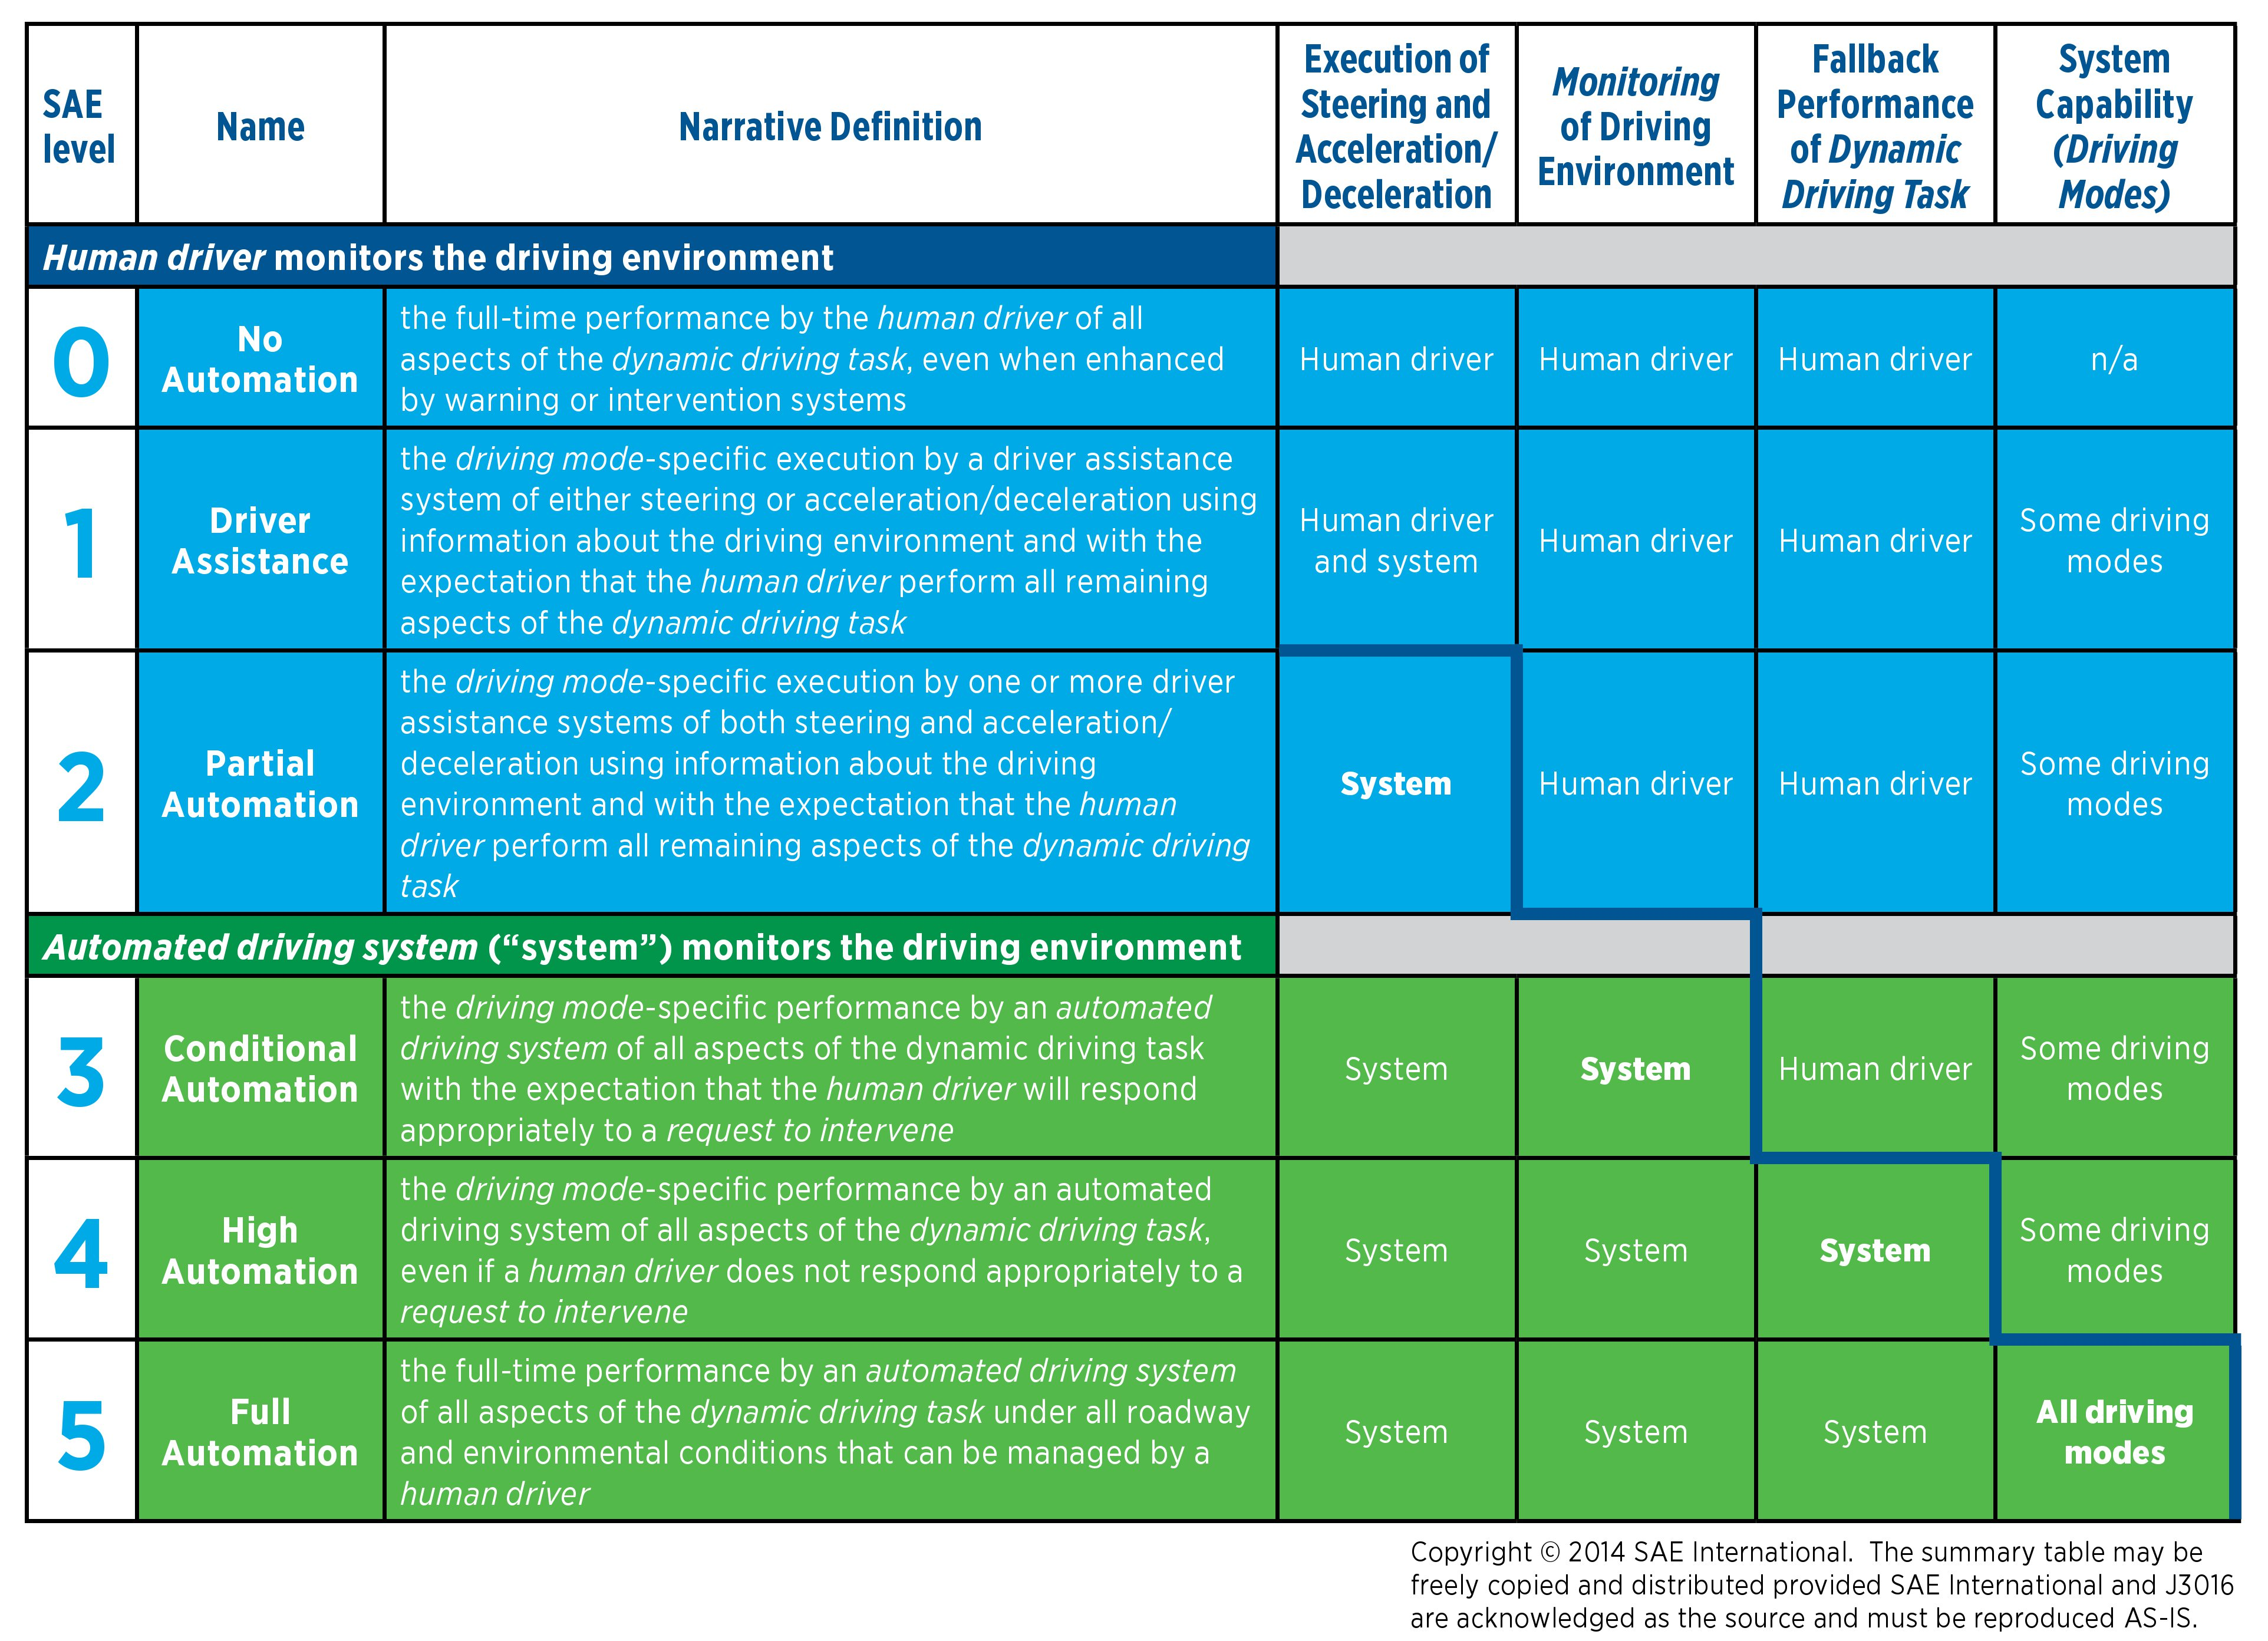
\includegraphics[scale=0.7]{images/level_autonomes_fahren.jpg}
\caption[Norm SAE J3016 für die Stufen des autonomen Fahrens]{Norm SAE J3016 für die Stufen des autonomen Fahrens, entnommen aus \cite{sae2014taxonomy}}
\label{fig_level_autonomes_fahren}
\end{figure}


% ===========================
\subsection{Entwicklung von Fahrerassistenzsystemen}
\label{grundlagen_fahren_entwicklung}
% ===========================

\ac{FAS} sind Funktionen im Kraftfahrzeug, die den Fahrer unterstützen. Diese Systeme nutzen Sensordaten, wie Radar-, Ultraschall-, oder Kameradaten, aus dem Fahrzeug, um den Fahrer dann auf Basis der abgeleiteten Informationen zu unterstützen. Beispielsweise erkennt ein Spurhalteassistent wenn das Fahrzeug die Spur verlässt und kann die Fahrlinie korrigieren. 

Um \ac{FAS} effizient zu entwickeln und schon früh einzelne Komponenten testen zu können, werden diese in der Automobilindustrie häufig mit dem V-Modell als Vorgehensmodell entwickelt. Damit soll die Planungssicherheit und die Qualität der Entwicklung erhöht werden. Das V-Modell ist ein chronologisches Vorgehensmodell und aus der Softwareentwicklung adaptiert \cite{vmodell2005}. Das V-Modell kann in einen linken absteigenden und einen rechten aufsteigenden Ast unterteilt werden. Der linke Ast enthält die Funktionsanforderungen, die nach unten weiter detailliert und aufgeschlüsselt werden. Der rechte Ast umfasst aufsteigend Funktionstests auf dem jeweiligen Detaillierungsgrad \cite{hakuli2015virtuelle}. Das V-Modell ist schematisch in Abbildung \ref{fig_v_modell} dargestellt.

\begin{figure}[h]
\centering
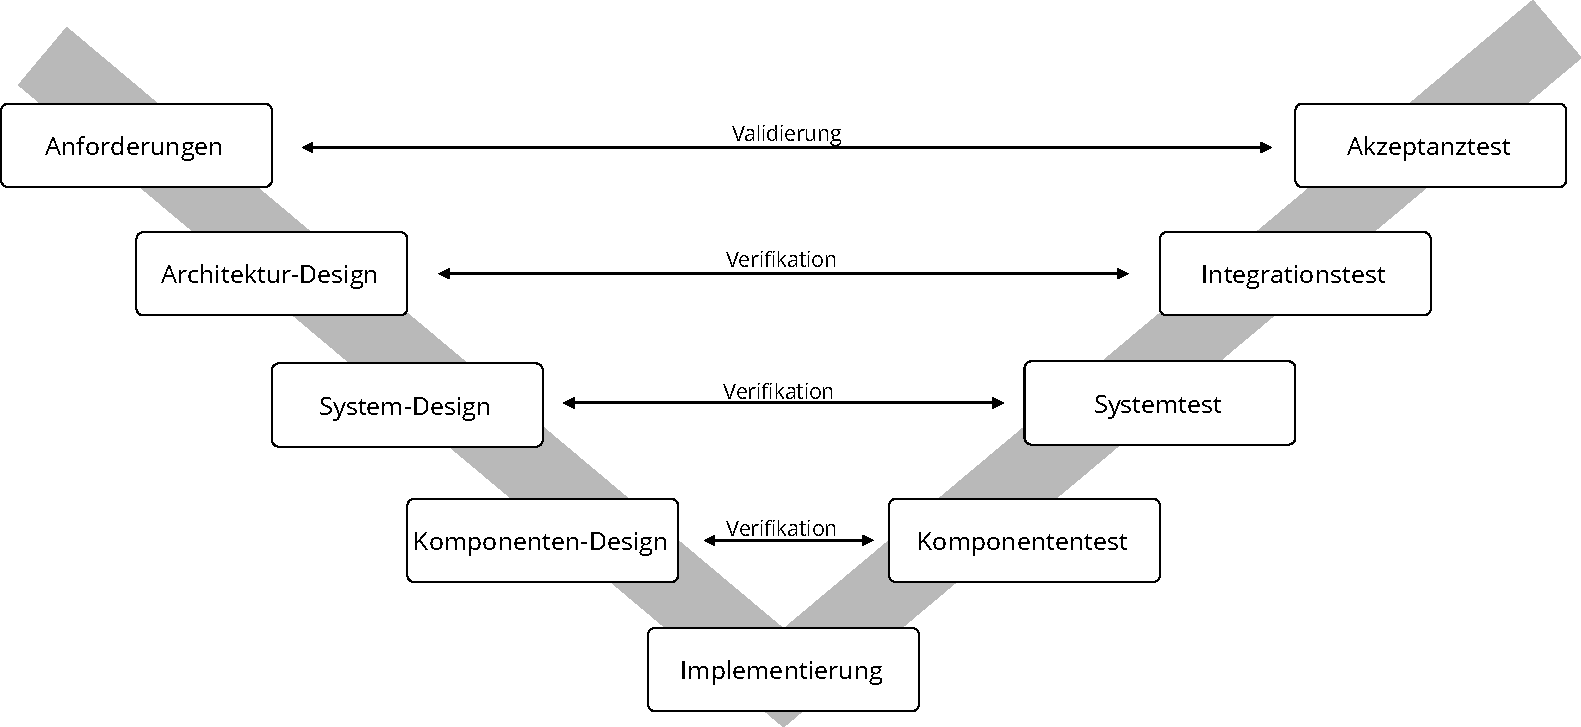
\includegraphics[scale=0.5]{images/v_modell.pdf}
\caption[V-Modell]{V-Modell \cite{hakuli2015virtuelle}}
\label{fig_v_modell}
\end{figure}

Die Schritte auf dem absteigenden und aufsteigenden Ast haben jeweils eine Beziehung. Jeder Test auf dem aufsteigenden Ast verifiziert bzw. validiert den dazugehörigen Entwicklungsschritt auf dem absteigenden Ast. Dementsprechend werden oben im V-Modell die Kundenanforderungen auf dem absteigenden Ast erfasst und auf dem aufsteigenden Ast validiert. Unten im V-Modell werden einzelne Hardware- oder Softwarekomponenten entwickelt, die die entsprechenden Kundenanforderungen von oben lösen sollen. Diese werden anschließend auf dem aufsteigenden Ast verifiziert \cite{hakuli2015virtuelle}.

% ===========================
\subsubsection{Testfälle für die Validierung und Verifikation}
% ===========================

Die Validierung und Verifikation von \ac{FAS} folgt dem Testkonzept. Ein Testkonzept umfasst die Analyse des Testobjektes, die Generierung von Testfällen, die Durchführung von Tests und schließlich die Testauswertung \cite{schuldt2013effiziente}. Diese Schritte sind in der Abbildung \ref{fig_testfallerstellung} dargestellt.

\begin{figure}[h]
\centering
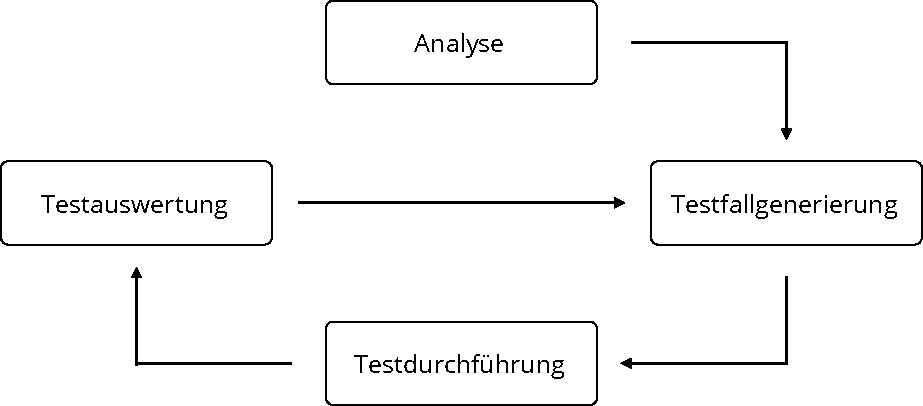
\includegraphics[scale=0.7]{images/testfallerstellung.pdf}
\caption[Schritte zur Testfallerstellung]{Schritte zur Testfallerstellung \cite{schuldt2013effiziente}}
\label{fig_testfallerstellung}
\end{figure}

Testfälle werden bereits möglichst früh im Entwicklungsprozess erstellt, um eine hohe Qualität von \ac{FAS} und einzelnen Komponenten zu erreichen \cite{wachenfeld2015freigabe}. Hierfür werden in der Praxis virtuelle Fahrversuche eingesetzt. Die Idee ist eine stufenweise Digitalisierung von Komponenten aus dem realen Fahrversuch mit den Zielen die Reproduzierbarkeit zu steigern, den Aufwand zu reduzieren und insgesamt flexibler zu werden. Im virtuellen Fahrversuch werden in der frühen Konzeptphase alle Komponenten virtuell getestet und dann schrittweise durch Hardwarekomponenten ersetzt. Schließlich werden alle Komponenten im realen Fahrversuch auf der Straße mit einem realem Fahrer und anderen Verkehrsteilnehmern getestet \cite{hakuli2015virtuelle}.

Beim virtuellen Fahrversuch spielen die Konzepte \ac{MiL}, \ac{SiL}, \ac{HiL} und \ac{ViL} eine wichtige Rolle. Mit \ac{MiL} und \ac{SiL} werden Funktionen auf Basis von Simulationsmodellen getestet \cite{berg2015vehicle}, indem Hardwarekomponenten simuliert werden. Mit fortschreitender Entwicklung werden immer mehr Simulationskomponenten durch die entsprechende Hardware ersetzt und mit \ac{HiL} getestet \cite{hakuli2015virtuelle}. \ac{ViL} schließt schließlich die Lücke zwischen virtuellem Fahrversuch und realem Fahrversuch. Für die Freigabe von \ac{FAS} ist die Realfahrt die wichtigste Methode, da sie aktuell die beste Validierung bei annehmbaren ökonomischen Aufwand ist \cite{wachenfeld2015freigabe}.

Mit steigender Automatisierung von \ac{FAS} steigt die Anzahl möglicher Szenarien, in denen die Sicherheit der Funktionen auch ohne Fahrer garantiert sein muss. Um alle Funktionen ausreichend testen zu können, steigt die Anzahl der benötigten Testfälle. Testfälle müssen alle potentiell eintretenden Szenarien, in denen das \ac{FAS} zum Einsatz kommen kann, abdecken. Dadurch steigt mit hochautomatisierten Funktionen der Aufwand für die Validierung und Verifikation \cite{bach2017reactive}. Eine Möglichkeit für die Reduzierung von Testfällen ist es, kritische Situationen zu finden und Testfälle mit weniger kritischen Situationen zu entfernen \cite{wachenfeld2015freigabe}.

Heute werden Testfälle auf der Basis von Anforderungen an die Fahrfunktionen und Standardsituationen abgeleitet und getestet. Dabei wächst heute schon, mit der Beschränkung auf Standardfälle, der Testaufwand \cite{surmund2018neue}. Mit zukünftigen hochautomatisierten \ac{FAS} ab Stufe 3 des autonomen Fahrens muss das System in allen potentiellen Szenarien sicher sein und Testfälle dürfen nicht mehr auf die Standardsituationen begrenzt sein. Die Sicherheit des Gesamtsystems muss in breiterem Spektrum mit einer Vielzahl Szenarien ohne Eingriff des Fahrers garantiert werden können. Das bedeutet, dass die bisherigen Standardsituationen um neue Szenarien erweitert werden müssen \cite{surmund2018neue}.

Für die Erstellung von Testfällen müssen daher alle potentiell eintretenden kritischen Szenarien bekannt sein. Das Ziel dieser Arbeit ist es, bekannte Szenarien zu klassifizieren und auf diese Weise bisher unbekannte und möglicherweise kritische Szenarien zu finden. Dies soll mit Hilfe von simulierten Daten geschehen, um die Skalierbarkeit mit angemessenem Aufwand garantieren zu können. Das Konzept hierzu wird im Detail in Kapitel \ref{konzept} vorgestellt.

 Im nächsten Abschnitt werden andere Arbeiten, welche die Klassifizierung von Szenarien untersucht haben, vorgestellt und wichtige Grundbegriffe definiert.


% ===========================
\subsection{Klassifizierung von Szenarien}
\label{grundlagen_fahren_szenarien}
% ===========================

In diesem Abschnitt werden zu Beginn die Terminologien von Szene, Situation und Szenario unterschieden und definiert. Im Anschluss wird auf bisherige Arbeiten zur Szenarienerkennung eingegangen.

In dieser Arbeit werden Szene, Situation und Szenario nach Ulbrich et al. \cite{ulbrich2015defining} definiert. In Abbildung \ref{fig_relation_sc_sc} wird die Beziehung zwischen Szene und Szenario dargestellt.

\vspace{0,3cm}
\noindent\textbf{Szene}\\
Eine Szene ist eine Momentaufnahme von der Umgebung einschließlich der räumlichen Szenerie,  allen dynamischen Elementen, der Selbstdarstellung aller Akteure und Beobachter, sowie die Beziehung zwischen diesen Entitäten. Nur in einer Simulation kann eine Szene vollständig und allumfassend beobachtet und erfasst werden (Ground Truth). In der realen Welt dagegen ist die Beschreibung einer Szene immer unvollständig, fehlerhaft, unsicher und subjektiv von einem oder mehreren Beobachtern.

\vspace{0,3cm}
\noindent\textbf{Situation}\\
Eine Situation ist die Gesamtheit aller Umstände, die für die Auswahl einer angemessenen Entscheidung zu einem bestimmten Zeitpunkt berücksichtigt werden müssen. Sie umfasst alle relevanten Zustände, Möglichkeiten und Einflussgrößen für ein Verhalten. Eine Situation wird abgeleitet von einer Szene durch die Auswahl von Informationen basierend auf kurzzeitigen sowie langfristigen Zielen und Werten. Eine Situation ist daher per Definition immer subjektiv von einem Beobachter.

\vspace{0,3cm}
\noindent\textbf{Szenario}\\
Ein Szenario besteht aus mehreren aufeinander folgenden Szenen und beschreibt deren zeitliche Entwicklung. Handlungen, Ereignisse, Ziele und Werte können für eine Charakterisierung der zeitlichen Entwicklung eines Szenarios spezifiziert werden. im Gegensatz zu einer Szene, umfasst ein Szenario einen definierten Zeitraum.

\vspace{0,3cm}

\begin{figure}[h]
\centering
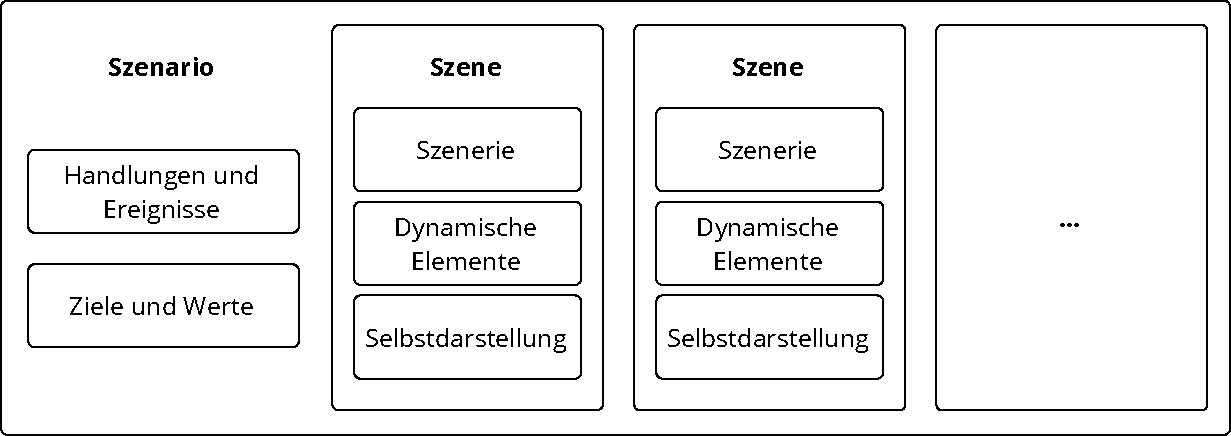
\includegraphics[scale=0.7]{images/relation_sc_sc.pdf}
\caption[Zusammenhang zwischen Szene und Szenario]{Zusammenhang zwischen Szene und Szenario \cite{ulbrich2015defining}}
\label{fig_relation_sc_sc}
\end{figure}

Neben den Begriffen Szene, Situation und Szenario wird oft der Begriff Manöver verwendet. Bach et al. \cite{bach2016model} definieren ein Manöver als einen Zustand innerhalb eines Szenarios. Dabei sind Situationen jeweils Übergangsbedingungen zwischen einzelnen Manövern. So setzt sich beispielsweise das Szenario \textit{Überholen} aus den Manövern \textit{Spurwechsel nach links}, \textit{Beschleunigung}, \textit{Spurwechsel nach rechts} und \textit{Bremsvorgang} zusammen. Zwischen den einzelnen Manövern gibt es Situation wie \textit{langsameres Auto voraus} oder \textit{langsameres Auto links überholt}, die jeweils ein neues Manöver einleiten.

Je nachdem, wie granular Szenarien bzw. wie grob Manöver definiert werden, können Szenarien und Manöver nicht klar voneinander abgegrenzt werden. So kann ein einzelnes Manöver auch bereits ein gesamtes Szenario darstellen. Zum Beispiel kann das Manöver \textit{Spurwechsel} bereits als Szenario definiert werden. Aus diesem Grund wird in dieser Arbeit im Folgenden ausschließlich von Szenarien gesprochen.

Da sich diese Arbeit größtenteils auf die Klassifizierung von Szenarien fokussiert, wird in den folgenden Absätzen eine erweiterte Definition von Szenarien nach Bagschik et al. \cite{bagschik2017szenarien} gegeben. Diese Definition unterteilt den Begriff in drei weitere Abstraktionsebenen: Funktionale, logische und konkrete Szenarien.

Funktionale Szenarien sind auf der semantischen Ebene formuliert. Entitäten und Beziehungen werden widerspruchsfrei in sprachlichen Texten beschrieben. Dabei ist das Vokabular klar definiert und wird eindeutig für alle zu beschreibenden Szenarien verwendet. Je nachdem wie detailliert ein Szenario beschrieben werden soll, muss ein geeignetes Vokabular definiert werden. Funktionale Szenarien können in einzelne oder mehrere logische Szenarien überführt werden.

Logische Szenarien sind detaillierter als funktionale Szenarien, indem  Entitäten und Beziehung in quantitive Parameterbereiche übersetzt werden. Parameterbereiche können dabei mit statistischen Verteilungen (Normalverteilung, Gleichverteilung etc.) modelliert werden. Zusätzlich können Beziehungen zwischen Entitäten mit numerischen Bedingungen (e.g. Fahrzeug A muss auf derselben Spur fahren wie Fahrzeug B) oder Korrelationsfunktionen (e.g. Abstand zwischen Fahrzeug A und Fahrzeug B in Abhängigkeit der Geschwindigkeit) ausgedrückt werden.

Konkrete Szenarien haben den höchsten Detailgrad und Entitäten und Beziehungen werden mit festen Parametern definiert. Logische Szenarien können in einzelne oder mehrere konkrete Szenarien überführt werden.

Ein Beispiel zu jeder Abstraktionsebene (funktional, logisch, konkret) ist in Abbildung \ref{fig_funktional_logisch_konrekt} gegeben.

\begin{figure}[h]
\centering
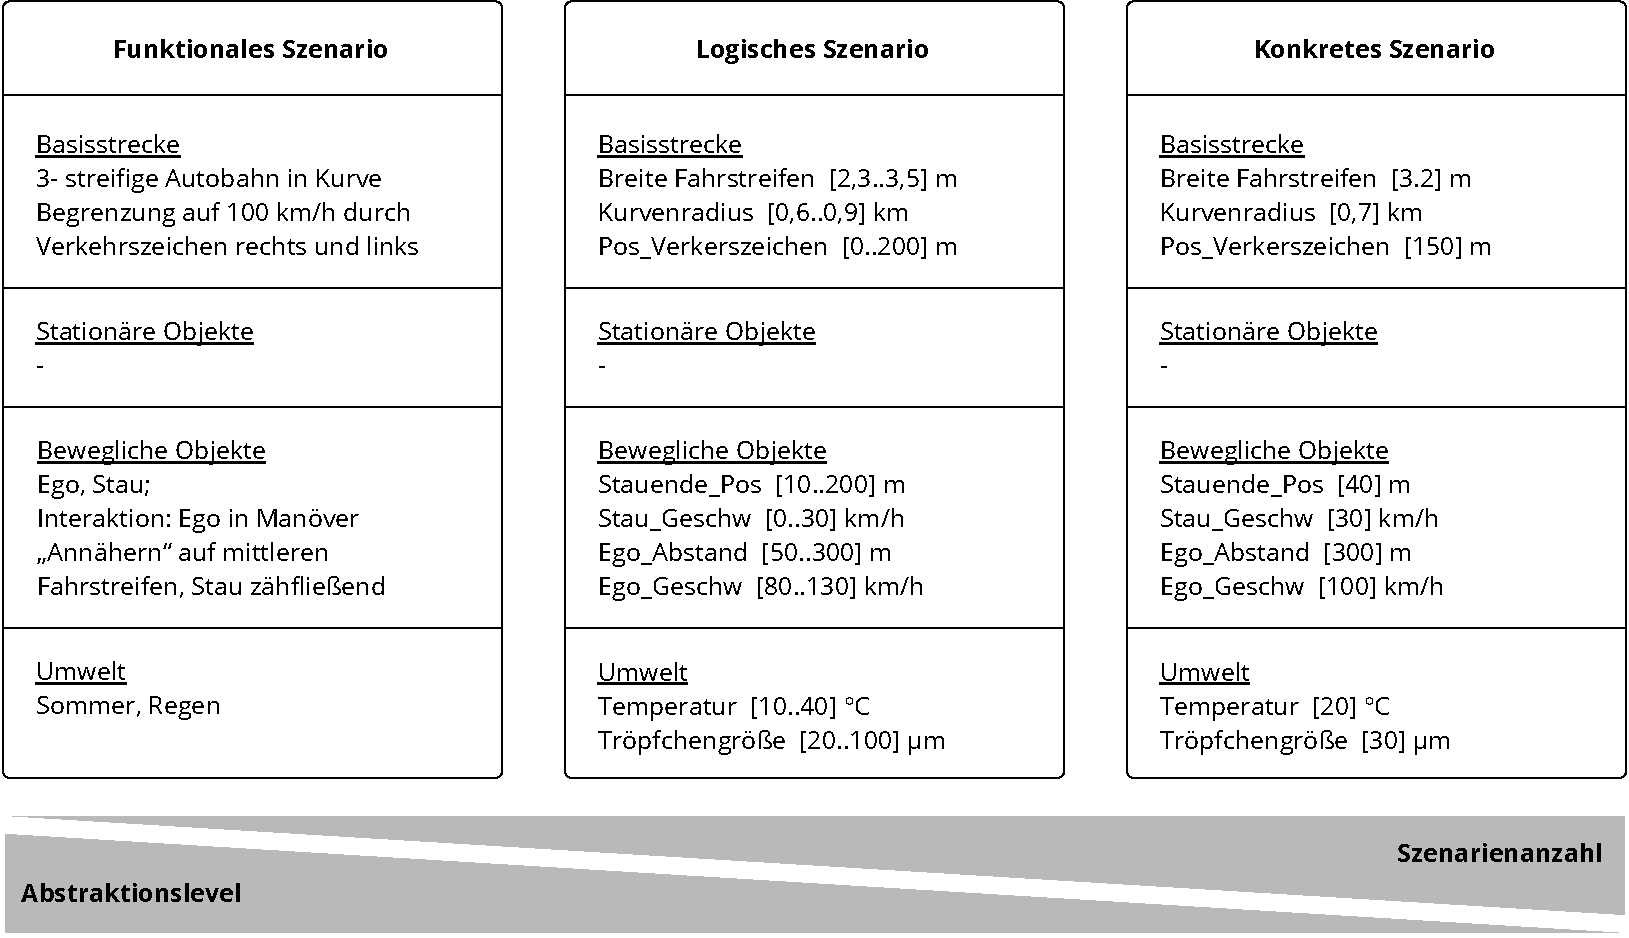
\includegraphics[scale=0.5]{images/funktional_logisch_konrekt.pdf}
\caption[Beispiel für ein funktionales, logisches und konkretes Szenario]{Beispiel für ein funktionales, logisches und konkretes Szenario \cite{bagschik2017szenarien}}
\label{fig_funktional_logisch_konrekt}
\end{figure}


% ===========================
\subsubsection{Bisherige Arbeiten zur Klassifizierung von Fahrszenarien}
% ===========================

Wie in Abschnitt \ref{grundlagen_fahren_entwicklung} beschrieben ist die Klassifizierung von Szenarien ein wichtiges Element für die Erstellung von Testfällen und die Sicherung von \ac{FAS}. In den vergangenen Jahren wurden bereits einige Arbeiten zur Klassifizierung von Szenarien veröffentlicht. In den folgenden Absätzen werden jeweils die Datenbasis, die Klassifizierungsmethode und die jeweiligen Fahrszenarien der bisherigen Arbeiten seit 2014 kurz vorgestellt.

Für die Klassifizierung wurden verschiedene Sensordaten aus dem Fahrzeug verwendet. Die Autoren von fünf Arbeiten haben Beschleunigungs-, Gyroskop-, GPS- und Magnetometer-Daten mithilfe eines Smartphones in einem Fahrzeug aufgezeichnet \cite{xie2018driving, cervantes2016vehicle, woo2016manoeuvre, camlica2016feature, arroyo2016adaptive}. Die Verwendung von Smartphone-Daten wurde mit der einfachen und kostengünstigen Umsetzung begründet. Vier andere Arbeiten verwendeten Sensordaten wie \textit{Lenkwinkel}, \textit{Fahrzeuggeschwindigkeit}, \textit{laterale Geschwindigkeit}, \textit{Giergeschwindigkeit} und die \textit{Position des Gas- und Bremspedals}, die sie aus dem CAN-Bus des Fahrzeugs auslasen \cite{zheng2017lane, zheng2015non, li2015lane, zheng2014threshold}. Drei weitere Arbeiten basierten ihre Experimente auf Daten aus einem Fahrsimulator \cite{sun2017robust, zheng2016drivers} und realen Testfahrten \cite{gruner2017spatiotemporal}. Die verwendeten Daten waren der \textit{laterale Abstand zwischen Fahrzeug und Fahrbahnmarkierung}, \textit{Spurabfahrtsbetrag}, \textit{Beschleunigung}, \textit{Lenkwinkel}, \textit{Lenkgeschwindigkeit}, \textit{Lenkmoment} und \textit{Ort}, \textit{Ausrichtung}, und \textit{Geschwindigkeit} des Ego-Fahrzeugs und benachbarten Objekten. Dabei wurde nicht weiter spezifiziert, wie die Daten ausgelesen wurden.

Auf Basis der Sensordaten wurden verschiedene Klassifikatoren erstellt. Es wurden die Methoden \ac{SVM} \cite{sun2017robust, cervantes2016vehicle, woo2016manoeuvre, camlica2016feature, zheng2016drivers, zheng2015non}, \ac{RF} \cite{xie2018driving, cervantes2016vehicle, zheng2016drivers}, \ac{kNN} \cite{zheng2017lane, camlica2016feature, zheng2016drivers}, \ac{HMM} \cite{zheng2017lane, li2015lane}, \ac{FRC} \cite{cervantes2016vehicle, arroyo2016adaptive}, Bayesian Inference Model \cite{sun2017robust}, \ac{CNN} \cite{gruner2017spatiotemporal}, Decision Tree \cite{zheng2014threshold} und Naive Bayes \cite{camlica2016feature} verwendet. Da die Methoden für diese Arbeit nicht weiter relevant sind, werden sie an dieser Stelle nicht im Detail erläutert, es wird lediglich auf die jeweiligen Quellen verwiesen.

In Tabelle \ref{tab_szenarienerkennung} sind alle dem Autor bekannten Arbeiten seit 2014 zusammengefasst. Neben den verwendeten Methoden zur Klassifizierung sind die jeweils verwendeten Sensordaten und die klassifizierten Szenarien aufgeführt.

\begin{longtable}[c]{p{1,5cm} p{4.5cm} p{2,5cm} p{4.5cm}}
\textbf{Quelle} & \textbf{Sensordaten} & \textbf{Klassifikator} & \textbf{Szenarien} \\
\hline
\endhead

\cite{xie2018driving} & Beschleunigung, Gyroskop und GPS von einem Smartphone im Fahrzeug & \ac{RF} & Abbiegen, links abbiegen, rechts abbiegen, beschleunigen, bremsen, stoppen, Spurwechsel nach links, Spurwechsel nach rechts \\
\hline

\cite{zheng2017lane} & Lenkwinkel und Fahrzeuggeschwindwigkeit aus dem CAN-Bus & \ac{kNN}, \ac{HMM} & Spurwechsel nach links, Spurwechsel nach rechts, Spur halten \\
\hline

\cite{sun2017robust} & Lateraler Abstand zwischen Fahrzeug und Fahrbahnmarkierung von einem Fahrsimulator & \ac{SVM}, Bayesian Inference Model & Spurwechsel nach links, Spurwechsel nach rechts, Spur halten \\
\hline

\cite{gruner2017spatiotemporal} & Ort, Ausrichtung und Geschwindigkeit des Ego-Fahrzeugs und benachbarten Objekten von realen Testfahrten & \ac{CNN} auf Basis von gestapelten Positionsgittern der Objekte & Frei fahren, anderes Fahrzeug voraus, anderes Fahrzeug überholt Ego-Fahrzeug, Querverkehr vor Ego-Fahrzeug \\
\hline

\cite{cervantes2016vehicle} & Beschleunigung von einem Smartphone im Fahrzeug & \ac{RF}, \ac{SVM}, \ac{FRC} & Einparken, geparkt, frei fahren, stoppen \\
\hline

\cite{woo2016manoeuvre} & Beschleunigung, Gyroskop, GPS und Magnetometer von einem Smartphone im Fahrzeug & \ac{SVM} & Stoppen, beschleunigen, bremsen, links abbiegen, rechts abbiegen \\
\hline

\cite{camlica2016feature} & Beschleunigung, Gyroskop und GPS von einem Smartphone im Fahrzeug & \ac{SVM}, \ac{kNN}, Naive-Bayes & Stoppen, beschleunigen, frei fahren, bremsen, Spurwechsel nach links, Spurwechsel nach rechts, links abbiegen, rechts abbiegen, in Kreisverkehr eintreten, aus Kreisverkehr austreten \\
\hline

\cite{zheng2016drivers} & Spurabfahrtsbetrag, Beschleunigung, Lenkwinkel, Lenkgeschwindigkeit und Lenkmoment von einem Fahrsimulator & \ac{SVM}, \ac{kNN}, \ac{RF} & Spurwechsel nach links, Spurwechsel nach rechts, Spur halten \\
\hline

\cite{arroyo2016adaptive} & Beschleunigung, Gyroskop und GPS von einem Smartphone im Fahrzeug & \ac{FRC} & Lenken, beschleunigen, bremsen, Bodenwelle \\
\hline

\cite{zheng2015non} & Fahrzeuggeschwindigkeit und Lenkwinkel aus dem CAN-Bus & \ac{SVM} & links abbiegen, rechts abbiegen, Spurwechsel nach links, Spurwechsel nach rechts, Kurve nach links, Kurve nach rechts, geradeaus fahren, stoppen \\
\hline

\cite{li2015lane} & Fahrzeuggeschwindigkeit, Position des Gas- und Bremspedals, Lenkwinkel, Laterale Beschleunigung und Giergeschwindigkeit aus dem CAN-Bus & \ac{HMM} & Spurwechsel nach links, Spurwechsel nach rechts, Spur halten \\
\hline

\cite{zheng2014threshold} & Fahrzeuggeschwindigkeit, Lenkwinkel, Drehzahl und Position des Gas- und Bremspedals aus dem CAN-Bus & Decision Tree auf Basis von Schwellenwerten & links abbiegen, rechts abbiegen, Spurwechsel nach links, Spurwechsel nach rechts, Kurve nach links, Kurve nach rechts, geradeaus fahren, stoppen \\

\hline
\caption{Bisherige Arbeiten zur Szenarienerkennung}
\label{tab_szenarienerkennung}
\end{longtable}

Die Datenerhebungen in den vergangenen Arbeiten wurden vor dem Hintergrund durchgeführt, vordefinierte Szenarien zu erkennen. Von diesen Szenarien wurden die benötigten Sensordaten abgeleitet und dann mit bestimmten Methoden verschiedene Klassifikatoren erstellt. Bis auf in der Arbeit von Gruner \cite{gruner2017spatiotemporal} werden für die Klassifizierung von Fahrszenarien bisher keine \acp{DNN} verwendet. Ebenfalls verwendet Gruner in seiner Arbeit keine Kamerabilder, sondern gestapelte Matrizen, auf denen jeweils die Positionen aller Verkehrsteilnehmer markiert sind. Nach Gruner \cite{gruner2017spatiotemporal} wird sich die zukünftige Forschung mit tieferen Netzstrukturen wie \acp{RNN} beschäftigen, um zeitabhängige Szenarien noch besser zu verstehen.

Mit den bisherigen Ansätzen können bekannte Szenarien sehr zuverlässig erkannt werden. Bisher unbekannte Szenarien werden allerdings nur sehr bedingt erkannt, weil die Datengrundlage auf Basis der bekannten Szenarien optimiert ist. Das bedeutet, dass Daten, die für die Erkennung von bisher unbekannten Szenarien möglicherweise relevant sind, nicht erfasst und daher nicht für die Erstellung des Klassifikators verwendet werden.

Im Gegensatz zu den bisherigen Arbeiten, soll in dieser Arbeit die Verwendung von Kameradaten für die Klassifizierung von Szenarien untersucht werden. Die Idee ist, dass Videodaten den gleichen Informationsgehalt besitzen wie das Sichtfeld eines realen Fahrers. Ein Fahrer kann auf Basis seines Sichtfeldes alle Szenarien erkennen und auf der Basis die Umgebung und alle Fahrfunktionen überwachen. Da in Zukunft das System diese Aufgabe übernehmen wird, soll in dieser Arbeit ein Klassifikator mit genau diesem Sichtfeld, mit Videodaten, trainiert werden. Damit sollen auch bisher unbekannte Einflüsse, die auf den Bildern zu sehen sind, für die Klassifizierung berücksichtigt werden. In einem weiteren Schritt kann ein Klassifikator, der auf diese Weise mit allen bisher bekannten Szenarien trainiert wurde, bekannte Szenarien erkennen und bisher unbekannte Szenarien identifizieren. Der Ansatz wird im Detail in Kapitel \ref{konzept} vorgestellt.

% ===========================
\section{Künstliche Neuronale Netze}
\label{grundlagen_nn}
% ===========================

In diesem Kapitel werden künstliche Neuronale Netze (\acp{KNN}) mit einem Schwerpunkt auf Bilderkennung mit Convolutional Neural Networks (\acp{CNN}) und Sequenzerkennung mit \acfp{LSTM} eingeführt. Im folgenden Abschnitt \ref{grundlagen_nn_ml} werden \acp{KNN} in den Gesamtkontext von maschinellem Lernen gestellt. Im Anschluss werden in Abschnitt \ref{grundlagen_nn_entwicklung} die Grundlagen zu \acp{KNN} erläutert. Danach werden komplexe Architekturen von \acp{KNN} zur Bilderkennung in Abschnitt \ref{grundlagen_nn_cnn} und zur Sequenzerkennung in Abschnitt \ref{grundlagen_nn_rnn} erklärt. In Abschnitt \ref{grundlagen_nn_synthetisch} wird auf das Training mit synthetischen Daten eingegangen und im letzten Abschnitt \ref{grundlagen_nn_video} wird die aktuelle Forschung zu Videoklassifizierung vorgestellt.

% ===========================
\subsection{Einordnung im maschinellen Lernen}
\label{grundlagen_nn_ml}
% ===========================

Maschinelles Lernen wird oft als ein Teil des Bereichs künstliche Intelligenz beschrieben. Dabei wird maschinelles Lernen nach Mitchell \cite{mitchell1997machine} wie folgt definiert:

\begin{quote}
\textit{\glqq Ein Computerprogramm lernt aus der Erfahrung E in Bezug auf eine Klasse von Aufgaben T und dem Leistungsmaß P, wenn seine Leistung, gemessen mit P, bei Aufgaben aus T sich mit Erfahrung E verbessert.\grqq}
\end{quote}

Da maschinelles Lernen sehr viele Bereiche umfasst, wird hier nur auf die relevanten Teile für diese Arbeit eingegangen und auf \cite{mitchell1997machine} verwiesen. Maschinelles Lernen kann in drei verschiedenen Kategorien eingeteilt werden. Diese werden in den folgenden Absätzen beschrieben.

Überwachtes Lernen (engl. supervised learning) beschreibt einen Lernprozess, in dem die Trainingsdaten sowohl Inputvektoren als auch die zugehörigen Zielvektoren enthalten \cite{bishop2006pattern}. Ein Beispiel dafür ist ein Klassifizierungsproblem von Buchstaben, bei dem sowohl die Bilder der einzelnen Buchstaben, als auch deren zugehörige Klasse (abgebildeter Buchstabe) einem Trainingsalgorithmus übergeben werden. Neben Klassifizierungsproblemen fallen auch Regressionsprobleme in diese Kategorie.

Beim unüberwachten Lernen (engl. unsupervised learning) enthalten die Trainingsdaten ausschließlich die Inputvektoren, ohne die dazugehörigen Zielvektoren. Das Ziel dabei ist es, Muster in den gegebenen Daten zu erkennen, um beispielsweise Cluster zu bilden \cite{bishop2006pattern}. Das Clustering von Kundengruppen, die bisher unbekannt waren, fällt in diese Kategorie des maschinellen Lernens.

Das verstärkende Lernen (engl. reinforcement learning) ist eine Methodik in welcher der Trainingsalgorithmus mit Situationen konfrontiert wird und jeweils aus einer Reihe von gegebenen Handlungen wählen kann. Das Ziel dabei ist es, das Endergebnis, das auf der Wahl aller Handlungen basiert, zu maximieren \cite{sutton1998introduction}. Ein Beispiel hierfür ist das selbstständige Erlernen des Brettspiels Schach.


% ===========================
\subsubsection{Klassifizierung}
% ===========================

In dieser Arbeit wird ein Konzept für die Klassifizierung von Fahrszenarien - damit in der Kategorie des überwachten Lernens - entwickelt und umgesetzt. Das Ziel von Klassifizierungsalgorithmen ist es, gegebene Objekte auf Basis ihrer Eigenschaften einer Klasse zuzuordnen. Dabei sollen die Objekte innerhalb einer Klasse eine möglichst geringe Varianz und zwischen verschiedenen Klassen eine möglichst hohe Varianz besitzen. Klassifizierungsalgorithmen arbeiten dafür mit Trainingsdaten, die aus Inputvektoren und Zielvektoren bestehen. Ein Inputvektor enthält alle Eigenschaften und der Zielvektor die jeweilige Klasse des Objekts. In Abbildung \ref{fig_klassifizierung} ist beispielhaft die Klassifizierung eines Datensatzes mit zwei Klassen dargestellt. Die Objekte im Datensatz haben jeweils die Eigenschaften $x_1$ und $x_2$.

\begin{figure}[h]
\centering
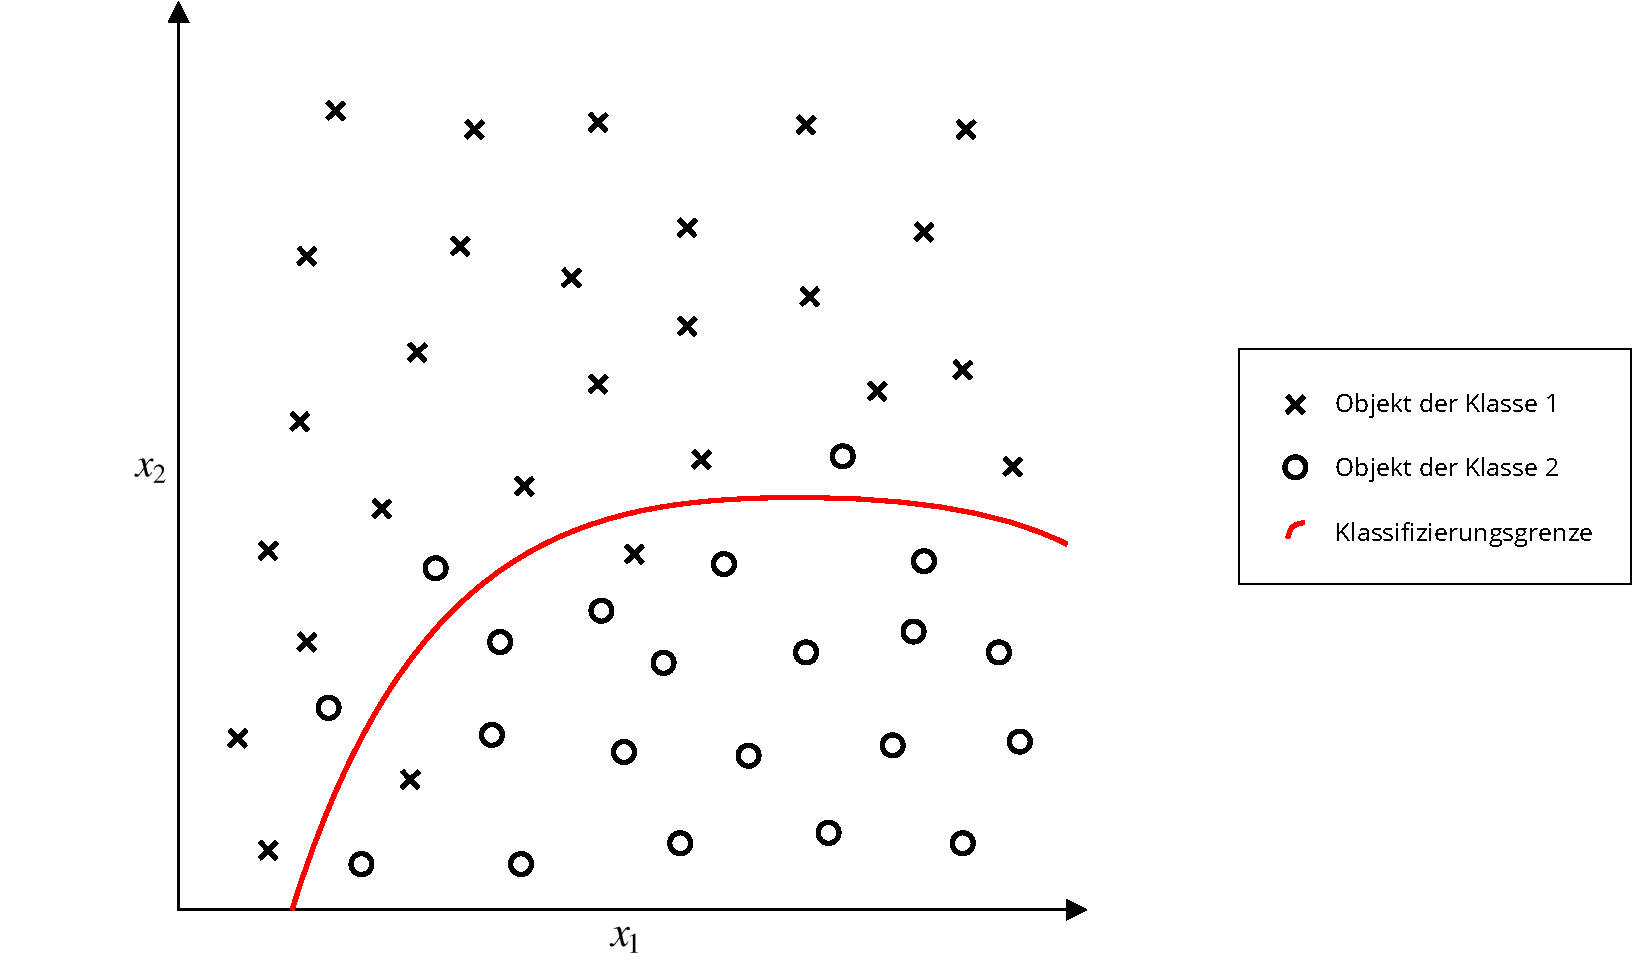
\includegraphics[scale=0.5]{images/klassifizierung.pdf}
\caption{Beispiel einer Klassifizierung mit zwei Klassen}
\label{fig_klassifizierung}
\end{figure}

In den folgenden Abschnitten werden schrittweise \acp{CNN} und \acp{LSTM} eingeführt. Mit diesen Komponenten werden später verschiedene Klassifikatoren für die Erkennung von Fahrszenarien entwickelt und trainiert.


% ===========================
\subsection{Entwicklung von künstlichen neuronalen Netzen}
\label{grundlagen_nn_entwicklung}
% ===========================

\acp{KNN} wurden ursprünglich als ein Modell der Informationsverarbeitung von biologischen Gehirnen entwickelt \cite{mcculloch1943logical}. Dabei ist die kleinste Einheit in einem \ac{KNN} ein einzelnes Neuron. Rosenblatt \cite{rosenblatt1958perceptron} entwickelte ein Modell eines Neurons als binären Klassifikator. Dieses sogenannte Perzeptron setzt sich aus einem Eingangsvektor $x_1, ..., x_n$, einem Vektor mit Gewichten $w_1, ..., w_n$, einer Summenfunktion $\sum$, einer Aktivierungsfunktion $\varphi$ mit einem Schwellenwert $\theta$ und einem Aktivierungswert $o(\vec{x})$ zusammen. Abbildung \ref{fig_perceptron} zeigt das Modell eines Perzeptrons.

\begin{figure}[h]
\centering
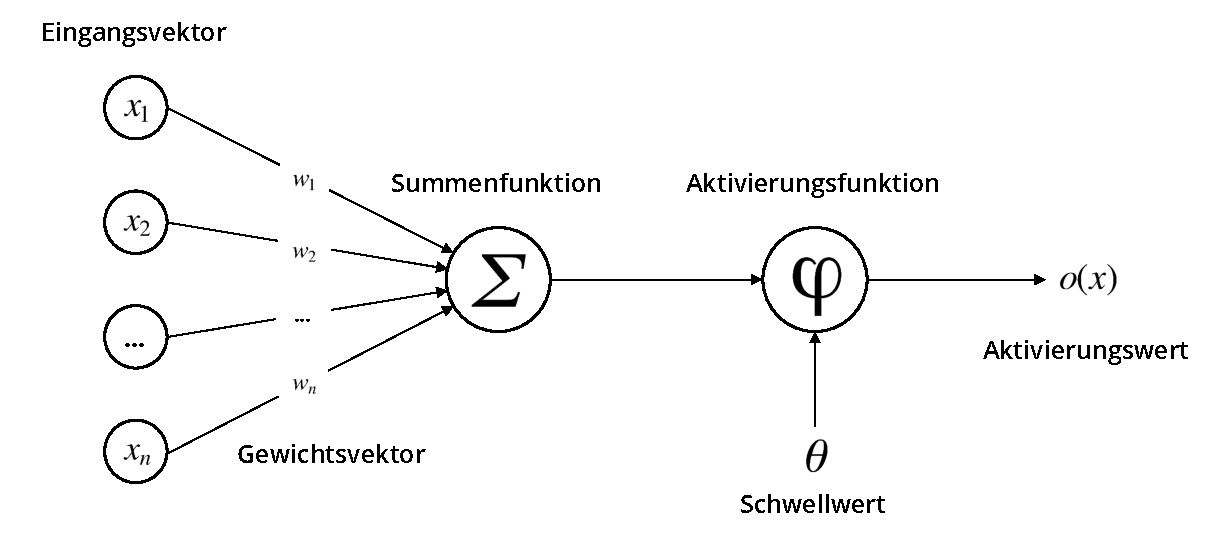
\includegraphics[scale=0.7]{images/perceptron.pdf}
\caption[Modell eines Perzeptrons]{Modell eines Perzeptrons \cite{rosenblatt1958perceptron}}
\label{fig_perceptron}
\end{figure}

Um den Aktivierungswert $o(\vec{x})$ zu berechnen wird zunächst die gewichtete Summe mit dem Eingangsvektor $\vec{x}$ und den Gewichten $\vec{w}$ gebildet. Im Anschluss wird mit der Aktivierungsfunktion $\varphi$ eine Klasse bestimmt. Beim ursprünglichen Perzeptron handelt es sich dabei um eine Schwellenwertfunktion, welche die zwei Werte $-1$ und $1$ annehmen kann. Damit ist das Perzeptron ein binärer Klassifikator und kann die logischen Operationen \textit{AND}, \textit{OR} und \textit{NOT} ausführen. Die logische Operation \textit{XOR} kann mit einem einzelnen Perzeptron nicht abgebildet werden \cite{minski1969perceptrons}.

\begin{equation}
\varphi(\vec{x}, \vec{w}) = \begin{cases} 1 \qquad \text{wenn} \quad \vec{x}*\vec{w} \geq \theta \\ 0 \qquad \text{sonst} \end{cases}
\end{equation}

Die Klassifizierung eines Objekts aus der Klasse $t$ mit den Eigenschaften $\vec{x}$ ist richtig, wenn das Ergebnis $o$ der Aktivierungsfunktion $\varphi(\vec{x},\vec{w})$ der tatsächlichen Klasse des Objekts $t$ entspricht. Wenn die Klasse nicht richtig erkannt wurde $o(\vec{x}) \neq t$, werden die Gewichte $\vec{w}$ entsprechend der Perzeptron-Lernregel angepasst. Diese Lernregel ist ein wichtiger Vorteil von Rosenblatts Perzeptron \cite{rosenblatt1958perceptron} gegenüber des Neurons von McCulloch und Pitts \cite{mcculloch1943logical}, weil die Gewichte erlernt werden können.

Vor dem Training werden die Gewichte $\vec{w}$ zufällig initialisiert. In jedem Trainingsschritt wird überprüft ob die berechnete Klasse $o(\vec{x})$ der tatsächlichen Klasse $t$ entspricht. Wenn $o(\vec{x}) = t$ werden die Gewichte nicht verändert und der nächste Trainingsschritt wird ausgeführt. Wenn $o(\vec{x}) \neq t$ werden die Gewichte nach der Perzeptron-Lernregel aktualisiert:

\begin{equation}
w^{neu}_i = w^{alt}_i + \Delta w_i
\end{equation}
\begin{equation}
\Delta w_i = \eta*(t-o)*x_i
\end{equation}

Die Lernrate $\eta$ kann angepasst werden und bestimmt wie stark die Gewichte in jedem Trainingsschritt verändert werden. Üblicherweise werden Lernraten zwischen $0,01$ und $0,0001$ gewählt.

Neben der Schwellenwertfunktion werden für die Aktivierung von einzelnen Neuronen verschiedene Aktivierungsfunktionen verwendet. Die am meisten verwendeten Funktionen hierfür sind die \ac{tanh}-Funktion

\begin{equation}
\varphi(x) = \tanh(x) = \frac{e^{2x}-1}{e^{2x}+1} \text{,}
\end{equation}

\noindent die Sigmoid- oder S-Funktion

\begin{equation}
\varphi(x) = \frac{1}{1+e^{-x}}
\end{equation}

\noindent und die \ac{ReLU}-Funktion 

\begin{equation}
\varphi(x) = \max{(0, x)}.
\end{equation}

\noindent Diese Funktionen sind, zusammen mit der zuvor vorgestellten Schwellenwertfunktion, in Abbildung \ref{fig_aktivierungsfunktionen} dargestellt.

\begin{figure}[h]
\centering
\begin{tabular}{cc}
\subfloat[Sigmoid]{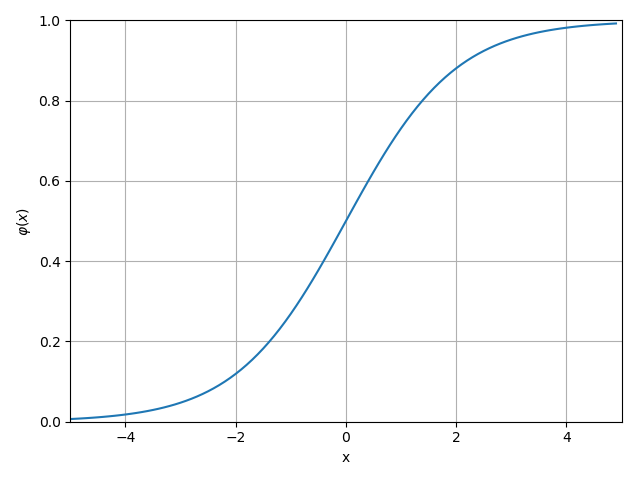
\includegraphics[scale=0.4]{images/act_sigmoid.png}} &
\subfloat[\ac{tanh}]{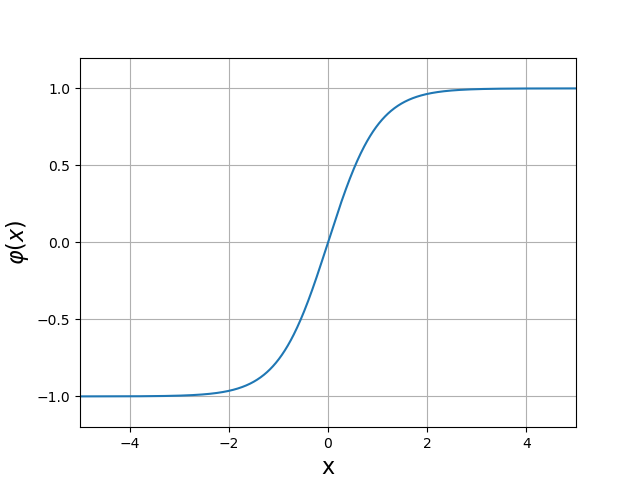
\includegraphics[scale=0.4]{images/act_tanh.png}} \\
\subfloat[\ac{ReLU}]{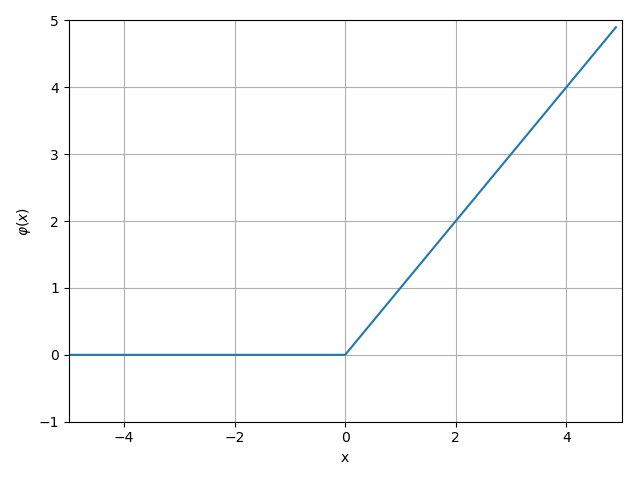
\includegraphics[scale=0.4]{images/act_relu.png}} &
\subfloat[Schwellenwertfunktion]{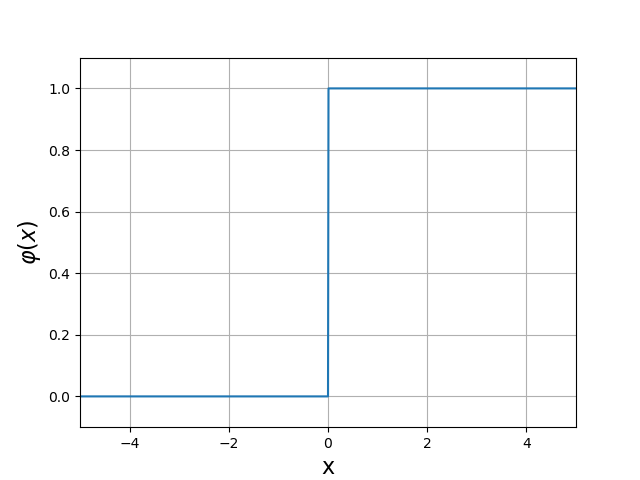
\includegraphics[scale=0.4]{images/act_step_fc.png}}
\end{tabular}
\caption{Aktivierungsfunktionen für Neuronen}
\label{fig_aktivierungsfunktionen}
\end{figure}

Mit diesen Aktivierungsfunktionen und der Verwendung mehrerer Perzeptronen kann ein \acp{KNN}, oder auch mehrlagiges Perzeptron (engl. multilayer perceptron), modelliert werden. Diese Netze können auf unterschiedliche Probleme angewendet werden und überwinden die Schwächen eines einzelnen Perzeptrons (ausschließlich binäre Klassifizierung, keine \textit{XOR}-Operation). Ein mehrschichtiges \ac{KNN} besteht aus mindestens zwei Schichten, einer Ergebnis-Schicht und mindestens einer verborgenen Schicht. Der Eingangsvektor $\vec{x}$ wird nicht als eine Schicht gezählt. Jede Schicht besteht aus $1, ..., n$ Neuronen (Perzeptronen), die im Modell als Knoten modelliert sind. Die Neuronen einer Schicht bestehen jeweils aus einer gewichteten Summe und einer Aktivierungsfunktion und sind jeweils mit dem Eingangsvektor oder den Neuronen der vorherigen und nachfolgenden Schichten verbunden. Diese Verbindungen werden als Kanten modelliert und repräsentieren die Gewichte mit denen die Neuronen verknüpft sind. Abbildung \ref{fig_knn} zeigt das Schema eines dreischichtigen \acp{KNN}.

\begin{figure}[h]
\centering
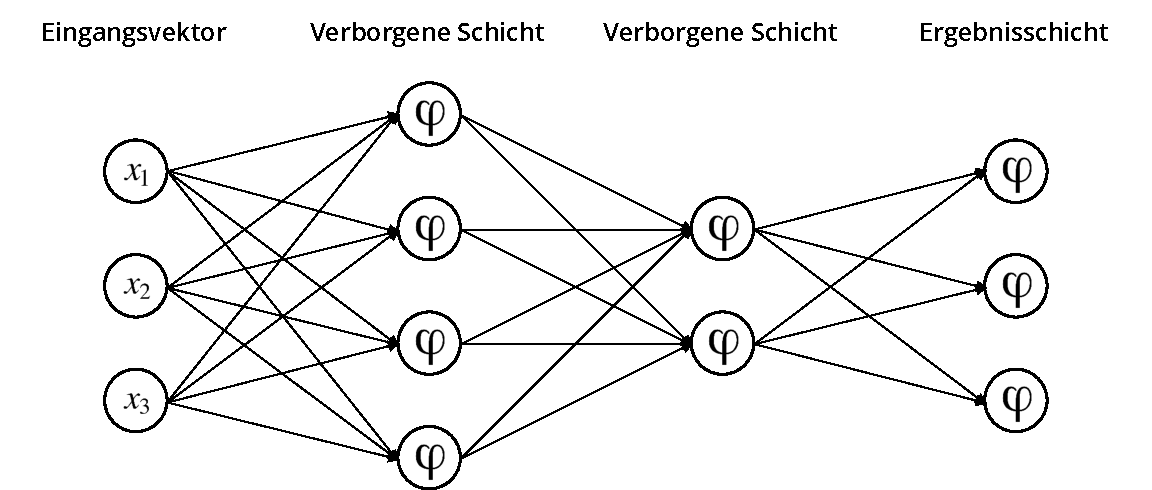
\includegraphics[scale=0.7]{images/knn.pdf}
\caption{Mehrlagiges Perzeptron mit zwei versteckten Schichten}
\label{fig_knn}
\end{figure}

Das Training eines mehrschichtigen \ac{KNN} funktioniert analog zu dem Training eines einzelnen Perzeptrons. In jedem Trainingsschritt wird ein Ergebnis $o(\vec{x})$ berechnet und mit dem richtigen Ergebnis $t$ verglichen. Mit dem Eingangsvektor $\vec{x}$ werden die Aktivierungswerte $y_j$ des Vektors  $\vec{y}$ der ersten verborgenen Schicht wie folgt berechnet:

\begin{equation}
y_j = \varphi(\sum_i{w_{ij}*x_i})
\end{equation}

Dabei ist $w_{ij}$ die Gewichtung der Kante zwischen dem Eingangswert $x_i$ und dem verborgenem Neuron $j$. Alle weiteren verborgenen Schichten sowie der Ergebnisvektor werden auf die gleiche Weise, mit den Aktivierungswerten der vorherigen Schicht als Eingangsvektor, berechnet. Für binäre Klassifizierungsprobleme kann beispielsweise die Sigmoid-Funktion als Aktivierungsfunktion für die Ergebnisschicht gewählt werden. Dann ist das Ergebnis $o$ eine Zahl zwischen $0$ und $1$ und beschreibt die Wahrscheinlichkeit, dass der Eingangsvektor $\vec{x}$ zur Klasse $c_1$ gehört. Dementsprechend beschreibt $1-o$ die Wahrscheinlichkeit der Klasse $c_2$. Bei Klassifizierungsproblemen mit mehreren Klassen wird häufig die Softmax-Funktion als Aktivierungsfunktion $\varphi$ gewählt, um die Wahrscheinlichkeiten der einzelnen Klassen $c_k$ zu bestimmen \cite{bridle1990probabilistic}:

\begin{equation}
o_k = p(c_k|x) = \frac{e^{x^\top w}}{\sum_{j=1}^Ce^{x_j^\top w}}
\end{equation}

Dabei beschreibt $x$ den Vektor mit Aktivierungswerten aus der vorherigen Schicht, $w$ den Gewichtsvektor und $C$ die Anzahl der Klassen $c_k$. Auf diese Weise können die Wahrscheinlichkeiten $p(c_k|x)$ für jede Klasse $c_k$, gegeben den Aktivierungswerten $x$, berechnet werden.

Für das Erlernen von Gewichten in mehrschichtigen \acp{KNN} wird die Fehlerrückführung (engl. error backpropagation) verwendet. Die Idee bei diesem Verfahren ist es, eine Fehlerfunktion, welche die Abweichung zwischen der berechneten und der tatsächlichen Klasse beschreibt, zu definieren und anschließend zu minimieren \cite{bishop2006pattern}. Dafür wird häufig die mittlere quadratische Abweichung als Fehlerfunktion verwendet:

\begin{equation}
E = \frac{1}{n}\sum_{j=1}^n(t_j-o_j)^2
\end{equation}

Dabei beschreiben $t_j$ die tatsächliche Klasse, $o_j$ die errechnete Klasse und $n$ die Anzahl der Klassen. Auf Basis dieser Fehlerfunktion läuft die Fehlerrückführung iterativ in den folgenden Schritten ab \cite{bishop2006pattern}:

\begin{enumerate}
\item Auf Basis eines Eingangsvektors $\vec{x}$ werden die Aktivierungswerte $\vec{y_j}$ aller versteckten Schichten $j$ und der Ergebnisvektor $\vec{o}$ berechnet.
\item Der errechnete Ergebniswert $o_j$ wird mit dem erwarteten Ergebnis $t_j$ verglichen und die Differenz wird berechnet. Diese Differenz wird als Fehler bezeichnet.
\item Auf Basis dieser Differenz werden die Gewichte zwischen allen Neuronen geändert, mit dem Ziel die Differenz bei der nächsten Iteration zu verringern. Die Änderung wird wie folgt berechnet:
\begin{equation}
w^{neu}_{ij} = w^{alt}_{ij} + \Delta w_{ij}
\end{equation}
mit
\begin{equation}
\Delta w_{ij} = -\eta \frac{\partial E}{\partial w_{ij}}
\end{equation}
Dabei beschreibt $w_{ij}$ das Gewicht zwischen Neuron $i$ und Neuron $j$, $\eta$ eine feste Lernrate die beeinflusst, wie stark Gewichte geändert werden und $E$ die oben definierte Fehlerfunktion.
\end{enumerate}

Mit diesem Algorithmus werden die Gewichte von mehrschichtigen \acp{KNN} bei jedem Trainingsschritt angepasst. Eine Herausforderung beim Trainieren von \acp{KNN} ist es, mit bisher unbekannten Daten gute Ergebnisse zu erzielen \cite{srivastava2014dropout}. Das bedeutet, dass im Laufe des Trainings die Gewichte so angepasst werden müssen, dass das Modell nach dem Training nicht nur mit den Trainingsdaten gute Ergebnisse erzielen kann, sondern auch mit Daten, die es zuvor nicht verarbeitet hat. Diese Fähigkeit eines Modells wird Generalisierbarkeit genannt.

\begin{figure}[h]
\centering
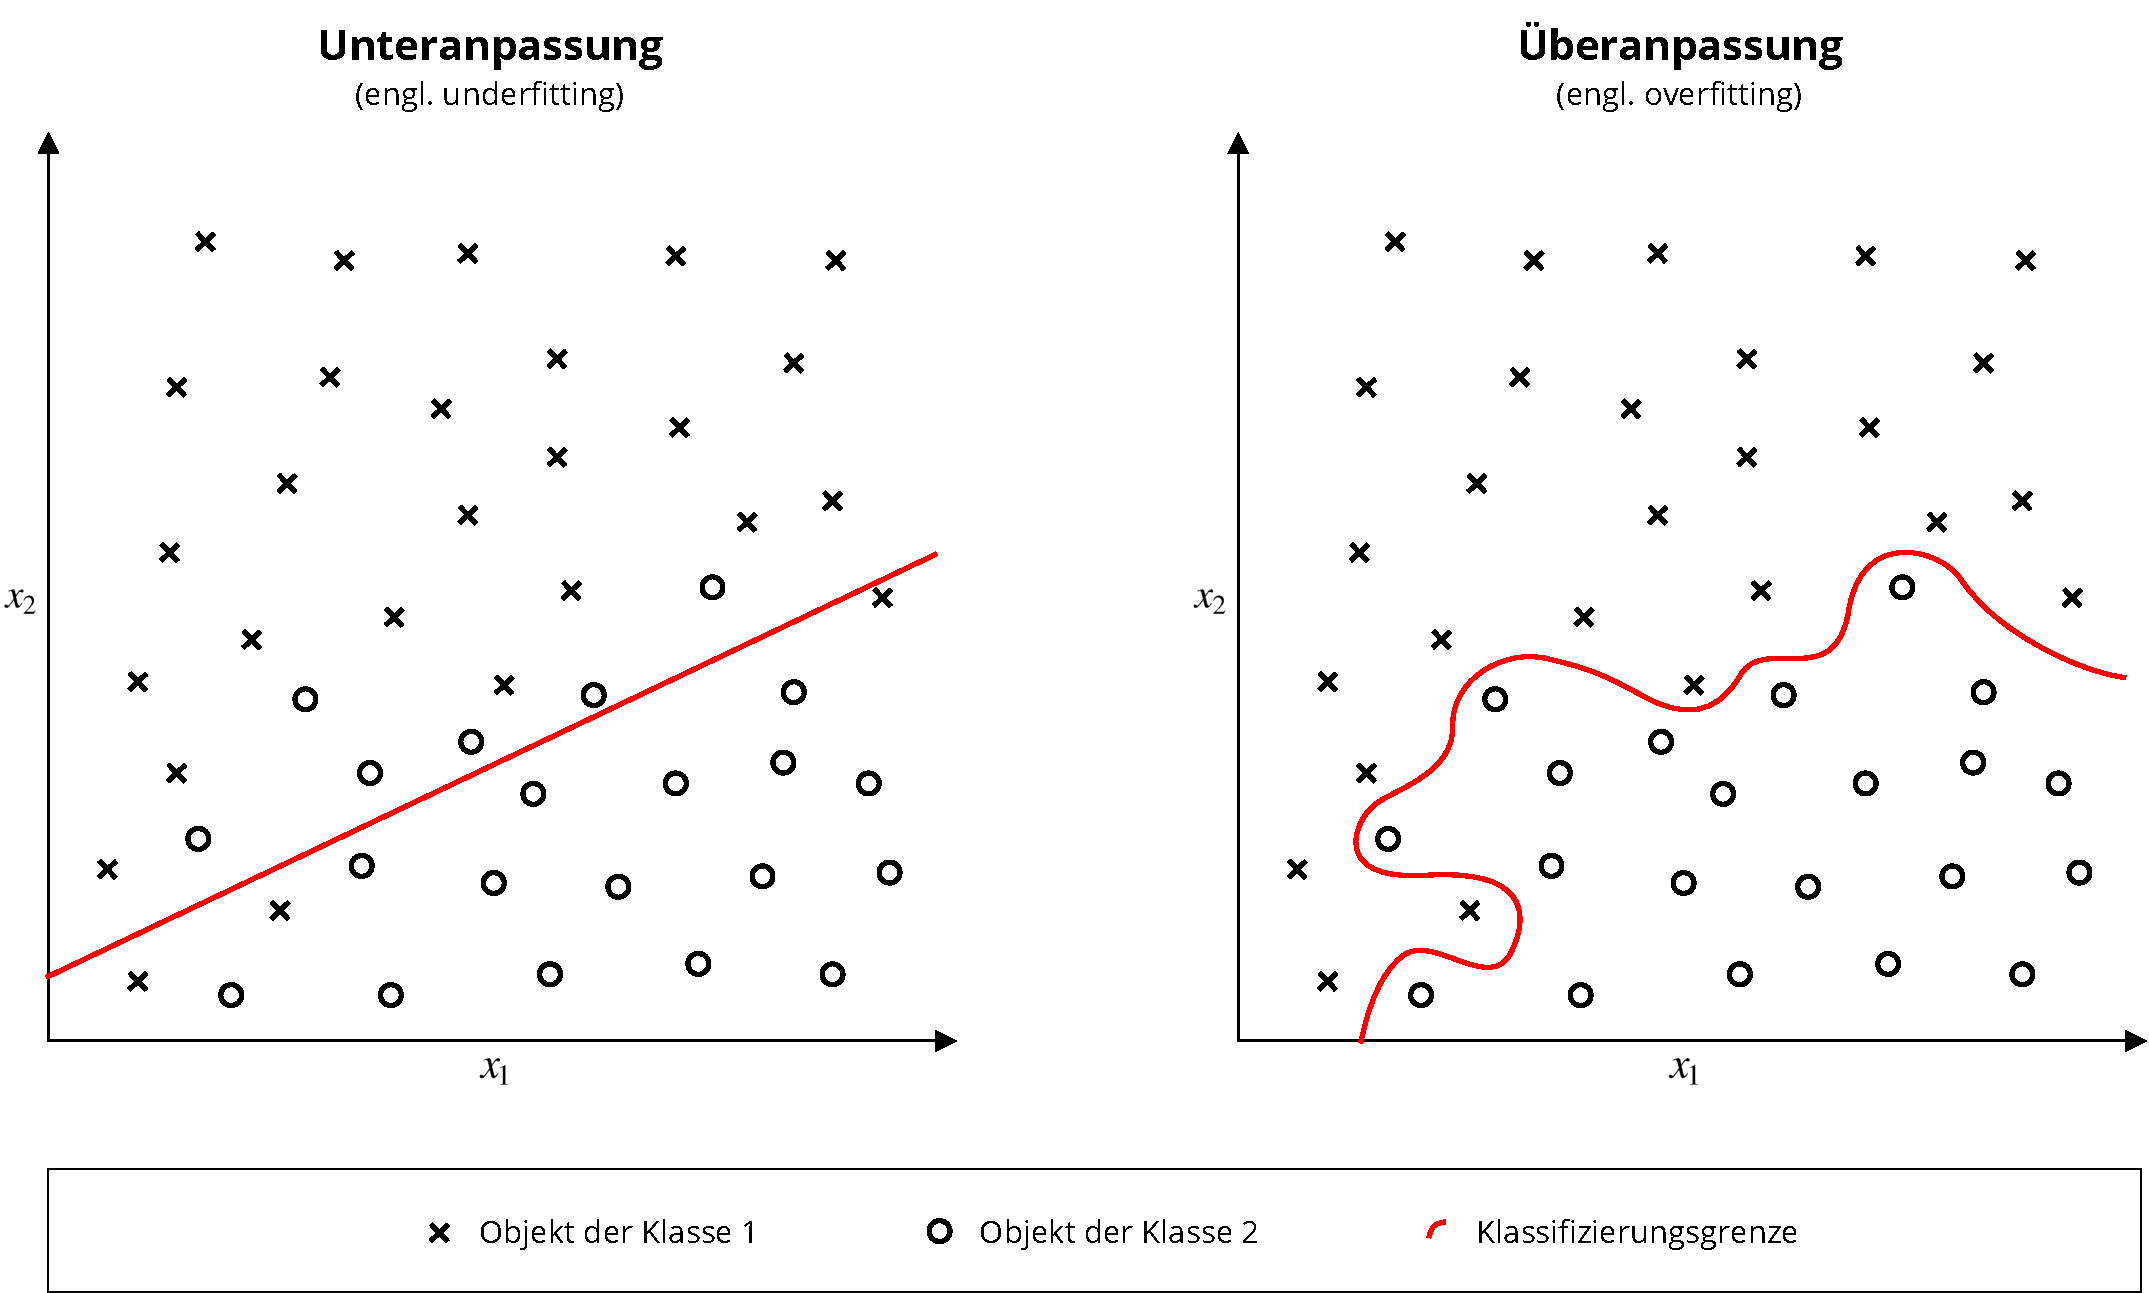
\includegraphics[scale=0.4]{images/overfitting.pdf}
\caption{Beispiel einer Unter- und Überanpassung eines Klassifikators}
\label{fig_overfitting}
\end{figure}

Wenn ein Modell hingegen nur mit den Trainingsdaten gute Ergebnisse erzielt, spricht man von Überanpassung (engl. overfitting). Im Gegensatz dazu spricht man von Unteranpassung (engl. underfitting), wenn ein Modell schon mit den Trainingsdaten sehr schlechte Ergebnisse erzielt. In Abbildung \ref{fig_overfitting} ist beispielhaft eine Unter- und Überanpassung eines binären Klassifikators dargestellt.

Heute werden in Anwendungen häufig tiefe neuronale Netze (engl. deep neural networks) verwendet. Von einem tiefen neuronalen Netz spricht man, wenn es viele versteckte Schichten besitzt. Damit können Merkmale auf verschiedenen Abstraktionsebenen erkannt werden \cite{lecun2015deep}. In den folgenden Absätzen \ref{grundlagen_nn_cnn} und \ref{grundlagen_nn_rnn} werden zwei verschiedene Architekturen von tiefen neuronalen Netzen vorgestellt, die in Kapitel \ref{umsetzung} für das Klassifizierungsproblem dieser Arbeit angewendet werden.


% ===========================
\subsection{Convolutional Neural Networks}
\label{grundlagen_nn_cnn}
% ===========================

Ein \acf{CNN} ist eine Architektur eines \acp{KNN} und gilt heute als Stand der Technik für Probleme in der Bilderkennung \cite{krizhevsky2012imagenet}. Die Architektur eines \acp{CNN} besteht grundsätzlich aus einer oder mehreren Convolution- und Pooling-Schichten \cite{lecun2010convolutional}. Die Abfolge dieser Schichten kann sich beliebig oft wiederholen und wird am Ende mit einer oder mehreren Fully-Connected-Schichten für die Klassifizierung ergänzt. In den folgenden Absätzen werden die Funktionsweisen der Convolution- und der Pooling-Schicht erklärt. Eine Fully-Connected-Schicht entspricht einer Schicht im mehrlagigen Perzeptron wie sie im vorherigen Abschnitt \ref{grundlagen_nn_entwicklung} beschrieben wurde. In Abbildung \ref{fig_cnn} ist ein gesamtes \ac{CNN} dargestellt.

Die Convolution-Schicht besteht aus einer Convolution-Operation gefolgt von einer Aktivierungsfunktion. Die Grundidee dieser Schicht ist die Extraktion von Merkmalen aus einem Bild oder anderen Inputdaten. Dabei werden in den ersten Schichten Merkmale auf einer niedrigen Ebene (engl. low-level features) und in späteren Schichten zunehmend abstraktere Merkmale (engl. high-level features) extrahiert. Bei der Convolution-Operation (oder auch Faltung) wird ein ausgewählter Filter mit einer festgelegten Schrittgröße (engl. stride) über das Bild bewegt und bei jedem Schritt der entsprechende Ausgabewert berechnet \cite{lecun1998cnn}. Diese Operation ist in Abbildung \ref{fig_conv_operation} dargestellt.

\begin{figure}[h]
\centering
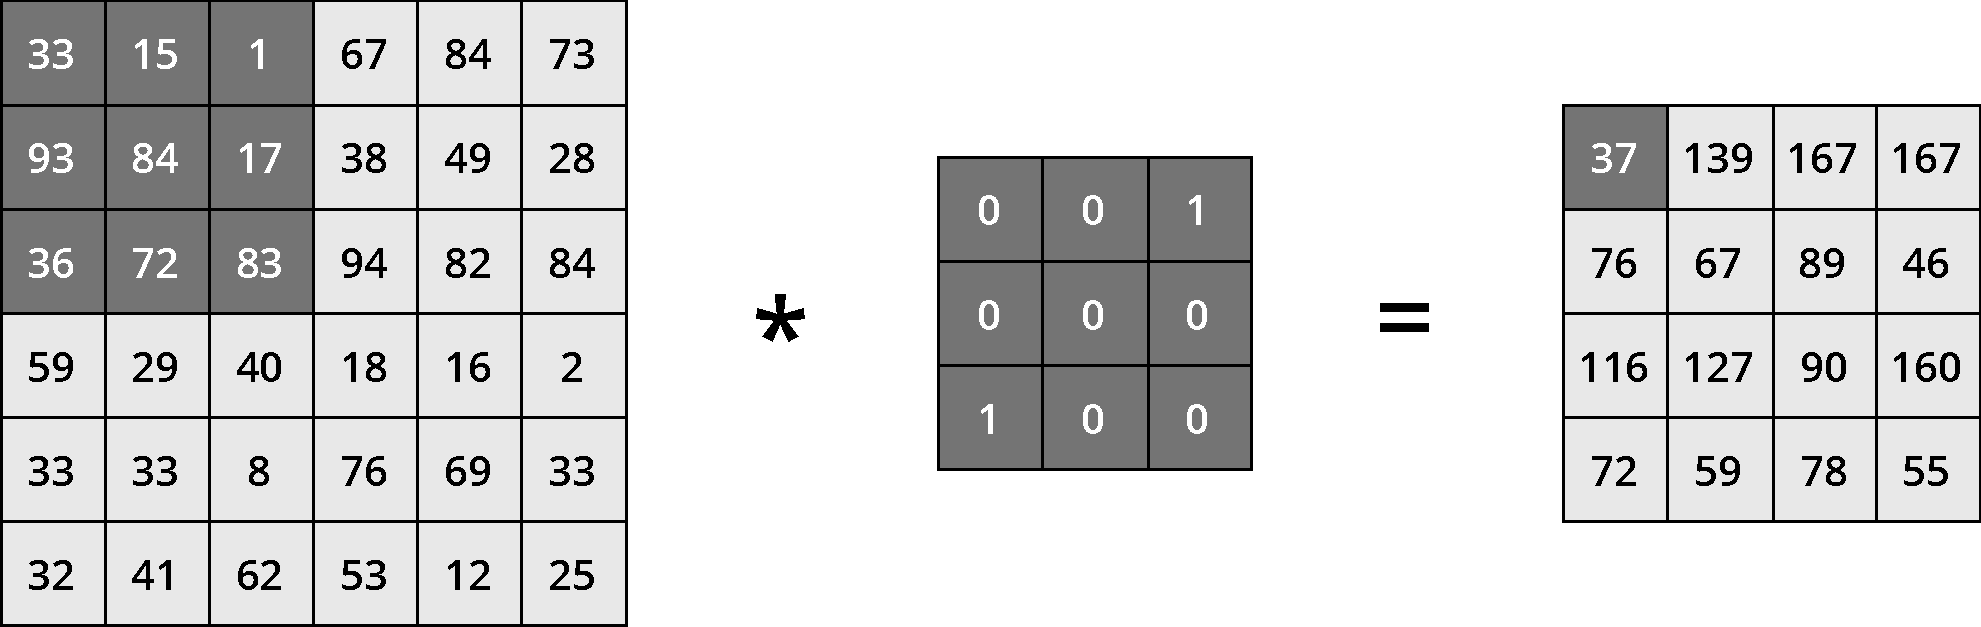
\includegraphics[scale=0.4]{images/conv_operation.pdf}
\caption{Beispiel einer Convolution-Operation}
\label{fig_conv_operation}
\end{figure}

In diesem Beispiel handelt es sich um ein Bild mit den Dimensionen 6 x 6 x 1 Pixel, also einem zweidimensionalen Bild mit einem Farbkanal. Der Filter hat die Dimensionen 3 x 3 x 1. In dem Beispiel ist die aktuell dargestellte Rechnung wie folgt:

\begin{equation*}
0*33+0*15+1*1+0*93+0*84+0*17+1*36+0*72+0*83=37
\end{equation*}

Nach dieser Berechnung bewegt sich der Filter einen Schritt weiter nach rechts und der nächste Wert wird berechnet. Am rechten Rand des Bildes angekommen, wird der Filter eine Schrittlänge weiter nach unten gesetzt und wieder an den linken Rand gesetzt. Dies wiederholt sich bis der Filter am rechten unteren Rand des Bildes angekommen ist. Bei einem dreidimensionalen Bild, mit den drei Farbkanälen als dritte Dimension, hat der Filter ebenfalls drei Dimensionen. Die Berechnung wird analog durchgeführt. Bei dieser Operation kann die Größe des Filters und die Schrittgröße variiert werden. Es können auch verschiedenen Filter verwendet werden, um unterschiedliche Merkmale zu extrahieren. Außerdem können sogenannte Padding-Methoden eingesetzt werden um den Rand der Bilder künstlich zu erweitern. Beim sogenannten Zero-Padding wird beispielsweise ein beliebig breiter Rand mit den Werten 0 um das Bild gelegt. Somit kann sich ein Filter auch über die existierenden Ränder hinweg bewegen und Muster an den Rändern besser erkennen. Das Ergebnis einer Convolution-Schicht ist eine sogenannte Feature Map, also eine Schicht, die aus extrahierten Merkmalen besteht \cite{lecun1997convolutional}.

Das Ziel der Pooling-Schicht ist es, die Größe von Feature Maps zu reduzieren und dabei die wichtigsten Merkmale beizubehalten \cite{scherer2010evaluation}. Wie bei der Convolution-Operation, gibt es auch beim Pooling verschiedene Operationen (z.B. Average-Pooling). In Abbildung \ref{fig_pool_operation} ist die oft verwendete Max-Pooling-Operation dargestellt. Dabei werden Fenster mit einer festgelegten Breite und Höhe über das Bild bewegt und jeweils nur der maximale Wert innerhalb eines Fensters übernommen.

\begin{figure}[h]
\centering
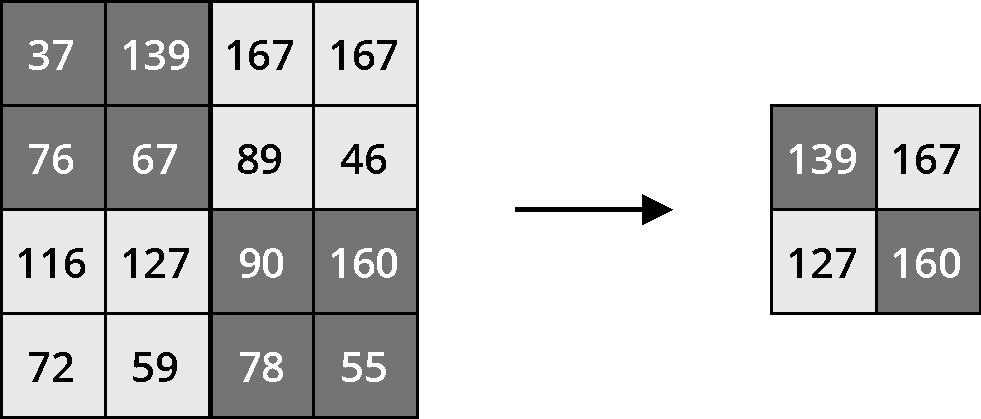
\includegraphics[scale=0.4]{images/pool_operation.pdf}
\caption{Beispiel einer Max-Pooling-Operation}
\label{fig_pool_operation}
\end{figure}

Mit Convolution-, Pooling- und Fully-Connected-Schichten kann die Architektur eines \acp{CNN} zusammengesetzt werden. In Abbildung \ref{fig_cnn} ist beispielhaft die Architektur eines \ac{CNN} abgebildet.


\begin{figure}[h]
\centering
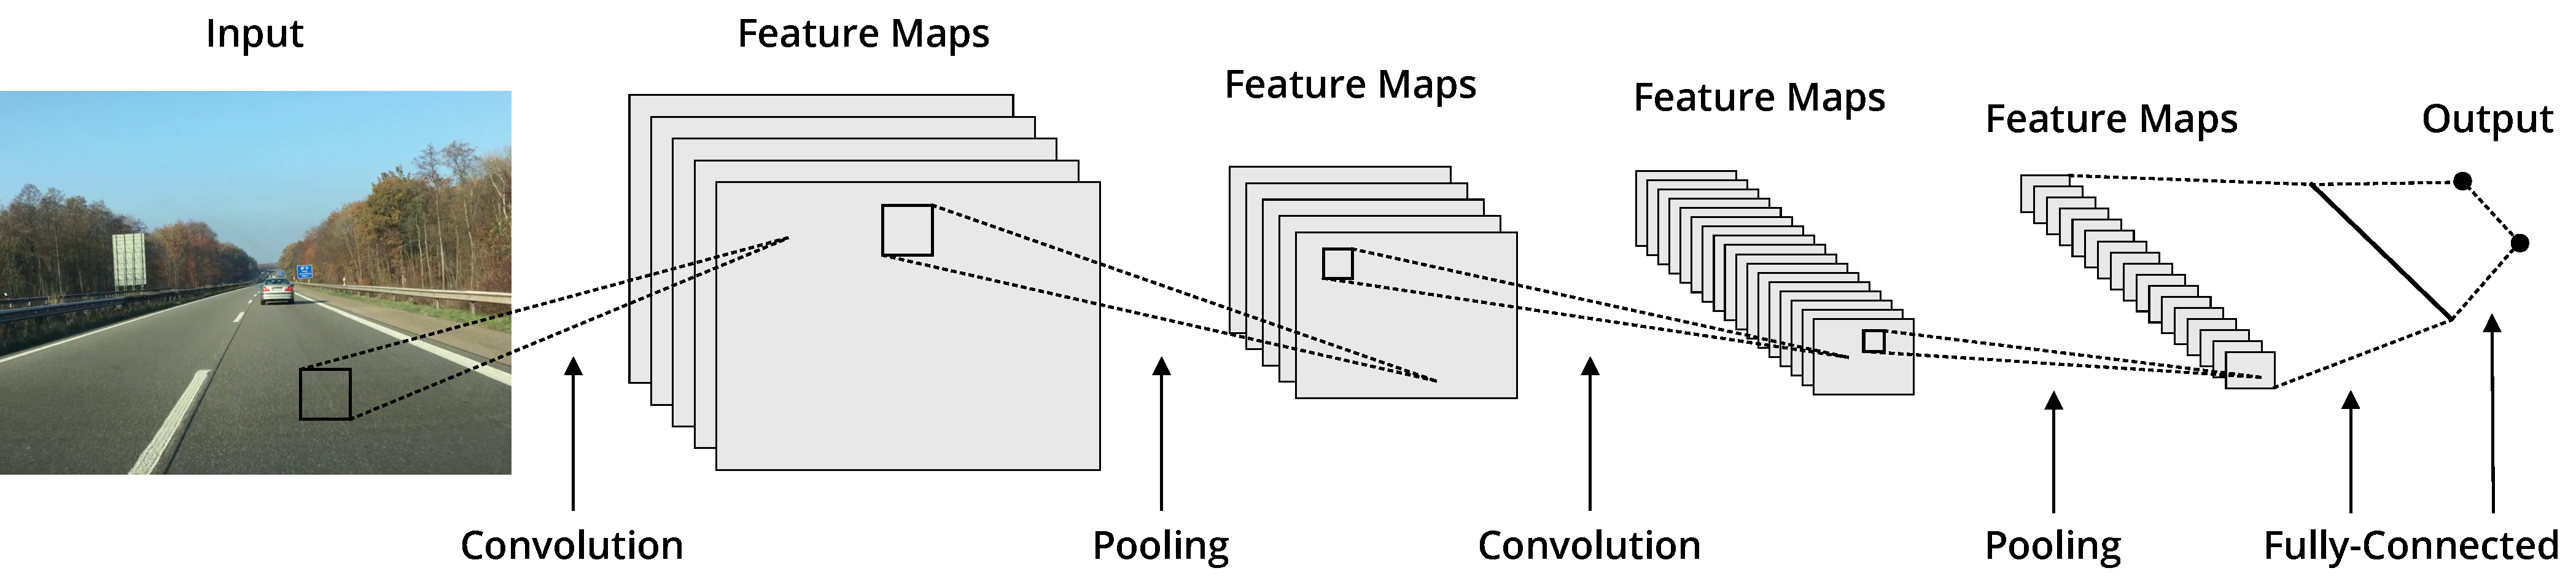
\includegraphics[scale=0.2]{images/cnn.pdf}
\caption{Beispiel eines \aclp{CNN}}
\label{fig_cnn}
\end{figure}


% ===========================
\subsection{Recurrent Neural Networks und LSTMs}
\label{grundlagen_nn_rnn}
% ===========================

In diesem Abschnitt wird die Architektur von \acfp{RNN} und einer modifizierten Version davon, \acfp{LSTM}, vorgestellt. Ein \ac{RNN} ist ein \ac{KNN}, das für sequentielle Daten geeignet ist. Der Unterschied zu der Architektur eines mehrlagigen Perzeptrons ist, dass beim Training auch die Werte von Neuronen derselben Schicht berücksichtigt werden \cite{graves2012rnn}. Damit entsteht nicht nur eine Abhängigkeit zu den Aktivierungswerten der vorherigen Schicht, sondern auch zu den Werten der Neuronen derselben Schicht. Das bedeutet wiederum, dass ein \ac{RNN} nicht von einem einzigen Eingangsvektor abhängig ist, sondern von einer Sequenz von Eingangsvektoren. 

Es gibt verschiedene Architekturen von \acp{RNN}, zum Beispiel mit Ergebniswerten von jedem Input (engl. many to many) oder nur einem Ergebniswert am Ende einer Sequenz (engl. many to one). Die Architekturen mit Ergebniswerten von jedem Input werden beispielsweise für die automatische Übersetzung von Texten verwendet. Dabei ist jeder Input ein neues Wort, für das jeweils ein Ergebnis, wie zum Beispiel eine Übersetzung, produziert wird, und das auch Einfluss auf die Bedeutung der folgenden Wörter hat. Architekturen mit einem Ergebniswert werden für Klassifizierungsprobleme verwendet. Dabei wird einer Sequenz von Inputdaten eine Klasse zugeordnet. Diese beiden Varianten sind schematisch in Abbildung \ref{fig_rnn} dargestellt. In dieser Arbeit wird in Kapitel \ref{umsetzung} die Variante mit einem Ergebnis basierend auf einer Sequenz von Inputdaten verwendet, i.e. die Berechnung einer Klasse auf Basis einer Bildsequenz.

\begin{figure}[h]
\centering
\begin{tabular}{c@{\hskip 1cm}c}
\subfloat[many to many]{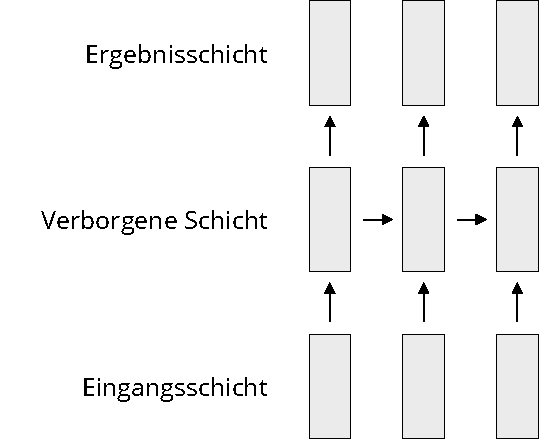
\includegraphics[scale=0.7]{images/rnn_1.pdf}} &
\subfloat[many to one]{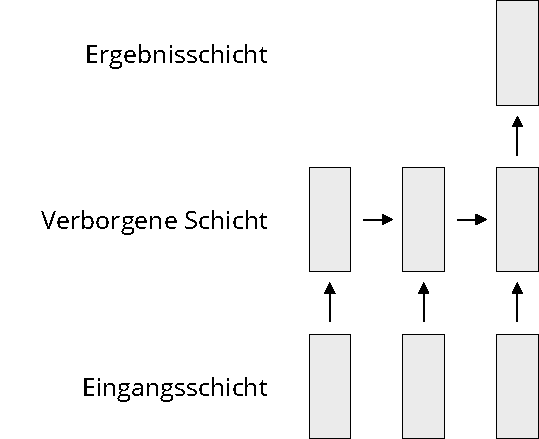
\includegraphics[scale=0.7]{images/rnn_2.pdf}} \\
\end{tabular}
\caption{Beispiel von zwei verschiedenen \acs{RNN}-Architekturen}
\label{fig_rnn}
\end{figure}

Wenn nun in einem \ac{RNN} die Fehlerrückführung (engl. error backpropagation) angewendet wird, kommt es schnell zu dem Problem des verschwindenden oder explodierenden Gradienten (engl. vanishing or exploding gradient). Das basiert auf der Multiplikation der Gradienten von mehreren Sequenzschritten. Wenn der Gradient größer als 1 ist, wächst er sehr stark (explodiert), wenn er kleiner als 1 ist, geht er schnell gegen 0 (verschwindet). In beiden Fällen kann es zu sehr langen Trainingszeiten, in Extremfällen zu keinem Lerneffekt während des Trainings, kommen \cite{graves2012rnn}. Die Lösung dieses Problems wurde von Hochreiter und Schmidhuber \cite{hochreiter1997long} in Form der \ac{LSTM}-Zelle vorgestellt.

Eine \ac{LSTM}-Zelle ist mit drei Toren, dem Eingangstor (engl. input gate), dem Merk- und Vergesstor (engl. forget gate) und dem Ausgangstor (engl. output gate), und einem Zellenzustand aufgebaut. Die Idee ist, dass die \ac{LSTM}-Zelle einen Zustand speichern und damit erhalten kann. Das verhindert den Effekt des verschwindenden oder explodierenden Gradienten. Die Abbildung \ref{fig_lstm} zeigt eine solche \ac{LSTM}-Zelle.

\begin{figure}[h]
\centering
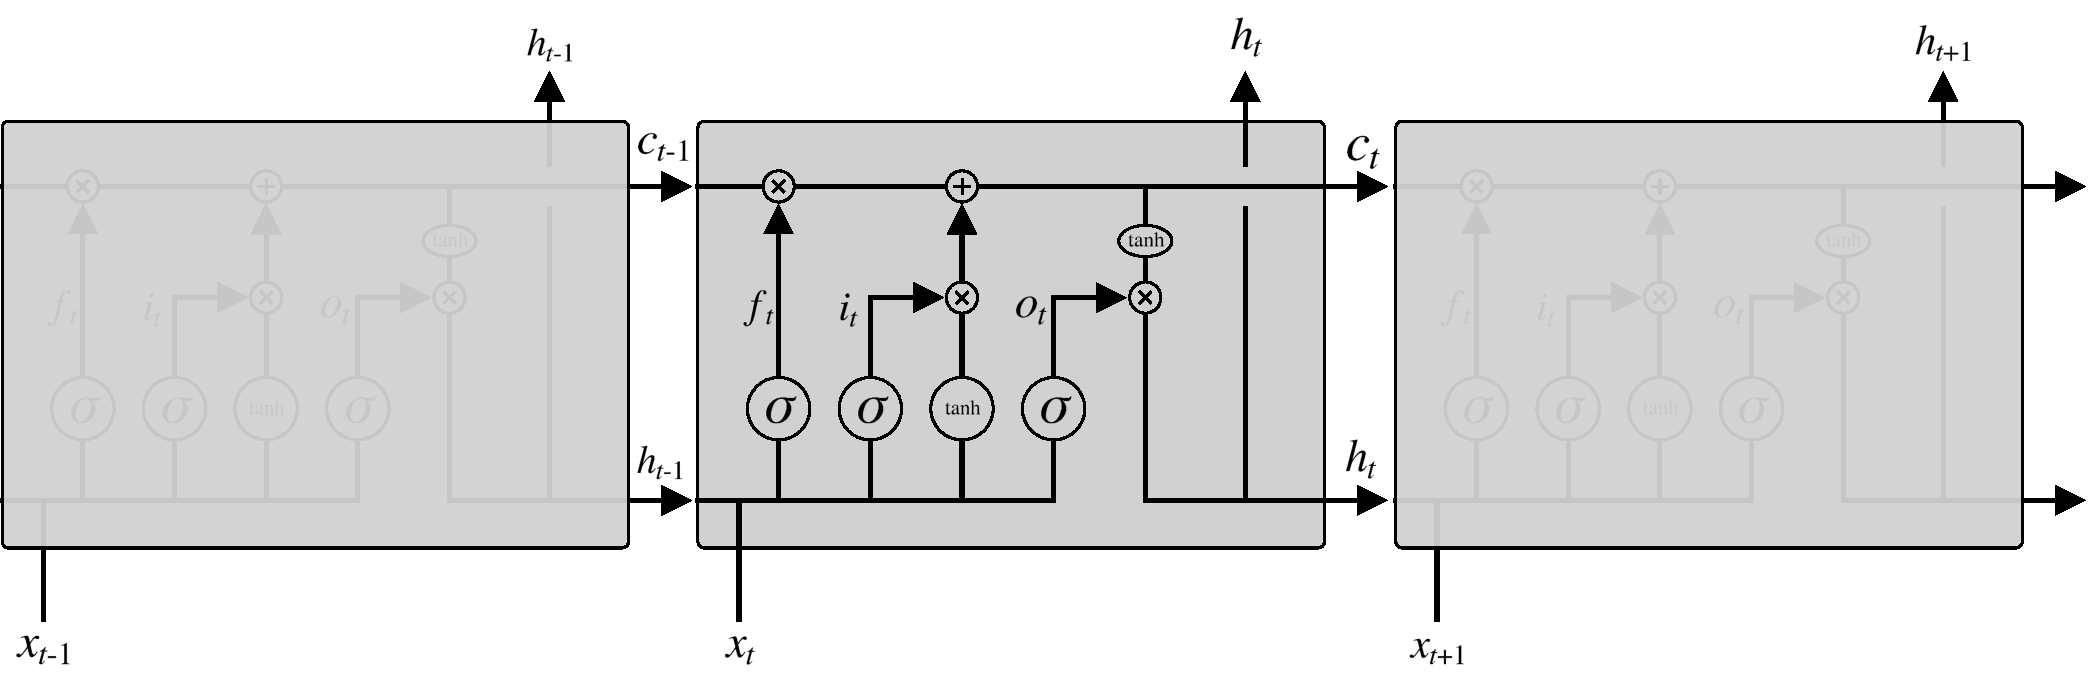
\includegraphics[scale=0.4]{images/lstm.pdf}
\caption[\acl{LSTM}-Zelle]{\acl{LSTM}-Zelle \cite{olah2015lstm}}
\label{fig_lstm}
\end{figure}

Das Vergesstor $f_t$, das Eingangstor $i_t$ und das Ausgangstor $o_t$ ist jeweils mit einer Sigmoid-Funktion $\sigma$ modelliert und hat als Ergebnis einen Wert zwischen 0 und 1. Dieser Wert gibt an, wie durchlässig das jeweilige Tor ist. Der Zustand der Zelle $c_t$ zum Zeitpunkt $t$ wird von der Zelle verwendet, um Werte zu speichern oder zu ändern. $x_t$ ist der Dateninput zum Zeitpunkt $t$. Die Tore $f_t$, $i_t$ und $o_t$, der Zustand der Zelle $c_t$ und der Ergebniswert $h_t$ der Zelle werden mit der jeweiligen Gewichtsmatrix $W$ und dem Bias $b$ wie folgt berechnet \cite{olah2015lstm}.

\begin{equation}
f_t = \sigma (W_f[h_{t-1}, x_t] + b_f)
\end{equation}

\begin{equation}
i_t = \sigma (W_i[h_{t-1}, x_t] + b_i)
\end{equation}

\begin{equation}
o_t = \sigma (W_o[h_{t-1}, x_t] + b_o)
\end{equation}

\begin{equation}
c_t = f_t * c_{t-1} + i_t * \tanh((W_c[h_{t-1}, x_t]) + b_c)
\end{equation}

\begin{equation}
h_t = o_t * \tanh(c_t)
\end{equation}


% ===========================
\subsection{Training mit synthetischen Daten}
\label{grundlagen_nn_synthetisch}
% ===========================

Ein großes Problem beim Training von neuronalen Netzen ist der manuelle Aufwand um reale Trainings- und Validierungsdaten zu annotieren \cite{richter2016playing}. Ein Ansatz dem entgegenzuwirken ist das Training mit synthetischen Daten oder einer Kombination aus synthetischen und realen Daten. In diesem Abschnitt werden vier Arbeiten aus den letzten Jahren vorgestellt, die diesen Ansatz untersuchen. Die Datensätze dieser Arbeiten werden im Abschnitt \ref{umsetzung_daten_real} in Tabelle \ref{tab_datensaetze} zusammengefasst und mit dem Datensatz aus dieser Arbeit verglichen.

Ros et al. \cite{ros2016synthia} haben für die Simulation einer virtuellen Stadt die Unity Development Platform verwendet. Mit virtuellen Fahrten wurden insgesamt circa 200.000 Bilder generiert und diese mit 11 Klassen (e.g. \textit{Sky, Buildings, Road}) auf Pixelebene annotiert. Für das Training wurden die Bilder auf eine Größe von 180 x 120 Pixel reduziert. Das kombinierte Training mit synthetischen und realen Daten auf den Datensätzen KITTI, CamVid, U-LabelMe und CBCL hat die Genauigkeit (engl. accuracy) auf den realen Testdaten, im Vergleich zum Training mit ausschließlich realen Daten, deutlich gesteigert.

Johnson-Roberson et al. \cite{johnson2017driving} und Richter et al. \cite{richter2016playing} haben für die Generierung von Trainingsdaten das Computerspiel Grand Theft Auto V verwendet. Die Grafikleistung dieses Spiels übertrifft kommerzielle und Open-Source Simulationssoftware und ist daher sehr gut für die Simulation von Bilddaten geeignet. Johnson-Roberson et al. \cite{johnson2017driving} generierten zwei Datensätze mit 50.000 und 200.000 Bildern mit Begrenzungsboxen (engl. bounding boxes) für Fahrzeuge. Mit ihrem kombinierten Training zusammen mit dem KITTI Datensatz konnten sie die Genauigkeit auf den Testdaten, im Vergleich zum Training auf ausschließlich realen Daten, verbessern. Richter et al. \cite{richter2016playing} generierten 25.000 Bilder mit einer Annotation auf Pixelebene von 19 Klassen (e.g. \textit{Road, Sky, Car}). Mit diesen Bildern und einem kombinierten Training zusammen mit dem KITTI Datensatz konnten auch sie die Genauigkeit verbessern.

Tremblay et al. \cite{tremblay2018training} verfolgten bei der Generierung von Bildern einen anderen Ansatz. Sie nutzten 3D Modelle von Fahrzeugen und platzierten diese mit zufälliger Position und Ausrichtungen auf verschiedenen realen Szenen. Die 100.000 Bilder wurden mit Begrenzungsboxen (engl. bounding boxes) annotiert. Beim Training wurden ausschließlich die synthetischen Daten verwendet und es wurde eine Genauigkeit von circa 80 Prozent erreicht.

Generell zeigt das Training von neuronalen Netzen mit einer Kombination von synthetischen und realen Daten bereits vielversprechende Ergebnisse, auf denen dieses Arbeit aufbauen will. Im Gegensatz zu den vergangenen Arbeiten, werden in dieser Arbeit ganze Szenarien generiert und annotiert und nicht einzelne Bilder mit Begrenzungsboxen oder semantischer Annotation auf Pixelebene.


% ===========================
\subsection{Klassifizierung von Videos}
\label{grundlagen_nn_video}
% ===========================

Grundsätzlich kann zwischen drei verschiedenen Ansätzen bei der Klassifizierung von Videos mit \acp{KNN} unterschieden werden. Beim ersten Ansatz werden die einzelnen Bilder aus einem Video mit einem \ac{CNN} klassifiziert und anschließend wird das Video der Klasse zugeordnet, zu der die meisten Bilder zugeordnet wurden \cite{karpathy2014large}. Mit diesem Ansatz werden die räumlichen Merkmale (engl. spatial features) mit dem \ac{CNN} sehr gut extrahiert und bei der Klassifizierung berücksichtigt. Das Problem ist, dass zeitliche Merkmale (engl. temporal features) keine Beachtung finden und die Reihenfolge der einzelnen Bilder ignoriert wird. Dieser Ansatz ist in Abbildung \ref{fig_single_frame_classification} dargestellt.

\begin{figure}[h]
\centering
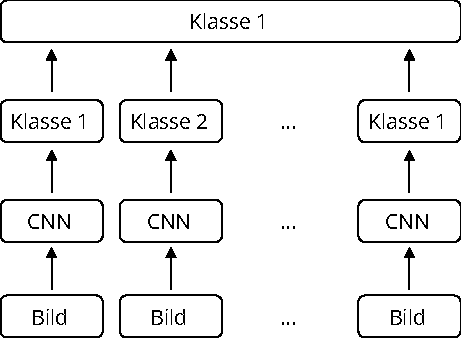
\includegraphics[scale=0.8]{images/single_frame_classification.pdf}
\caption{Klassifizierung von einzelnen Bildern mit anschließender Klassifizierung des gesamten Videos}
\label{fig_single_frame_classification}
\end{figure}

Ein weiterer Ansatz basiert auf der Idee, Feature Maps von mehreren Bildern zu kombinieren und damit die zeitlichen Merkmalen mit 3D-Filtern eines \acp{CNN} zu extrahieren. In früheren Arbeiten wurde für diese Kombination eine Pooling-Operation verwendet \cite{karpathy2014large, yue2015beyond} und es wurden verschiedene Architekturen mit früher, später oder langsamer Fusion verwendet (engl. early, late, and slow fusion). Bei der frühen Fusion werden schon zu Beginn die Eingangswerte von mehreren Bildern kombiniert. Bei der späten Fusion werden von allen Bildern Merkmale extrahiert und am Ende mit einer Pooling-Schicht vereint. Beim Ansatz der langsamen Fusion werden schrittweise die Feature Maps von immer mehr Bildern zusammengefasst. Diese Architekturen sind schematisch in Abbildung \ref{fig_fusion_classification} dargestellt.

\begin{figure}[h]
\centering
\begin{tabular}{c@{\hskip 0.7cm}c@{\hskip 0.7cm}c}
\subfloat[Frühe Fusion]{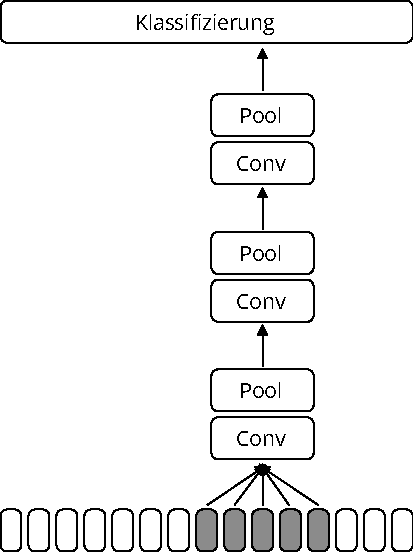
\includegraphics[scale=0.6]{images/fusion_early.pdf}} &
\subfloat[Späte Fusion]{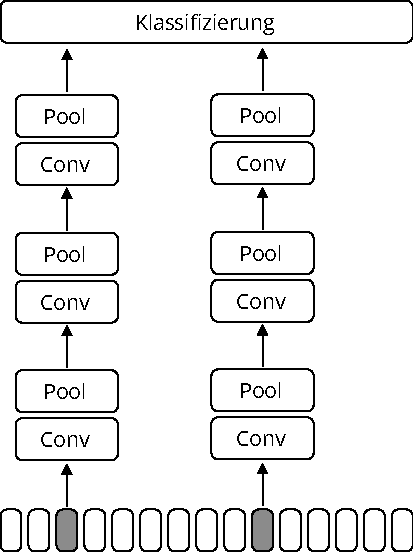
\includegraphics[scale=0.6]{images/fusion_late.pdf}} &
\subfloat[Langsame Fusion]{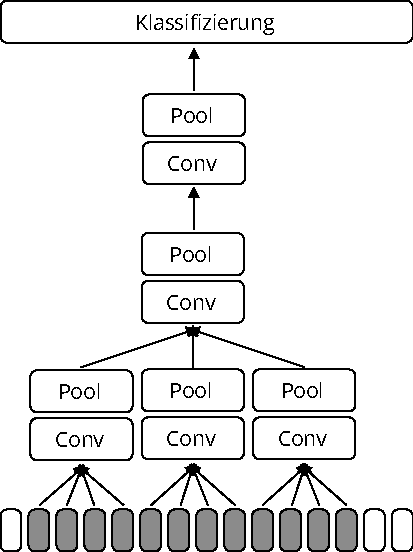
\includegraphics[scale=0.6]{images/fusion_slow.pdf}} 
\end{tabular}
\caption[Schematische Darstellung von Klassifizierungsarchitekturen mit frühen, späten und langsamen Fusionen von Feature Maps]{Schematische Darstellung von Klassifizierungsarchitekturen mit frühen, späten und langsamen Fusionen von Feature Maps \cite{karpathy2014large}}
\label{fig_fusion_classification}
\end{figure}

Später wurden neben der Pooling-Operation andere Operationen für die Fusion entwickelt \cite{feichtenhofer2016convolutional}. Obwohl damit teilweise sehr gute Ergebnisse erzielt werden konnten \cite{carreira2017quo}, haben die Fusions-Architekturen einen entscheidenden Nachteil. Zeitliche Merkmale werden berücksichtigt, allerdings nicht die Reihenfolge der Bilder. Aus diesem Grund gibt es einen dritten Ansatz für die Klassifizierung von Videos, die Kombination aus \acp{CNN}, die räumliche Merkmale extrahieren, und \acp{LSTM}, die zeitliche Merkmale extrahieren. Eine Architektur mit diesem Ansatz wurde von Donahue et al. \cite{donahue2015long} vorgestellt. Dabei wird ein vortrainiertes \ac{CNN} verwendet, um die räumlichen Merkmale aus allen Bildern zu extrahieren. Anschließend werden diese Feature Maps einer \ac{LSTM}-Schicht übergeben, welche die zeitlichen Merkmale extrahiert. In Abbildung \ref{fig_cnn_lstm_architektur} ist diese Architektur schematisch dargestellt.

\begin{figure}[h]
\centering
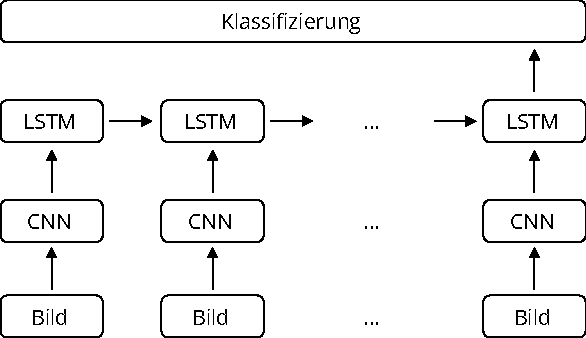
\includegraphics[scale=0.8]{images/cnn_lstm_architektur.pdf}
\caption[Klassifizierung von Videos mit einer \acs{CNN}-\acs{LSTM}-Architektur]{Klassifizierung von Videos mit einer \acs{CNN}-\acs{LSTM}-Architektur \cite{donahue2015long}}
\label{fig_cnn_lstm_architektur}
\end{figure}

In dieser Arbeit wird der erste Ansatz, die Klassifizierung von einzelnen Bilder mit anschließender Klassifizierung des gesamten Videos, und der dritte Ansatz, die kombinierte \ac{CNN}-\ac{LSTM}-Architektur verwendet. Die Architekturen dieser Arbeit werden im Detail in Abschnitt \ref{umsetzung_training_architektur} vorgestellt.




% ===========================
\chapter{Konzept}
\label{konzept}
% ===========================

Wie in Abschnitt \ref{grundlagen_fahren} beschrieben, stellt die Absicherung von hochautomatisierten \ac{FAS} die Automobilindustrie vor große Herausforderungen. Die Menge der bekannten Fahrszenarien ist nur eine Teilmenge aller Szenarien, die zukünftige \ac{FAS} abdecken müssen. Die Folge ist eine steigende Anzahl benötigter Testkilometer, die in Zukunft mit ökonomischem Aufwand nicht mehr umsetzbar sein wird. Es müssen neue Methoden gefunden werden, relevante Szenarien für die Generierung von Testfällen zu identifizieren, um die Sicherung von hochautomatisierten \ac{FAS} mit ökonomischen Aufwand garantieren zu können.

Genau hier soll diese Arbeit einen Beitrag leisten. Das Ziel, wie bereits in Abschnitt \ref{einleitung_zielsetzung} erklärt, ist die Klassifizierung von realen Fahrszenarien. Die Grundidee ist es, einen Klassifikator mit einem großen Anteil synthetischer Daten und einem kleinen Anteil realer Daten von bisher bekannten Szenarien zu trainieren. Es wird mit einem großen Teil synthetischer Daten gearbeitet, weil es in der Praxis einfacher ist, synthetische Daten zu generieren und automatisch zu annotieren als große Mengen realer Daten zu annotieren. Der trainierte Klassifikator kann dann bekannte Szenarien erkennen. Die Idee ist, dass auf diese Weise auch unbekannte Szenarien herausgefiltert werden können, weil diese von dem trainierten Klassifikator nicht erkannt werden. Diese bisher unbekannten Szenarien können dann wiederum als Basis für neue Testfälle für die Sicherung hochautomatisierter Fahrfunktionen verwendet werden.

In dieser Arbeit soll ein Proof-of-Concept für diese Methodik entwickelt werden. Dafür wird im folgenden Abschnitt \ref{konzept_struktur} das Konzept im Detail und die Vorgehensweise vorgestellt. Anschließend wird in Abschnitt \ref{konzept_methodik} die Methodik erklärt, mit welcher dieses Konzept umgesetzt werden soll.


% ===========================
\section{Struktur}
\label{konzept_struktur}
% ===========================

Das Konzept dieser Arbeit lässt sich in vier Teile untergliedern. Im ersten Teil werden beispielhaft einige Szenarien ausgewählt und auf der Ebene der \textit{logischen Szenarien} definiert. Auf dieser Basis werden im zweiten Teil synthetische und reale Trainingsdaten generiert. Im dritten Teil wird ein \ac{KNN} als Klassifikator trainiert und evaluiert. Anschließend können diese Schritte mit allen bekannten Szenarien wiederholt werden um bisher unebkannte Szenarien zu finden. Die ersten drei Schritte, die in dieser Arbeit als Proof-of-Concept umgesetzt werden, ist schematisch in Abbildung \ref{fig_konzept_struktur} dargestellt. In den folgenden Absätzen werden die Schritte im Detail beschrieben.

\begin{figure}[h]
\centering
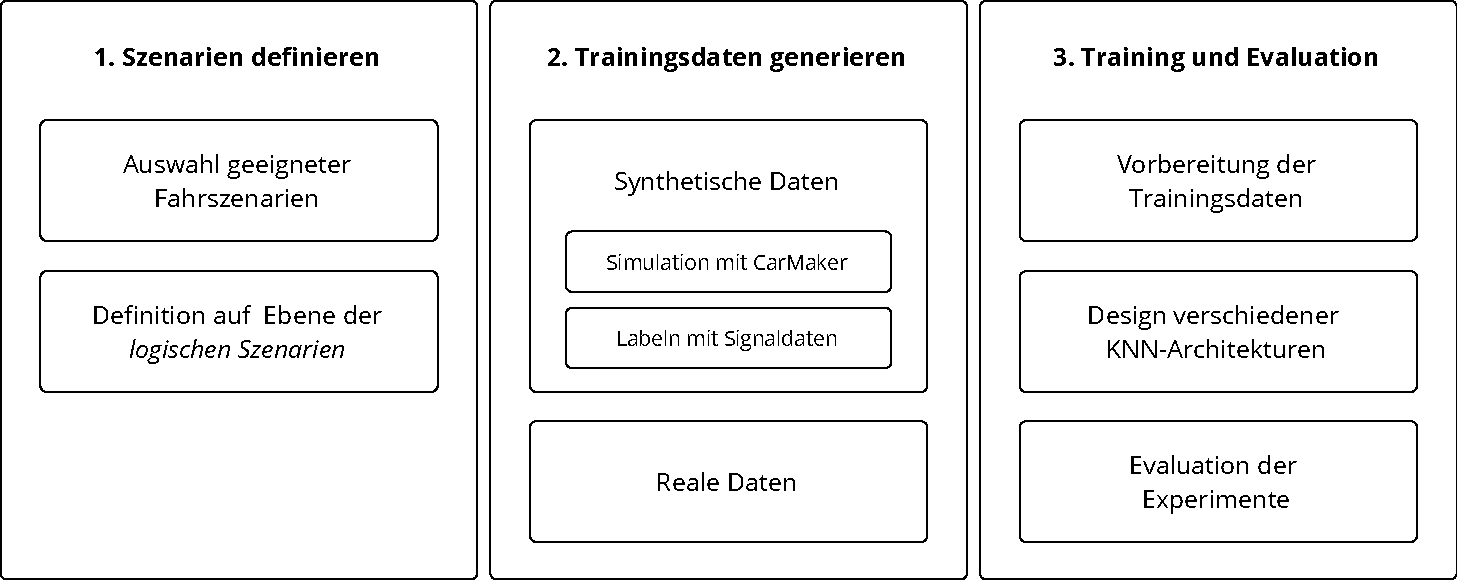
\includegraphics[scale=0.6]{images/konzept_struktur.pdf}
\caption{Konzept dieser Arbeit}
\label{fig_konzept_struktur}
\end{figure}

Im ersten Schritt werden beispielhaft Fahrszenarien ausgewählt und wie in Abschnitt \ref{grundlagen_fahren_szenarien} definiert. In dieser Arbeit werden Szenarien auf der Ebene der \textit{logischen Szenarien} definiert. Nachdem Szenarien ausgewählt und definiert sind, werden synthetische und reale Daten für das Training eines Klassifikators benötigt.

Für die Generierung von synthetischen Daten wird mit einer Simulationssoftware gearbeitet. Die Idee ist es, Fahrten eines Ego-Fahrzeugs zu simulieren, entsprechende Bild- und Signaldaten aufzuzeichnen und die Bilddaten anhand der Signaldaten zu annotieren. Auf diese Weise können ohne großen Aufwand beliebig viele synthetische Daten erzeugt und annotiert werden. Amersbach und Winner \cite{amersbach2017functional} stellen einen Ansatz für die funktionale Dekomposition von hochautomatisierten \ac{FAS} vor. In diesem Ansatz werden Informationen über sechs Schichten, von den Ground Truth Daten über die Szenenerkennung bis zur entsprechenden Aktion des Ego-Fahrzeugs, abgeleitet. Ein Schema dieses Ansatzes ist in Abbildung \ref{fig_functional_decomposition} dargestellt. In dieser Arbeit werden für die Annotation der Bilddaten Signaldaten generiert, die nach Schicht 1 (e.g. Geschwindigkeit des Ego-Fahrzeugs) und Schicht 2 (e.g Position des vorausfahrenden Fahrzeugs) eingeordnet werden können. Jeder generierte Zeitpunkt stellt eine Szene, wie in Abschnitt \ref{grundlagen_fahren_szenarien} beschrieben, dar. Jede Szene wird separat auf Basis der entsprechenden Signaldaten nach festgelegten Regeln klassifiziert. Die Aneinanderreihung von mehreren Szenen ergibt schließlich ein Szenario. Für die Generierung von realen Trainingsdaten werden aufgezeichnete Videos verwendet und manuell annotiert.

\begin{figure}[h]
\centering
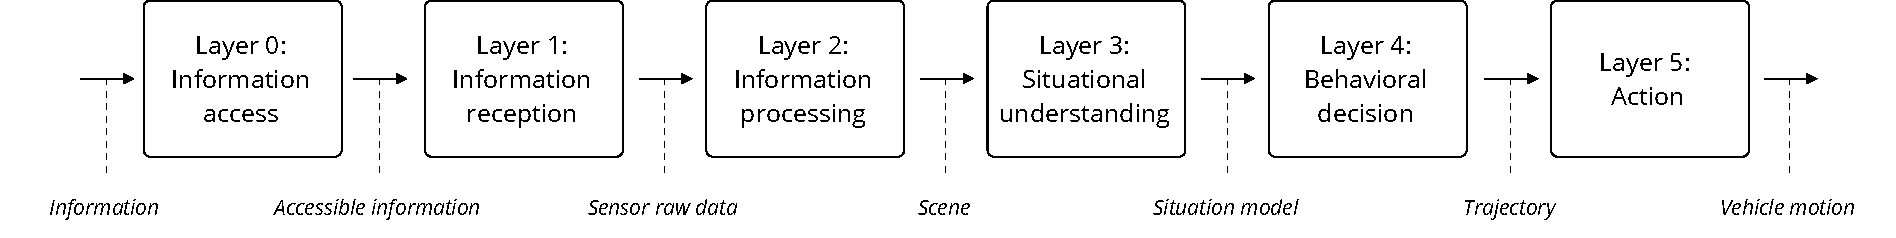
\includegraphics[scale=0.45]{images/funktionale_dekomposition.pdf}
\caption[Schema der funktionalen Dekomposition]{Schema der funktionalen Dekomposition \cite{amersbach2017functional}}
\label{fig_functional_decomposition}
\end{figure}

Für das Training und die Evaluation eines Klassifikatorssollen \acp{KNN} verwendet werden. Wie in Abschnitt \ref{grundlagen_nn_video} beschrieben, gibt es verschiedene Ansätze wie ein Klassifikator für Videos trainiert werden kann. In dieser Arbeit werden zwei verschiedene Ansätze angewendet und miteinander verglichen. Beim ersten Ansatz werden \acp{CNN} verwendet, um einzelne Bilder zu klassifizieren. \acp{CNN} sind nach dem Stand der Technik die besten Architekturen um Merkmale aus Bildern zu extrahieren. Im Anschluss werden Videos der Klasse zugeordnet, zu der auch die meisten Bilder im Video zugeordnet wurden. Mit dem zweiten Ansatz wird ein Klassifikator aus einer Kombination von \acp{CNN} und \acp{LSTM} erstellt. Damit können räumliche und zeitliche Merkmale aus Videos extrahiert und  dann klassifiziert werden. Wie oben beschrieben wird für das Training nur ein kleiner Teil realer und ein großer Teil synthetischer Daten verwendet, um die Skalierbarkeit dieses Ansatzes in der Praxis zu gewährleisten.

Der Proof-of-Concept in dieser Arbeit ist erfolgreich, wenn ein Klassifikator mit diesen drei Schritte trainiert wird und im Anschluss Szenarien auf Basis von Bilddaten klassifizieren kann. Danach kann in einem vierten Schritt ein weiterer Klassifikator mit allen bisher bekannten Szenarien nach demselben Prinzip trainiert werden. Dieser Klassifikator kann dann alle bisher bekannten Szenarien klassifizieren und bisher unbekannte Szenarien herausfiltern, wenn beispielsweise eine Schwelle für die Klassifizierungsgenauigkeit unterschritten wird. Damit wird es möglich die Menge der bisher bekannten Szenarien zu erweitern und schließlich die Absicherung von hochautomatisierten \ac{FAS} weiter voranzutreiben.

% ===========================
\section{Ansätze, Methoden, Werkzeuge}
\label{konzept_methodik}
% ===========================

In diesem Abschnitt wird ein Überblick gegeben, welche Ansätze, Methoden und Werkzeuge in den jeweiligen Teilen der Umsetzung verwendet werden. Diese Zuordnung ist in der folgenden Tabelle \ref{tab_konzept_methods} dargestellt. Die detaillierte Beschreibung folgt in Kapitel \ref{umsetzung}.

\begin{longtable}[c]{p{5cm} p{6.5cm} p{1.5cm}}
\textbf{Teil der Umsetzung} & \textbf{Ansätze, Methoden, Werkzeuge} & \textbf{Quellen} \\
\hline
\endhead

Auswahl und Definition geeigneter Fahrszenarien & Konzept der \textit{logischen Szenarien} & \cite{ulbrich2015defining}, \cite{bagschik2017szenarien} \\
\hline
Simulation und Annotation synthetischer Trainingsdaten & Generierung von Bild- und Signaldaten mit CarMaker, regelbasierte Klassifizierung auf Basis von vorher festgelegten Signaldaten & \cite{ipg2018carmaker} \\
\hline
Generierung realer Trainingsdaten & Auswahl geeigneter Videosequenzen von YouTube, manuelle Annotation & \cite{youtube2018video}, \cite{google2018route1}, \cite{google2018route2} \\
\hline
Vorbereitung der Daten, Erstellung des Klassifikators und Evaluation der Experimente & Verschiedene Architekturen mit \acp{CNN} und \acp{LSTM}, implementiert mit Python und Keras & \cite{chollet2015keras}, \cite{lecun2010convolutional}, \cite{hochreiter1997long} \\

\hline
\caption{Ansätze, Methoden und Werkzeuge dieser Arbeit}
\label{tab_konzept_methods}
\end{longtable}





 

% ===========================
\chapter{Umsetzung}
\label{umsetzung}
% ===========================

In diesem Kapitel wird die Umsetzung des Konzepts aus dem vorherigen Kapitel beschrieben. Zu Beginn werden die dafür notwendigen Fahrszenarien in Abschnitt \ref{umsetzung_definition} definiert. Danach wirda in den Abschnitten \ref{umsetzung_daten_synth} und \ref{umsetzung_daten_real} die Methodik für die Generierung von synthetische Trainingsdaten und reale Trainings- und Testdaten erläutert. Im Anschluss wird in Abschnitt \ref{umsetzung_training} die Architektur und die Experimente des Klassifikators für die Szenarienerkennung beschrieben.


% ===========================
\section{Definition der Fahrszenarien}
\label{umsetzung_definition}
% ===========================

In diesem Abschnitt werden Szenarien, wie in Abschnitt \ref{grundlagen_fahren_szenarien} beschrieben, als \textit{logische Szenarien} für das weitere Vorgehen in dieser Arbeit definiert. In Anlehnung an bestehende Arbeiten zu Erkennung von Fahrszenarien und auf Basis von Machbarkeitsabschätzungen für die Umsetzung werden in dieser Arbeit die Szenarien \textit{free cruising}, \textit{approaching} \textit{following}, \textit{catching up}, \textit{overtaking}, \textit{lane change left} und \textit{lane change right} auf der Autobahn betrachtet. Die Autobahn wurde ausgewählt, weil es weniger Parameter zu betrachten gibt als auf anderen Straßen wie beispielsweise in der Stadt. In der folgenden Tabelle \ref{tab_definition_szenarios} werden diese Szenarien auf \textit{funktionaler} und \textit{logischer Ebene} definiert.

Um die Darstellung in der Tabelle zu erleichtern werden folgende Abstände zwischen Ego-Fahrzeug und Fahrzeug 2 definiert. Dabei beschreibt $ego_v$ die Geschwindigkeit des Ego-Fahrzeugs in [m/s].

\begin{equation*}
\begin{split}
s_0 = ego_v * 3,6 \qquad \text{[m]} \\
s_1 = ego_v * 3,6 * \frac{2}{3} \qquad \text{[m]} \\
s_2 = ego_v * 3,6 * \frac{1}{2} \qquad \text{[m]} \\
s_3 = ego_v * 3,6 * \frac{1}{3} \qquad \text{[m]} \\
\end{split}
\end{equation*}

\small
\begin{longtable}[c]{p{2cm} p{5.5cm} p{6cm}}
\textbf{Szenario} & \textbf{Funktionale Definition} & \textbf{Logische Definition} \\
\hline
\endhead

\textbf{Alle} & 2-spurige Autobahn geradeaus oder in einer Kurve, Geschwindigkeitsbegrenzung ist größer als 80 km/h & Breite Fahrstreifen [2,3..3,5] m \newline Geschwindigkeitsbegrenzung [80..keine] km/h \\
\hline

\textbf{Alle} & Tageslicht, keine Wolken bis leicht bewölkt, kein Niederschlag, gute Sichtbedingungen & Tageszeit [Sonnenaufgang..Sonnenuntergang] \newline Bewölkung [leicht bewölkt..wolkenlos]\\
\hline \hline

\textbf{Free cruising} & Ego, andere Verkehrsteilnehmer \newline \underline{Interaktion:} Ego fährt frei auf linker oder rechter Fahrspur, andere Fahrzeuge sind weit entfernt und haben keinen Einfluss auf die Manöver des Ego & Geschwindigkeit Ego [60..200] km/h \newline Abstand zu anderen Verkehrsteilnehmern [$>s_0$] m \\
\hline

\textbf{Approaching} & Ego, andere Verkehrsteilnehmer \newline \underline{Interaktion:} Ego nähert sich auf linker oder rechter Fahrspur in mittlerem Abstand dem Fahrzeug 2 & Geschwindigkeit Ego abnehmend [60..200] km/h \newline Geschwindigkeit Ego < Geschwindigkeit Fahrzeug 2 \newline Abstand Ego zu Fahrzeug 2 [$s_2$..$s_0$] m \\
\hline

\textbf{Following} & Ego, andere Verkehrsteilnehmer \newline \underline{Interaktion:} Ego fährt auf linker oder rechter Fahrspur in sicherem Abstand hinter Fahrzeug 2 & Geschwindigkeit Ego [60..200] km/h \newline Geschwindigkeitsdifferenz zwischen Ego und Fahrzeug 2 < Geschwindigkeit Ego $*0,05$ km/h \newline Abstand Ego zu Fahrzeug 2 [$s_3$..$s_1$] m \newline Ego befindet sich auf gleicher Fahrspur hinter Fahrzeug 2 \\
\hline

\textbf{Catching up} & Ego, andere Verkehrsteilnehmer \newline \underline{Interaktion:} Ego fährt auf linker Fahrspur und verringert den vertikalen Abstand zu Fahrzeug 2 auf der rechten Fahrspur (auf-/überholen) & Geschwindigkeit Ego [60..200] km/h \newline Geschwindigkeit Fahrzeug 2 < Geschwindigkeit Ego \newline Vertikaler Abstand Ego zu Fahrzeug 2 [0..$s_0$] m \newline Ego fährt auf linker Fahrspur hinter Fahrzeug 2 das auf rechter Fahrspur fährt \\
\hline

\textbf{Overtaking} & & \\
\hline

\textbf{Lane change left} & Ego, andere Verkehrsteilnehmer sind optional \newline \underline{Interaktion:} Ego fährt auf rechter Fahrspur und wechselt auf linke Fahrspur & Geschwindigkeit Ego [60..200] km/h \newline Ego befindet sich auf rechter Fahrspur und wechselt auf linke Fahrspur \\
\hline

\textbf{Lane change right} & Ego, andere Verkehrsteilnehmer sind optional \newline \underline{Interaktion:} Ego fährt auf linker Fahrspur und wechselt auf rechte Fahrspur & Geschwindigkeit Ego [60..200] km/h \newline Ego befindet sich auf linker Fahrspur und wechselt auf rechte Fahrspur \\
\hline

\caption{Definition der Szenarien \textit{free cruising}, \textit{approaching}, \textit{following}, \textit{catching up}, \textit{overtaking}, \textit{lane change left} und \textit{lane change right}}
\label{tab_definition_szenarios}
\end{longtable}
\normalsize

% ===========================
\section{Generierung synthetischer Trainingsdaten}
\label{umsetzung_daten_synth}
% ===========================

Auf Basis der Definitionen aus dem vorherigen Abschnitt \ref{umsetzung_definition} werden in diesem Abschnitt die benötigten Signal- und Bilddaten simuliert und entsprechend gelabelt. Dafür werden in Abschnitt \ref{umsetzung_daten_synth_simulation} die Signaldaten, die für die eindeutige Klassifizierung der Szenarien benötigt werden, simuliert. In Abschnitt \ref{umsetzung_daten_synth_labeling} werden diese Signaldaten verwendet um die parallel simulierten Bilddaten entsprechend zu labeln.
 
% ===========================
\subsection{Simulation mit CarMaker}
\label{umsetzung_daten_synth_simulation}
% ===========================

Für die Simulation der Signal- und Bilddaten wird die kommerzielle Software CarMaker von IPG Automotive \cite{ipg2018carmaker} verwendet. Diese Simulationssoftware wird für den virtuellen Fahrversuch und \ac{HiL}-Tests eingesetzt um Komponenten in unterschiedlichen Szenarien zu testen. In dieser Arbeit wird CarMaker verwendet, um die Szenarien \textit{free cruising}, \textit{approaching}, \textit{following}, \textit{catching up}, \textit{overtaking}, \textit{lane change left} und \textit{lane change right} zu simulieren.

Für die Aufnahme der benötigten Bilddaten wird im simulierten Fahrzeug ein entsprechender Kamerasensor konfiguriert. Die Konfiguration des Sensors orientiert sich an der Konfiguration von realen Frontview-Kameras im Fahrzeug nach Punke \cite{punke2015kamera}. So ist der Kamerasensor an der Stelle des Rückfahrspiegels platziert und hat eine Auflösung von 640 x 480 Pixeln und ein Sichtfeld von 20°.

Die benötigten Signaldaten für das Labeln werden von den Definitionen aus Abschnitt \ref{umsetzung_definition} abgeleitet. Für die eindeutige Identifikation der logischen Szenarien werden die folgenden Werte benötigt: Geschwindigkeit des Ego-Fahrzeugs, Abstand und Geschwindigkeitsdifferenz des Ego-Fahrzeugs zu allen anderen Fahrzeugen, aktuelle Fahrspur des Ego-Fahrzeugs und allen anderen Fahrzeugen und die relative Position des Ego-Fahrzeugs, i.e. ob sich das Ego-Fahrzeug vor oder hinter einem anderen Fahrzeug befindet. Um den Abstand und die Geschwindigkeitsdifferenz des Ego-Fahrzeugs zu allen anderen Fahrzeugen aufzuzeichnen, wird ein Objektsensor im Ego-Fahrzeug konfiguriert. Mit diesem Sensor können im konfigurierten Radius alle Fahrzeuge und ihr Abstand und ihre relative Geschwindigkeit zum Ego-Fahrzeug erfasst und über die \textit{OutputQuantities} in CarMaker aufgezeichnet werden. Die Geschwindigkeit des Ego-Fahrzeugs und die Fahrspur-ID und Position aller Fahrzeuge können direkt, ohne zusätzlichen Sensor, über die \textit{OutputQuantities} aufgezeichnet werden. Die jeweiligen Variablen in CarMaker sind in der Tabelle \ref{tab_output_quantities} zusammengefasst.

\begin{table}[h]
\small
\centering
\def\arraystretch{1.4}
\begin{tabular}{p{6.2cm} p{7.5cm}}
\textbf{Variable in CarMaker} & \textbf{Beschreibung} \\
\hline

Car.v & Geschwindigkeit des Ego-Fahrzeugs in [m/s] \\
Car.Road.sRoad & Position des Ego-Fahrzeugs auf der Strecke in [m] \\
Car.Road.Lane.Act.LaneId & Fahrspur-ID des Ego-Fahrzeugs \\
\hline
Sensor.Object.OB01.TX.NearPnt.dv\_p & Geschwindigkeitsdifferenz zwischen Fahrzeug TX und dem Ego-Fahrzeug in [m/s] \\
Sensor.Object.OB01.TX.NearPnt.ds\_p & Abstand zwischen Fahrzeug TX und dem Ego-Fahrzeug in [m] \\
\hline
Traffic.TX.sRoad & Position des Fahrzeugs TX auf der Strecke in [m] \\
Traffic.TX.Lane.Act.LaneId & Fahrspur-ID des Fahrzeugs TX \\
\hline

\end{tabular}
\caption{Aufgezeichnete Signaldaten in CarMaker}
\label{tab_output_quantities}
\end{table}

Für die Simulation werden zwei Strecken der Länge 6.000m und 10.000m mit dem \textit{CarMaker - Scenario Editor} erstellt. Bei beiden Strecken handelt es sich um eine 4-spurige Autobahn mit zwei Fahrspuren in jede Richtung. Die Fahrtrichtungen sind in der Mitte von einer Leitplanke getrennt und am Rand der Fahrbahn sind jeweils Standstreifen vorhanden. Abschnittsweise stehen neben der Fahrbahn auch einige Bäume, was in Abbildung \ref{fig_cm_road_strecke} mit grünen Streifen gekennzeichnet ist. Abbildung \ref{fig_cm_road_bild} zeigt die Konfiguration der simulierten Straße.

\begin{figure}[h]
\centering
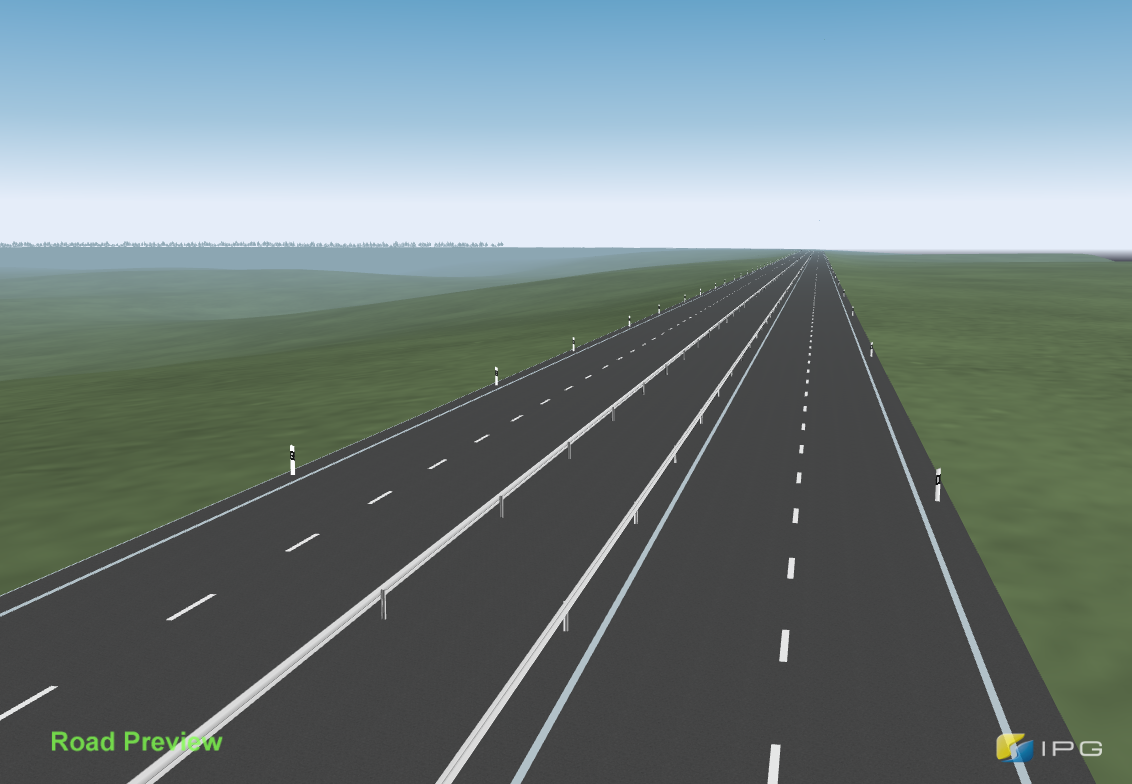
\includegraphics[scale=0.4]{cm_road_bild.png}
\caption{Konfiguration der simulierten Straße \cite{ipg2018carmaker}}
\label{fig_cm_road_bild}
\end{figure}

Auf beiden Strecken wird autonomer, stochastisch verteilter Verkehr erzeugt, was CarMaker mit einer gesonderten Funktion unterstützt. Der Verkehr wird in einer niedrigen Dichte (10\%) und einem 80\%-igen Anteil Autos erzeugt, andere Fahrzeuge sind Motorräder, Lastkraftwagen und Busse. In CarMaker ist eine Vielzahl an unterschiedlichen Fahrzeugen verfügbar, was wichtig ist um möglichst viele unterschiedliche Szenarien zu generieren. Mit dieser Konfiguration werden auf der 10.000m-Strecke 131 Fahrzeuge und auf der 6.000m-Strecke 89 Fahrzeuge generiert.

\begin{figure}[h]
\centering
\begin{tabular}{c}
\subfloat[Strecke 1]{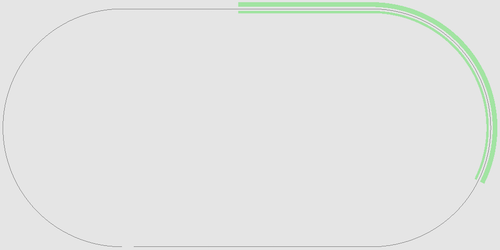
\includegraphics[scale=0.8]{cm_road_1.png}} \\
\subfloat[Strecke 2]{
\includegraphics[scale=0.8]{cm_road_2.png}}
\end{tabular}
\caption{Schema der simulierten Strecken 1 und 2 \cite{ipg2018carmaker}}
\label{fig_cm_road_strecke}
\end{figure}

Die Simulation und Generierung von Bild- und Signaldaten wird mit dem \textit{CarMaker - Test Manager} durchgeführt. Mit diesem Modul lassen sich Fahrten mit unterschiedlichen Konfigurationen simulieren. In dieser Arbeit werden die Variablen \textit{Geschwindigkeit}, \textit{Mindestabstand zu vorausfahrendem Fahrzeug}, \textit{Minimale Geschwindigkeitsdifferenz beim Überholen} und \textit{Aggressivität beim Überholen} auf beiden oben beschriebenen Strecken variiert. Die Werte der Variablen, die simuliert werden, sind in Tabelle \ref{tab_tm_variablen} aufgelistet und sind aus der Sicht des Ego-Fahrzeugs.

\begin{table}[h]
\small
\centering
\def\arraystretch{1.4}
\begin{tabular}{p{8cm} p{0.7cm} p{0.7cm} p{0.7cm} p{0.7cm} p{0.7cm}}
\textbf{Variable} & \textbf{Werte} & & & & \\
\hline
Geschwindigkeit in [km/h] & 100 & 120 & 140 & 160 & 180 \\
Mindestabstand zu vorausfahrendem Fahrzeug in [s] & 1,0 & 1,5 & 2,0 & & \\
Minimale Geschwindigkeitsdifferenz beim Überholen in [km/h] & 5 & 15 & 25 & & \\
Aggressivität beim Überholen & 0,2 & 0,6 & 1,0 & & \\
\hline
\end{tabular}
\caption{Variablen und Werte die in der Simulation verwendet werden}
\label{tab_tm_variablen}
\end{table}

Die ersten drei Variablen sind selbsterklärend und werden hier nicht weiter erläutert. Die Variable \textit{Aggressivität beim Überholen} (in CarMaker \textit{Overtaking Rate} ist eine Zahl zwischen 0 und 1. Dabei markiert die 0 ein Fahrstil, bei dem sich der Fahrer sehr risikoavers beim Überholen verhält, i.e. Überholen nur in sehr sicheren Situationen. Je größer die Zahl wird, desto aggressiver wird der Überholvorgang und dementsprechend sinkt die Risikoaversion beim Überholen und der Fahrer überholt auch bei kritischen oder schlecht einsehbaren Situationen.

Mit diesen vier Variablen mit jeweils drei bzw. fünf Werten ergeben sich 135 verschiedene Kombinationsmöglichkeiten. Somit werden auf beiden Strecken in Summe 270 Fahrten mit 2.160 km simuliert. Signal- und Bilddaten werden mit einer Frequenz von 5 Hz aufgezeichnet, was in 326.108 aufgezeichneten Szenen (Bilder und Signaldaten) resultiert. Diese Szenen werden im folgenden Abschnitt \ref{umsetzung_daten_synth_labeling} gelabelt.


% ===========================
\subsection{Daten Labeling}
\label{umsetzung_daten_synth_labeling}
% ===========================

Für das Labeln der Szenarien wird jede Szene auf Basis der Definition aus Abschnitt \ref{umsetzung_definition} mithilfe der Signaldaten klassifiziert. Die logischen Bedingungen für jedes Szenario sind dafür in Tabelle \ref{tab_szenarien_labeling} aufgelistet. Auf Basis der CarMaker-Variablen aus Tabelle \ref{tab_tm_variablen} werden folgende zusätzliche Variablen definiert, um nachfolgende Bedingungen übersichtlicher darzustellen. Dabei beschreibt $v2$ jeweils das Fahrzeug, auf Basis dessen das jeweilige Szenario klassifiziert wird.

\begin{equation*}
\begin{split}
ego_v = \text{Car.v} \qquad \text{[m/s]} \\
ego_{sRoad} = \text{Car.Road.sRoad} \qquad \text{[m]} \\
ego_{laneID} = \text{Car.Road.Lane.Act.LanId} \qquad \text{[1, 2]} \\
v2_{dv} = \text{Sensor.Object.OB01.TX.NearPnt.dv\_p} \qquad \text{[m/s]} \\
v2_{ds} = \text{Sensor.Object.OB01.TX.NearPnt.dv\_p} \qquad \text{[m]} \\
v2_{sRoad} = \text{Traffic.TX.sRoad} \qquad \text{[m]} \\
v2_{laneID} = \text{Traffic.TX.Lane.Act.LaneId} \qquad \text{[1, 2]} \\
\end{split}
\end{equation*}

\small
\begin{longtable}[c]{p{3cm} p{8.5cm}}
\textbf{Szenario} & \textbf{Bedingungen} \\
\hline
\endhead

\textbf{Free cruising} & $ego_v > 17$ \newline $s_0 < v2_{ds}$ \\
\hline
\textbf{Approaching} & $s_2 < v2_{ds} < s_0$ \newline $ego_{sRoad} < v2_{sRoad}$ \newline $ego_{laneID} == v2_{laneID}$ \newline $ego_v < \text{ Durchschnitt von } ego_v \text{ der letzten 3 Sekunden} $ \\
\hline
\textbf{Following} & $v2_{dv} < ego_v * 0,05$ \newline $s_3 < s_1$ \newline $ego_{sRoad} < v2_{sRoad}$ \newline $ego_{laneID} == v2_{laneID}$ \\
\hline
\textbf{Catching up} & $v2_{dv} < 0$ \newline $0 <= v2_{ds} < s_0$ \newline $ego_{sRoad} <= v2_{sRoad}$ \newline $ego_{laneID} == v2_{laneID} - 1$ \\
\hline
\textbf{Overtaking} & $0 <= v2_{ds} < s_0$ \newline $v2_{sRoad} < ego_{sRoad}$ \newline $ego_{laneID} == v2_{laneID} - 1$ \\
\hline
\textbf{Lane change left} & $ego_{laneID}^{before} == ego_{laneID}^{after} + 1$ \newline Als Spurwechsel wird ein Intervall von 4 Sekunden betrachtet in dessen Mitte die Variable ihren Wert wechseln muss\\
\hline
\textbf{Lane change right} & $ego_{laneID}^{before} == ego_{laneID}^{after} - 1$ \newline Als Spurwechsel wird ein Intervall von 4 Sekunden betrachtet in dessen Mitte die Variable ihren Wert wechseln muss \\

\hline
\caption{Bedingungen der Szenarien \textit{free cruising}, \textit{approaching}, \textit{following}, \textit{catching up}, \textit{overtaking}, \textit{lane change left} und \textit{lane change right}}
\label{tab_szenarien_labeling}
\end{longtable}
\normalsize

Im Anschluss an die Klassifizierung einzelner Zeitpunkte werden diese zu Szenarien zusammengefasst, wenn mindestens 15 Zeitpunkte (3 Sekunden) in Folge mit dem gleichen Label klassifiziert wurden. Drei Sekunden wird den folgenden zwei Gründen als Länge für Szenarien in dieser Arbeit gewählt. Erstens orientiert sich diese Zeitspanne an den vorherigen Arbeiten zur Szenarienerkennung. Zweitens haben die zwei Szenarien \textit{lane change left} und \textit{lane change right} jeweils eine natürliche Länge von 3-4 Sekunden. Alle anderen Szenarien können länger sein, lassen sich aber in Blöcke von jeweils 3 Sekunden einteilen. Insgesamt werden 326.108 Zeitpunkte und 23.972 Szenarien klassifiziert. Die Anzahl der simulierten Szenarien nach Klasse ist in der Tabelle \ref{tab_verteilung_szenarien} dargestellt.

\begin{table}[h]
\small
\centering
\def\arraystretch{1.4}
\begin{tabular}{l c}

\textbf{Szenario} & \textbf{Anzahl} \\
\hline
Free cruising & 2.545 \\
Approaching & 3.512 \\
Following & 3.601 \\
Catching up & 5.563 \\
Overtaking & 5.149 \\
Lane change left & 957 \\
Lane change right & 975 \\
Unknown & 1.670 \\
\hline
Summe & 23.972 \\
\hline

\end{tabular}
\caption{Anzahl der simulierten Szenarien nach Klasse}
\label{tab_verteilung_szenarien}
\end{table}

Es sind auch einige Szenarien als \textit{unknown} klassifiziert, da zwischen den definierten Szenarien andere Situationen auftreten können oder nicht die Mindestanzahl der konsekutiven Szenen erreicht wird. Zu manchen Zeitpunkten werden mehr als eine einzelne Szene klassifiziert. Beispielsweise kann sich das Ego-Fahrzeug gleichzeitig in der Szene \textit{catching up} und \textit{overtaking} befinden, wenn es auf der linken Fahrspur fährt und sich in vertikalem Abstand ein anderes Fahrzeug jeweils vor und hinter dem Ego-Fahrzeug befindet. Abbildung \ref{fig_beispiel_szenario_lcl} zeigt ein Beispiel des Szenarios \textit{lane change left} mit allen zugehörigen 15 Bildern.

\begin{figure}[h]
\centering
\begin{tabular}{c c c c c}
\subfloat[]{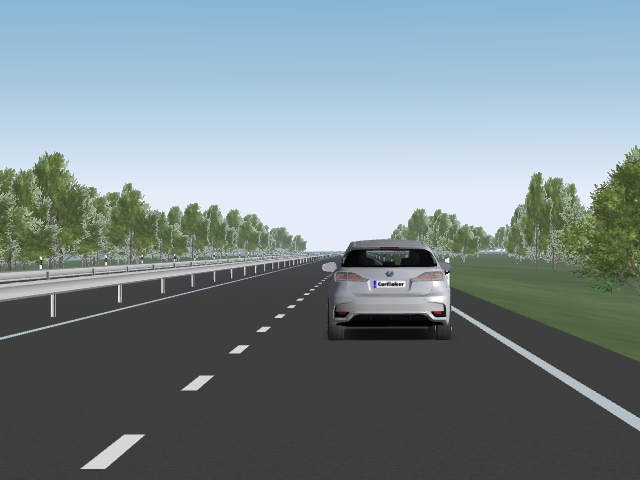
\includegraphics[scale=0.1]{lcl_sim/lcl0.jpg}} &
\subfloat[]{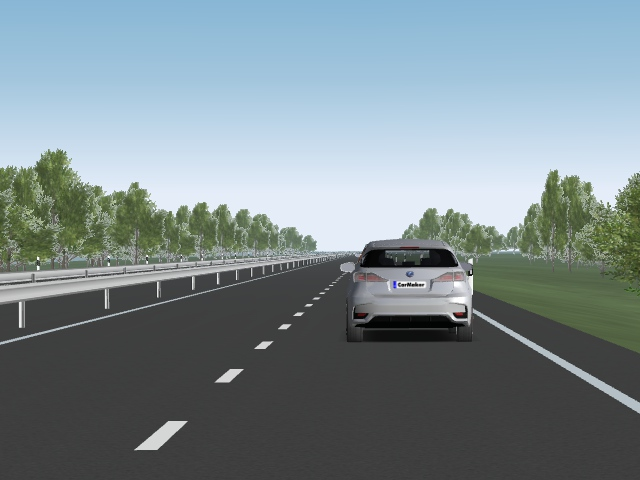
\includegraphics[scale=0.1]{lcl_sim/lcl1.jpg}} &
\subfloat[]{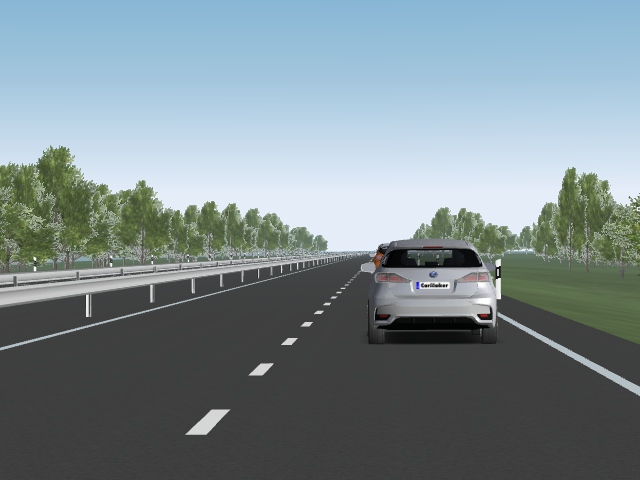
\includegraphics[scale=0.1]{lcl_sim/lcl2.jpg}} &
\subfloat[]{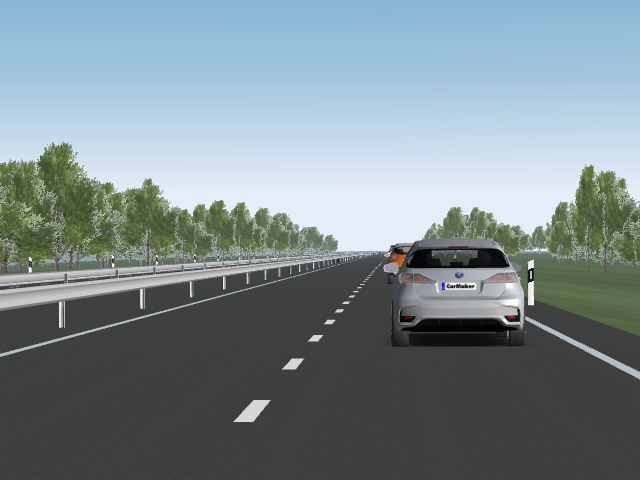
\includegraphics[scale=0.1]{lcl_sim/lcl3.jpg}} &
\subfloat[]{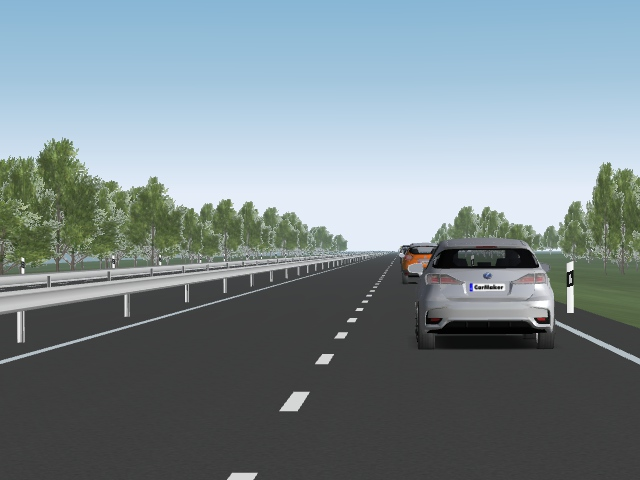
\includegraphics[scale=0.1]{lcl_sim/lcl4.jpg}} \\
\subfloat[]{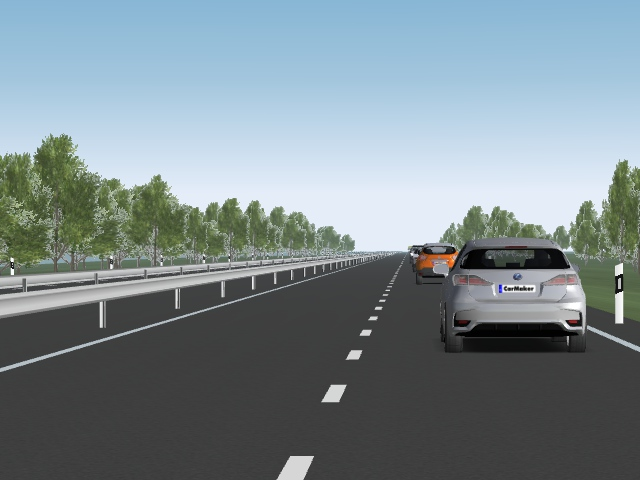
\includegraphics[scale=0.1]{lcl_sim/lcl5.jpg}} &
\subfloat[]{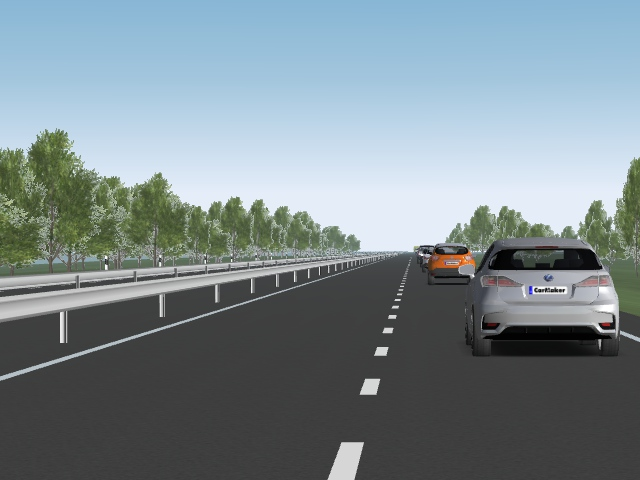
\includegraphics[scale=0.1]{lcl_sim/lcl6.jpg}} &
\subfloat[]{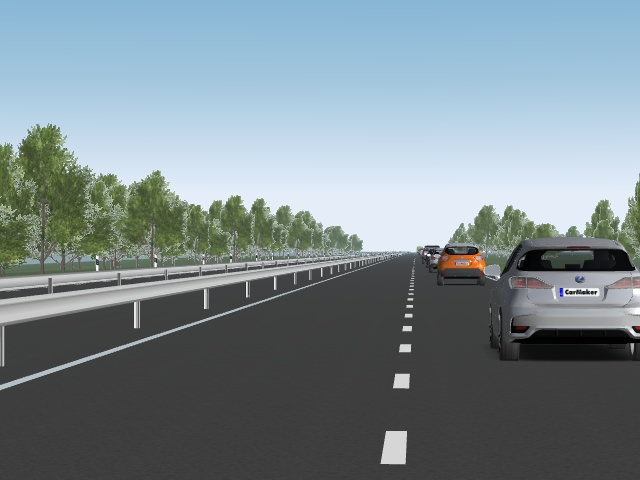
\includegraphics[scale=0.1]{lcl_sim/lcl7.jpg}} &
\subfloat[]{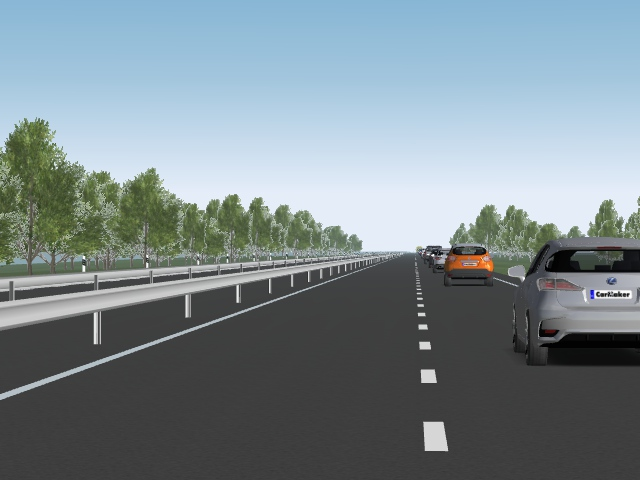
\includegraphics[scale=0.1]{lcl_sim/lcl8.jpg}} &
\subfloat[]{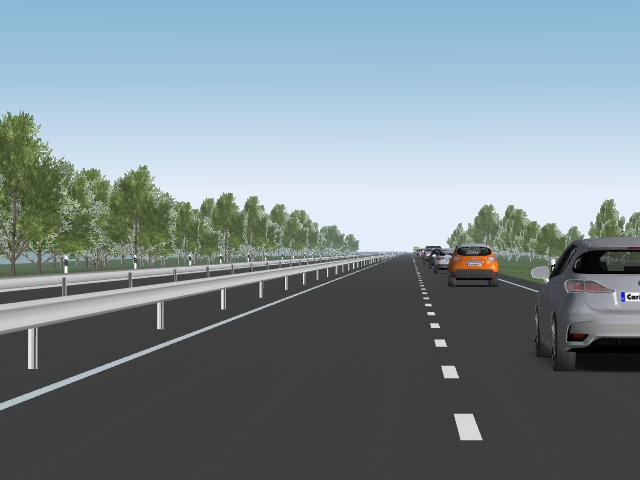
\includegraphics[scale=0.1]{lcl_sim/lcl9.jpg}} \\
\subfloat[]{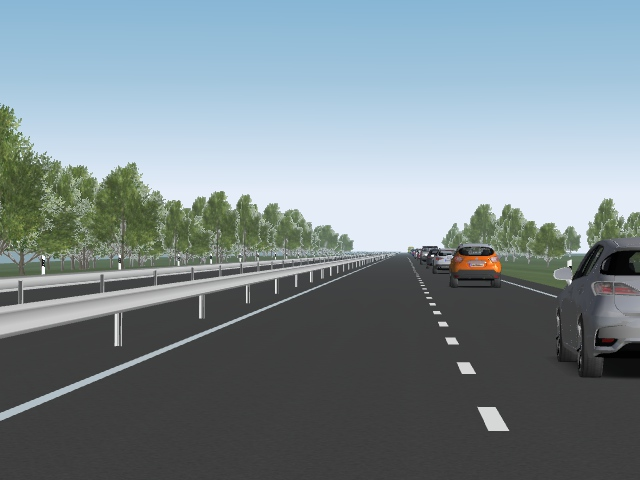
\includegraphics[scale=0.1]{lcl_sim/lcl10.jpg}} &
\subfloat[]{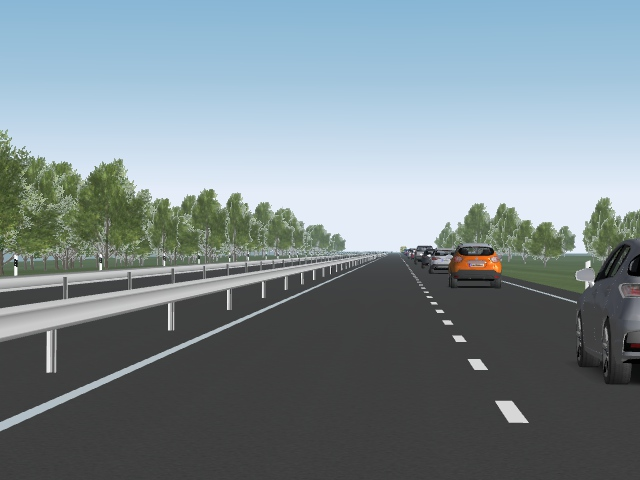
\includegraphics[scale=0.1]{lcl_sim/lcl11.jpg}} &
\subfloat[]{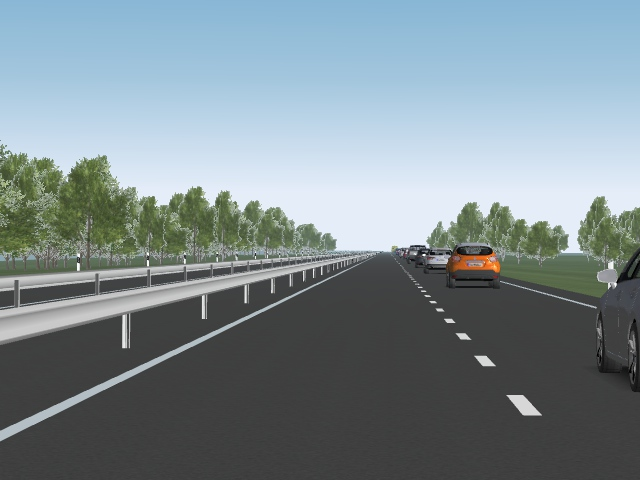
\includegraphics[scale=0.1]{lcl_sim/lcl12.jpg}} &
\subfloat[]{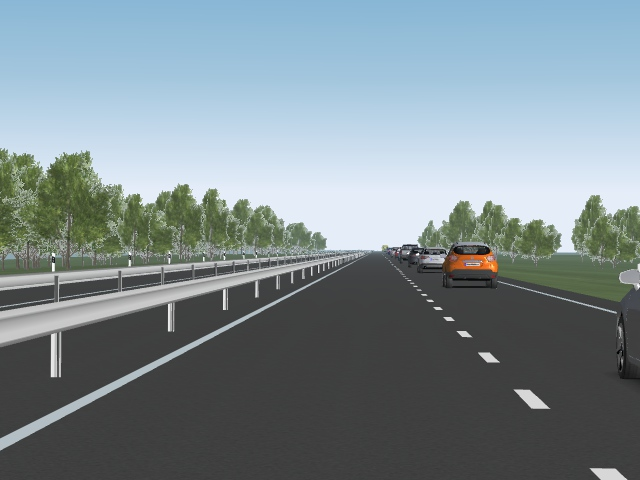
\includegraphics[scale=0.1]{lcl_sim/lcl13.jpg}} &
\subfloat[]{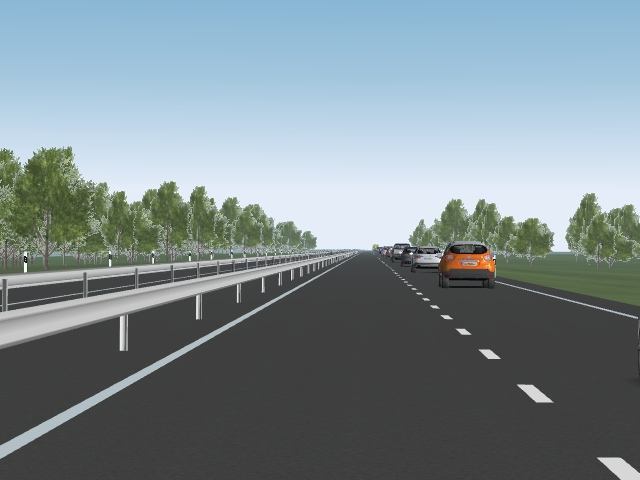
\includegraphics[scale=0.1]{lcl_sim/lcl14.jpg}} \\
\end{tabular}
\caption{Beispiel eines simulierten Szenarios der Klasse \textit{lane change left} \cite{ipg2018carmaker}}
\label{fig_beispiel_szenario_lcl}
\end{figure}


% ===========================
\section{Generierung realer Trainings- und Testdaten}
\label{umsetzung_daten_real}
% ===========================

Für den Proof-of-Concept dieser Arbeit, die Erkennung von realen Fahrszenarien, werden neben den synthetischen Trainingsdaten auch reale Daten für das Training und die anschließenden Tests benötigt. Dafür werden im ersten Schritt bestehen Datensätze nach ihrer Nutzbarkeit untersucht.

Die bekanntesten Datensätze sind KITTI \cite{geiger2013vision}, BDD100K \cite{yu2018bdd100k}, Cityscapes \cite{cordts2016cityscapes} und Oxford RobotCar \cite{maddern20171}. Der Cityscapes und Oxford RobotCar Datensatz umfasst lediglich Bilder von Szenen in Städten und ist daher nicht nutzbar für diese Arbeit. Die Datensätze KITTI und BDD100K umfassen auch Videos von Autobahnfahrten, allerdings liegt der Fokus auf Objekterkennung in einzelnen Bildern oder semantischer Segmentation. Und es gibt jeweils nur sehr begrenzt Videos, die auf einer 2-spurigen Autobahn aufgenommen wurden. Daher können diese Datensätze in dieser Arbeit nicht verwendet werden.

Als Alternative werden die Aufnahmen von zwei Fahrten auf der Autobahn und Bundesstraße verwendet. Die Strecken sind in der Abbildung \ref{fig_strecken_real} abgebildet. 

\begin{figure}[h]
\centering
\begin{tabular}{c c}
\subfloat[Route 1: Mannheim - Rostock]{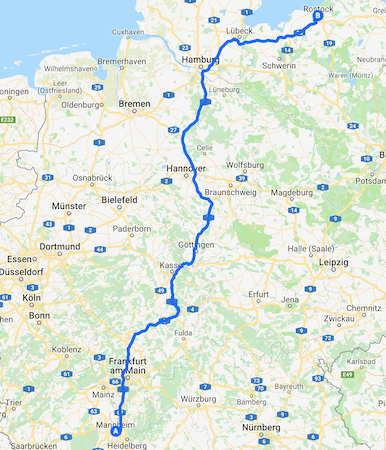
\includegraphics[scale=0.7]{route_1.png}} &
\subfloat[Route 2: Karlsruhe - Kandel]{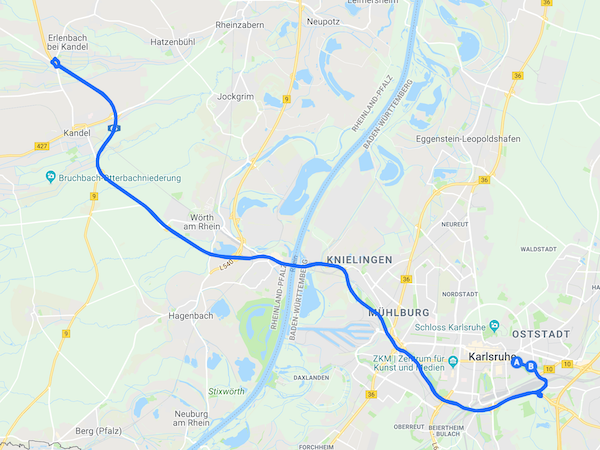
\includegraphics[scale=0.7]{route_2.png}} \\
\end{tabular}
\caption{Routen für die Aufnahme der realen Bilddaten \cite{google2018route1, google2018route2}}
\label{fig_strecken_real}
\end{figure}

Die Aufnahme der Route 1 umfasst über sechs Stunden Videomaterial mit über einer Stunde Fahrt auf einer 2-spurigen Autobahn \cite{youtube2018video}. Davon werden manuell zwischen 50 und 180 Szenarien aus jeder Klasse gelabelt. Da von den Szenarien \textit{lane change left} und \textit{lane change right} jeweils nur 50 Szenarien vorhanden sind, wird vom Autor eine Fahrt auf Route 2 mit einigen Spurwechseln aufgenommen. Das Ergebnis sind jeweils 17 weitere Szenarien in den Klassen \textit{lane change left} und \textit{lane change right}.Abbildung \ref{fig_beispiel_szenario_lcr_real} zeigt ein Beispiel des realen Szenarios \textit{lane change right} mit allen zugehörigen 15 Bildern.

\begin{figure}[h]
\centering
\begin{tabular}{c c c c c}
\subfloat[]{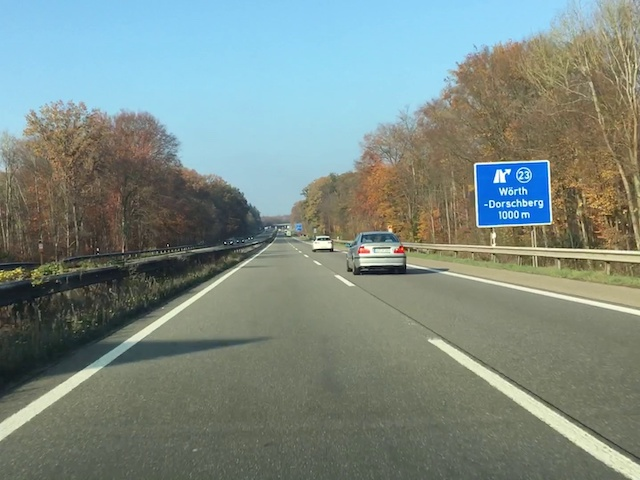
\includegraphics[scale=0.1]{lcr_real/frame0.jpg}} &
\subfloat[]{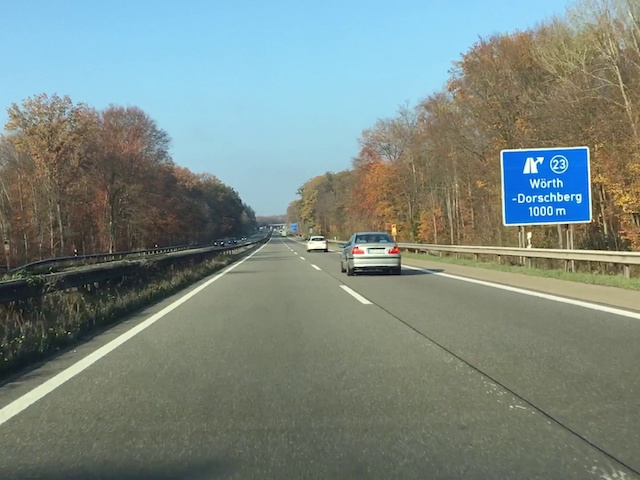
\includegraphics[scale=0.1]{lcr_real/frame1.jpg}} &
\subfloat[]{\includegraphics[scale=0.1]{lcr_real/frame2.jpg}} &
\subfloat[]{\includegraphics[scale=0.1]{lcr_real/frame3.jpg}} &
\subfloat[]{\includegraphics[scale=0.1]{lcr_real/frame4.jpg}} \\
\subfloat[]{\includegraphics[scale=0.1]{lcr_real/frame5.jpg}} &
\subfloat[]{\includegraphics[scale=0.1]{lcr_real/frame6.jpg}} &
\subfloat[]{\includegraphics[scale=0.1]{lcr_real/frame7.jpg}} &
\subfloat[]{\includegraphics[scale=0.1]{lcr_real/frame8.jpg}} &
\subfloat[]{\includegraphics[scale=0.1]{lcr_real/frame9.jpg}} \\
\subfloat[]{\includegraphics[scale=0.1]{lcr_real/frame10.jpg}} &
\subfloat[]{\includegraphics[scale=0.1]{lcr_real/frame11.jpg}} &
\subfloat[]{\includegraphics[scale=0.1]{lcr_real/frame12.jpg}} &
\subfloat[]{\includegraphics[scale=0.1]{lcr_real/frame13.jpg}} &
\subfloat[]{\includegraphics[scale=0.1]{lcr_real/frame14.jpg}} \\
\end{tabular}
\caption{Beispiel eines realen Szenarios der Klasse \textit{lane change right}}
\label{fig_beispiel_szenario_lcr_real}
\end{figure}


% ===========================
\section{Training}
\label{umsetzung_training}
% ===========================

In diesem Abschnitt wird zu Beginn das Format und der Import der Trainings- und Testdaten in das \ac{KNN} erklärt. Danach werden verschiedene Architekturen von \acp{KNN}, die in dieser Arbeit zum Einsatz kommen, vorgestellt und schließlich werden die durchgeführten Experimente mit diesen Architekturen erläutert. Die Vorbereitung der Daten und das Training wird mit Python und der Deep-Learning-Bibliothek Keras \cite{chollet2015keras} implementiert.


% ===========================
\subsection{Inputdaten}
\label{umsetzung_training_input}
% ===========================

Die Generierung der synthetischen und realen Trainings- und Testdaten wurde bereits in den vorherigen Abschnitten beschrieben. In diesem Abschnitt soll kurz darauf eingegangen werden wie diese Daten in das jeweilige \ac{KNN} eingespeist werden.

In dieser Arbeit werden \acp{CNN} für die Erkennung einzelner Bilder und Kombinationen aus \acp{CNN} und \ac{LSTM} für die Klassifizierung von Videos eingesetzt. Daher müssen sowohl einzelne Bilder, als auch Bildsequenzen in das jeweilige \ac{KNN} importiert werden. Da es sich um große Datenmengen von über 50GB handelt, müssen die Daten mit einem Datenstrom eingespeist werden, da nicht alle Daten zu Beginn in den Arbeitsspeicher geladen werden können.

Die Deep-Learning-Bibliothek Keras hat bereits sogenannte \textit{DataGenerators} für der Import von einzelnen Bildern und für sequenzielle Daten mit zwei Dimensionen (e.g. CSV-Dateien). Es gibt allerdings keine bereits nutzbare Lösung für den Import von sequentiellen Bildern, was 4-dimensionalen Daten entspricht (Anzahl Bilder, Höhe, Breite, Farbkanal). Aus diesem Grund wird die Lösung von Amidi \ref{amidi2017datagenerator} adaptiert um höher-dimensionale Datensets importieren zu können.

Von den generierten synthetischen und realen Szenarien werden \textit{free cruising}, \textit{following}, \textit{catching up}, \textit{lane change left} und \textit{lane change right} für das Training ausgewählt. Das Szenario \textit{approaching} wurde für den Proof-of-Concept in dieser Arbeit bewusst entfernt, weil es oft Überscheidungen mit dem Szenario \textit{following} gibt. Diese Überschneidungen und Ähnlichkeiten zwischen Szenarien und ihren Einfluss auf das Training eines Klassifikators können in weiteren Arbeiten untersucht werden. Das Szenario \textit{overtaking} wurde entfernt, weil es mit der konfigurierten Frontkamera allein nicht erfasst werden kann. In folgenden Arbeiten kann dieses Szenario mithilfe weiterer Kameraperspektiven zusätzlich berücksichtigt werden.

Um das Ergebnis nicht zu verzerren, sollten für das Training mit neuronalen Netzen in jeder Klasse jeweils die gleiche Anzahl an Trainings- und Testdaten vorhanden sein. Aus diesem Grund werden für das Training aus jeder Klasse nur die Anzahl der Szenarien verwendet, die mindestens in jeder Klasse verfügbar sind. Damit dieser Ansatz auch in der Praxis verwendet werden kann wird außerdem darauf geachtet, dass 95\% synthetische Daten und 5\% reale Daten für das Training verwendet werden. Mit dieser Verteilung bleibt der manuelle Aufwand für das Labeln der Trainingsdaten überschaubar. Die daraus resultierende Aufteilung von synthetischen und realen Szenarien auf Trainings-, Validierungs- und Testdaten ist in Tabelle \ref{tab_daten_aufteilung} aufgeschlüsselt. Beim Training mit einzelnen Bildern wird die gleiche Verteilung angewendet und da jedes Szenario aus 15 Bilder besteht, können die Zahlen aus Tabelle \ref{tab_daten_aufteilung} einfach mit 15 multipliziert werden.

\begin{table}[h]
\small
\centering
\def\arraystretch{1.4}
\begin{tabular}{l | c c c c c c | c}

& \multicolumn{3}{c}{\textbf{Synthetische Daten}} & \multicolumn{3}{c|}{\textbf{\textbf{Reale Daten}}} & \\
& Training & Validierung & Test & Training & Validierung & Test & \\
Szenario & 85\% & 10\% & 5\% & 65\% & 10\% & 25\% & Summe \\
\hline
free cruising & 807 & 95 & 48 & 43 & 7 & 17 & 1.017 \\
following & 807 & 95 & 48 & 43 & 7 & 17 & 1.017 \\
catching up & 807 & 95 & 48 & 43 & 7 & 17 & 1.017 \\
lane change left & 807 & 95 & 48 & 43 & 7 & 17 & 1.017 \\
lane change right & 807 & 95 & 48 & 43 & 7 & 17 & 1.017 \\
\hline
\textbf{Summe} & \textbf{4.035} & \textbf{475} & \textbf{240} & \textbf{215} & \textbf{35} & \textbf{85} & 5.085 \\
\hline

\end{tabular}
\caption{Aufteilung von synthetischen und realen Szenarios auf Trainings-, Validierungs- und Testdaten}
\label{tab_daten_aufteilung}
\end{table}

Die Bilddaten werden für das Training außerdem in die Form 299 x 299 x 3 Pixel transformiert. Diese Bildgröße ist ein Kompromiss zwischen Detailgrad und Trainingszeit und wird in Keras, neben der Auflösung 244 x 244 x 3 Pixel, für \acp{CNN} als Standardkonfiguration vorgeschlagen \cite{chollet2015keras}.

% ===========================
\subsection{Architektur der künstlichen neuronalen Netze}
\label{umsetzung_training_architektur}
% ===========================

In diesem Abschnitt werden verschiedene Architekturen von tiefen \acp{KNN} vorgestellt, die im nächsten Abschnitt \ref{umsetzung_training_experimente} für die Experimente in dieser Arbeit verwendet werden. Wie in Abschnitt \ref{grundlagen_nn_video} erläutert, gibt es verschiedenen Ansätze um Bildsequenzen mit \acp{KNN} zu klassifizieren. In dieser Arbeit werden zwei unterschiedliche Ansätze umgesetzt und miteinander verglichen. Im ersten Ansatz werden die Bilder in den Sequenzen einzeln klassifiziert. Anschließend wird den Sequenzen die Klasse zugeordnet, mit der die meisten Bilder in der Sequenz klassifiziert wurden. Für den zweiten Ansatz wird eine Kombination aus Bild- und Sequenzerkennung verwendet um die Bildsequenzen als ganzes zu klassifizieren. Die Architekturken für den jeweiligen Ansatz werden in den folgenden Absätzen vorgestellt.

Beim ersten Ansatz handelt es sich um die Klassifizierung von einzelnen Bildern, wofür \acp{CNN} verwendet werden. Das Training mit \acp{CNN} hat in den vergangenen Jahre große Fortschritte gemacht durch die Verfügbarkeit von großen Datenmengen, steigender Rechenleistung und die Wiederverwendung von bereits vortrainierten \acp{CNN}. Diese Verwendung von bereits trainierten Netzen nennt sich Transferlernen (engl. transfer learning) \cite{oquab2014transfer}. Die Idee von einem \ac{CNN} ist es in den frühen Schichten sehr grundlegende Merkmale (engl. low-level features) und in späteren Schichten abstraktere Merkmale (engl. high-level features) zu extrahieren. Schließlich wird Bilder auf Basis dieser abstrakten Merkmale mithilfe von einer oder mehreren Fully-Connected-Schichten klassifiziert. Diese Funktionsweise macht man sich beim Transferlernen zunutze und verwendet ein \ac{CNN} das bereits auf vielen Millionen Bildern trainiert wurde. Dieses \ac{CNN} hat bereits gelernt unterschiedliche Merkmale aus Bildern zu extrahieren. Um ein ein solches neuronales Netz für die eigene Arbeit verwenden zu können, muss man lediglich die letzten Fully-Connected-Schichten ersetzen und mit den eigenen Bilddaten und entsprechenden Klassen trainieren \cite{oquab2014transfer}. Mit diesem Verfahren kann viel Zeit und Rechenleistung gespart werden, weil die grundlegende Merkmalsextraktion nicht grundlegend neu gelernt werden muss. 

Das Transferlernen wird auch in dieser Arbeit verwendet. Dazu wurden verschiedene \ac{CNN}-Architekturen verglichen und schließlich zwei unterschiedliche für diese Arbeit ausgewählt. Eine Übersicht der bekanntesten vortrainierten \acp{CNN} ist in Abbildung \ref{fig_comparison_cnns} dargestellt. In dieser Darstellung werden die neuronalen Netze anhand ihrer erreichen Genauigkeit (engl. accuracy) und der benötigten Operationen bzw. ihrer Parameter bei der Berechnung einer Klassifizierung eingeordnet \cite{canziani2016analysis}.

\begin{figure}[h]
\centering
\includegraphics[scale=0.35]{comparison_cnns.png}
\caption{Vergleich von vortrainierten \aclp{CNN}, entnommen aus \cite{canziani2016analysis}}
\label{fig_comparison_cnns}
\end{figure}

Für die Architekturen in dieser Arbeit werden die \acp{CNN} Inception-V3 \cite{szegedy2016inception} und VGG-16 \cite{simonyan2014vgg} als Basis verwendet, weil beide in vergangene Wettbewerben und anderen Arbeiten sehr gute Ergebnisse erzielen konnten.

Das VGG-16 Netz 
138,357,544

ImageNet ist ein Datensatz mit 14.197.122 Bildern und 21.841 sogenannten Synonymmengen (engl. synonym sets) \cite{deng2009imagenet}. In Synonymmengen sind Wörter der gleichen Bedeutung zusammengefasst. Dabei sind alle Wörter auch hierarchisch nach dem WordNet-Projekt eingeordnet.

Im Gegensatz zu einfach gestapelten Convolution- und Pooling-Schichten wie beispielsweise dem VGG-16 Netz, orientiert sich das Inception-V3 Netz an zusätzlichen Prinzipen, um die Genauigkeit zu verbessern und die Rechenleistung zu senken. Zusätzlich werden Convolution-Operationen nicht nur gestapelt, sondern auch parallel zu anderen Convolution-Operationen berechnet, was zu einer besseren Leistung des Netzes führt \cite{szegedy2016inception}. 

Es wird argumentiert, dass ein Filter mit der Dimension 5x5 durch zwei aufeinanderfolgende Filter der Dimension 3x3 ersetzt werden kann, was die Rechenleistung deutlich reduziert \cite{szegedy2016inception}. Diese Funktionalität wird in einem sogenannten Inception-Modul umgesetzt, was in Abbildung \ref{fig_inc_fig} unter (a) zu sehen ist. Ein weiteres Prinzip ist, dass ein nxn-Filter mit einen 1xn-Filter gefolgt von einem nx1 Filter ersetzt werden kann, bei gleichbleibender Leistung und 33\% weniger Rechenaufwand. Dieses Prinzip ist in Abbildung \ref{fig_inc_fig} unter (b) dargestellt. Für das dritte Prinzip wird argumentiert, dass bei einer starken Dimensionsreduzierung durch Pooling-Schichten viel Information aus dem Bild verloren gehen kann. Um dies zu verhindern, werden statt einer Pooling-Schicht mehrere parallele Convolution-Operationen ausgeführt. Dieses Prinzip wird mit dem Inception-Modul aus Abbildung \ref{fig_inc_fig} unter (c) umgesetzt.

\begin{figure}[h]
\centering
\begin{tabular}{c c}
\subfloat[Inception-Modul in dem ein 5x5-Filter mit zwei 3x3-Filter ersetzt wird]{\includegraphics[scale=0.35]{inc_fig_5.pdf}} &
\subfloat[Inception-Modul in dem ein 7x7-Filter mit einen 1x7-Filter gefolgt von einem 7x1 Filter ersetzt wird]{\includegraphics[scale=0.35]{inc_fig_6.pdf}} \\
\subfloat[Inception-Modul in statt einer Pooling-Schicht mehrere parallele Convolution-Operationen ausgeführt werden]{\includegraphics[scale=0.35]{inc_fig_7.pdf}} &
\end{tabular}
\caption{Inception-Module aus der Inception-V3 Architektur \cite{szegedy2016inception}}
\label{fig_inc_fig}
\end{figure}

Die Architektur des gesamten Netzes ist in Abbildung \ref{fig_inception_v3} dargestellt. In dieser Arbeit wird ein Inception-V3 Netz verwendet, das mit dem Datenset ImageNet \cite{deng2009imagenet} trainiert wurde.

\begin{figure}[h]
\centering
\includegraphics[scale=0.45]{inception_v3.png}
\caption{Architektur des Inception-V3 Netzes, entnommen aus \cite{google2018inceptionv3}}
\label{fig_inception_v3}
\end{figure}



% ===========================
\subsection{Experimente}
\label{umsetzung_training_experimente}
% ===========================

 Stet clita kasd gubergren, no sea takimata sanctus est Lorem ipsum dolor sit amet. Lorem ipsum dolor sit amet, consetetur sadipscing elitr, At accusam aliquyam diam diam dolore dolores duo eirmod eos erat, et nonumy sed tempor et et invidunt justo labore Stet clita ea et gubergren, kasd magna no rebum. sanctus sea sed takimata ut vero voluptua. est Lorem ipsum dolor sit amet. Lorem ipsum dolor sit amet, consetetur
 
 Dropout - \cite{hinton2012improving}
 \cite{srivastava2014dropout}

 
 





% ===========================
\chapter{Ergebnis}
\label{ergebnis}
% ===========================

In diesem Kapitel werden die Ergebnisse der trainierten \acp{KNN} aus Abschnitt \ref{umsetzung_training_architektur} mit den Parametern aus Abschnitt \ref{umsetzung_training_experimente} vorgestellt. Jede Architektur wird mit einer Maximalanzahl von 100 Epochen trainiert. Aufgrund der Regularisierungsmethode Early Stopping wird diese Anzahl jedoch nie erreicht. Das Training bricht jeweils ab, wenn sich die Klassifizierungsgenauigkeit der Validierungsdaten innerhalb von 20 Epochen nicht um mindestens 0,01 verbessert. Nach Abbruch werden jeweils die Gewichte der Epoche mit der höchsten Genauigkeit wiederhergestellt. 

In Abschnitt \ref{ergebnis_parameter} wird die Genauigkeit der jeweiligen Netzarchitekturen bei der Klassifizierung der realen Testdaten und die Anzahl der trainierten Epochen hinsichtlich der unterschiedlichen Parameter aus Abschnitt \ref{umsetzung_training_experimente} verglichen. Danach wird in Abschnitt \ref{ergebnis_synth_vs_real} die Genauigkeit der Klassifizierung zwischen realen und synthetischen Testdaten untersucht. Im Anschluss werden in Abschnitt \ref{ergebnis_szenarien} die Unterschiede bei der Erkennung von verschiedenen Klassen erörtert.


% ===========================
\section{Variation der Parameter}
\label{ergebnis_parameter}
% ===========================

In diesem Abschnitt werden die Unterschiede der verschiedenen Architekturen aus Abschnitt \ref{umsetzung_training_architektur} noch einmal kurz aufgegriffen und dann die dazugehörigen Ergebnisse vorgestellt. Die Ergebnisse sind in Tabelle \ref{tab_ergebnis_real} zusammengefasst.

\begin{table}[h]
\small
\centering
\def\arraystretch{1.4}
\begin{tabular}{c p{3cm} c c}
\textbf{Architektur} & \textbf{Beschreibung} & \textbf{Genauigkeit} & \textbf{Epochen} \\
\hline
A & Inception-V3 & 0,73 & 4 \\
\hline
B & Inception-V3 \newline Dropout & 0,64 & 1 \\
\hline
C & Xception & 0,54 & 1 \\
\hline
D & Xception \newline Dropout & 0,48 & 9 \\
\hline 
E & Inception-V3 \newline LSTM & 0,36 & 80 \\
\hline
F & Inception-V3 \newline LSTM \newline Dropout & 0,95 & 12 \\
\hline
G & Xception \newline LSTM & 0,38 & 26 \\
\hline
H & Xception \newline LSTM \newline Dropout & 0,61 & 9 \\
\hline
\end{tabular}
\caption{Ergebnisse der verschiedenen Architekturen bei der Klassifizierung der realen Testdaten}
\label{tab_ergebnis_real}
\end{table}

% ===========================
\subsubsection{Prinzip der Klassifizierung}
% ===========================

Bei dem Prinzip der Klassifizierung wird in dieser Arbeit zwischen \acp{KNN} für die Erkennung von einzelnen Bildern und für die Erkennung von 3-Sekunden-Videos mit jeweils 15 Bildern unterschieden. Die detaillierten Architekturen sind in Abschnitt \ref{umsetzung_training_architektur} vorgestellt.

Insgesamt wird die höchste Genauigkeit bei der Klassifizierung der realen Testdaten von 0,95 mit der Architektur F für Videoerkennung erreicht. Dieses Ergebnis ist auch in Abbildung \ref{fig_cm_v3_lstm_d_real} in der Konfusionsmatrix (engl. confusion matrix) dargestellt. Die niedrigste Genauigkeit von 0,28 wird mit der Architektur H für Videoerkennung erreicht. Architekturen für die reine Bilderkennung erreichen Genauigkeiten zwischen 0,48 (Architektur D) und 0,73 (Architektur A). Damit erzielen diese Architekturen Ergebnisse mit weniger Varianz im Vergleich zu den Architekturen mit \ac{LSTM}-Schicht.

\begin{figure}[h]
\centering
{\includegraphics[scale=0.7]{cm_v3_lstm_d_real.png}}
\caption{Konfusionsmatrix der Klassifizierung von realen Testdaten mit der Architektur F (Inception-V3, \ac{LSTM}, Dropout)}
\label{fig_cm_v3_lstm_d_real}
\end{figure}

% ===========================
\subsubsection{\aclp{CNN}}
% ===========================

Der Vergleich zwischen den zwei \ac{CNN}-Architekturen Inception-V3 und Xception zeigt ein klares Bild. In drei von vier Fällen kann die Architektur mit der Inception-V3-Architektur als Basis bessere Ergebnisse erzielen. Die Differenz bei der Genauigkeit liegt dabei zwischen 0,16 und 0,67. Nur die Architektur G erzielt eine höhere Genauigkeit als Architektur E mit einem Unterschied von 0,02. Insgesamt überrascht dieser Unterschied, da die Xception-Architektur in anderen Arbeiten \cite{chollet2017xception} höhere Genauigkeiten bei der Klassifizierung von Bildern erreicht hat.

% ===========================
\subsubsection{Regularisierung mit Dropout}
% ===========================

Es ist auffällig, dass die Architekturen für Videoklassifizierung mit Dropout in der vorletzten Fully-Connected-Schicht deutlich bessere Ergebnisse erzielen können im Vergleich zu denselben Architekturen ohne Dropout. Im Gegensatz dazu erzielen die Architekturen für die Erkennung einzelner Bilder die bessere Genauigkeit ohne Regularisierung mit Dropout in der vorletzten Schicht.

In Abbildung \ref{fig_acc_v3_lstm} ist beispielhaft die Entwicklung der Genauigkeit der Trainings- und Testdaten während dem Training von den Architekturen E und F dargestellt. Es ist deutlich zu sehen, dass die Anzahl der Epochen bei Architekturen mit \ac{LSTM}-Schicht mit Dropout stark reduziert werden kann und die Genauigkeit weniger sprunghaft und schneller konvergiert.

\begin{figure}[h]
\centering
\begin{tabular}{cc}
\subfloat[Architektur E (Inception-V3, LSTM)]{\includegraphics[scale=0.4]{acc_v3_lstm_86.png}} &
\subfloat[Architektur F (Inception-V3, LSTM, Dropout)]{\includegraphics[scale=0.4]{acc_v3_lstm_dropout_23.png}}
\end{tabular}
\caption{Genauigkeit der Trainings- und Testdaten während dem Training von zwei verschiedenen Architekturen}
\label{fig_acc_v3_lstm}
\end{figure}

Eine mögliche Erklärung dafür könnte die Komplexität der Architekturen mit \ac{LSTM}-Schicht sein. Diese Architekturen haben mehr trainierbare Parameter und sind daher anfälliger für eine Überanpassung \cite{hinton2012improving}. Regularisierung mit Dropout kann die Komplexität reduzieren und führt zu höheren Genauigkeiten \cite{hinton2012improving}. Die Architekturen mit reinen \acp{CNN} sind weniger komplex und daher könnte Dropout keine oder eine negative Auswirkung auf das Ergebnis haben.

% ===========================
\subsubsection{Anzahl der Epochen}
% ===========================

Es lässt sich beobachten, dass die Architekturen für die Klassifizierung von Videos mit bis zu 86 Epochen deutlich mehr Trainingsschritte benötigen als die Architekturen für reine Bilderkennung. Eine mögliche Erklärung dafür ist, dass reine \acp{CNN} eine weniger komplexe Architektur und weniger Parameter haben als die Architekturen mit einer \ac{LSTM}-Schicht. Mehr Gewichte, die angepasst werden können, bedeutet eine höhere Komplexität und dementsprechend mehr benötigte Epochen.

Zu den Unterschieden der Epochenanzahl zwischen der Inception-V3- und der Xception-Architektur lässt sich in dieser Arbeit keine eindeutige Aussage treffen. Die benötige Epochenanzahl bei beiden Architekturen variiert sehr stark.

% ===========================
\section{Synthetische und reale Testdaten}
\label{ergebnis_synth_vs_real}
% ===========================

\begin{table}[h]
\small
\centering
\def\arraystretch{1.4}
\begin{tabular}{c p{3cm} c c}
\textbf{Architektur} & \textbf{Beschreibung} & \textbf{Genauigkeit} & \textbf{Genauigkeit} \\
 & & \textbf{Reale Testdaten} & \textbf{Synthetische Testdaten} \\
\hline
A & Inception-V3 & 0,73 & 0,96 \\
\hline
B & Inception-V3 \newline Dropout & 0,64 & 0,96 \\
\hline
C & Xception & 0,54 & 0,2 \\
\hline
D & Xception \newline Dropout & 0,48 & 0,36 \\
\hline 
E & Inception-V3 \newline LSTM & 0,36 & 0,94 \\
\hline
F & Inception-V3 \newline LSTM \newline Dropout & 0,95 & 0,99 \\
\hline
G & Xception \newline LSTM & 0,38 & 0,99 \\
\hline
H & Xception \newline LSTM \newline Dropout & 0,61 & 0,91 \\
\hline
\end{tabular}
\caption{Ergebnisse der Klassifizierung von synthetischen und realen Testdaten}
\label{tab_ergebnis_synth}
\end{table}

In diesem Abschnitt werden die Unterschiede der Genauigkeiten bei der Klassifizierung zwischen realen und synthetischen Testdaten untersucht. Die Ergebnisse sind in Tabelle \ref{tab_ergebnis_synth} zusammengefasst. Es ist nicht überraschend, dass die Genauigkeiten bei der Klassifizierung von synthetischen Testdaten überwiegend deutlich höher ist, weil die \acp{KNN} mit 95\% synthetischer und nur 5\% realer Daten trainiert wurden. Das bestätigt auch die Ergebnisse der vorangegangenen Arbeit, die in Abschnitt \ref{grundlagen_nn_synthetisch} diskutiert werden. 

Es ist auffällig, dass die Klassifizierung von einzelnen synthetischen Bildern mit der Xception Architektur niedriger ist als die Klassifizierung von realen Testbildern. Aktuell hat der Autor keine Erklärung hierfür. Dieses Ergebnis kann als Ausgangspunkt für weitere Arbeiten dienen.


% ===========================
\section{Genauigkeit der einzelnen Szenarien}
\label{ergebnis_szenarien}
% ===========================

Die Betrachtung von Klassifizierungsgenauigkeiten der einzelnen Klassen ergibt kein eindeutiges Bild. Bei verschiedenen Architekturen werden verschiedene Szenen teilweise besser oder schlechter erkannt. Hervorzuheben ist, dass es deutliche Unterschiede gibt, diese aber keinem erkennbaren Muster folgen. Eine Übersicht der Genauigkeit der Klassifizierung von realen Testdaten auf der Ebene von Szenarienklassen ist in Tabelle \ref{tab_ergebnis_szenarien} dargestellt.

\begin{table}[h]
\small
\centering
\def\arraystretch{1.4}
\begin{tabular}{c c c c c c}
\textbf{Architektur} & \textbf{Free} & \textbf{Following} & \textbf{Catching} & \textbf{Lane change} & \textbf{Lane change} \\
 & \textbf{cruising} & & \textbf{up} & \textbf{left} & \textbf{right} \\
\hline
A & 0,65 & 0,76 & 1,00 & 0,35 & 0,88 \\
B & 0,94 & 0,47 & 0,88 & 0,29 & 0,59 \\
C & 0,76 & 0,94 & 0,94 & 0,00 & 0,06 \\
D & 0,00 & 0,82 & 0,82 & 0,76 & 0,00 \\
E & 0,59 & 0,47 & 0,41 & 0,06 & 0,29 \\
F & 0,88 & 0,94 & 1,00 & 0,94 & 1,00 \\
G & 0,47 & 0,06 & 0,18 & 0,59 & 0,06 \\
H & 0,71 & 1,00 & 0,71 & 0,35 & 0,29 \\
\hline
\textbf{Durchschnitt} & 0,62 & 0,68 & 0,74 & 0,42 & 0,40 \\
\hline
\end{tabular}
\caption{Genauigkeit der Klassifizierung von realen Testdaten auf der Ebene von Szenarienklassen}
\label{tab_ergebnis_szenarien}
\end{table}

Um an dieser Stelle besser verstehen zu können auf welcher Basis die \acp{KNN} die Bilder beziehungsweise die Bildsequenzen erkennen, sollten in nachfolgenden Arbeiten weitere Untersuchungen dazu angestellt werden. So wäre es beispielsweise interessant, welche Teile der einzelnen Bilder stärker oder auch weniger stark bei der Klassifizierung berücksichtigt werden.














% ===========================
\chapter{Zusammenfassung}
\label{zusammenfassung}
% ===========================

In dieser Arbeit wurde ein Konzept für die Klassifizierung von Szenarien entwickelt und umgesetzt. Dafür wurden im ersten Schritt beispielhaft sieben Fahrszenarien auf \textit{funktionaler und logischer Ebene} definiert. Auf Basis der \textit{logischen Definitionen} wurden Variablen abgeleitet, die das jeweilige Szenario regelbasiert labeln können. 

Im zweiten Schritt wurden mit der Simulationssoftware CarMaker 2.160 Kilometer und damit 326.108 Szenen simuliert. Zu jeder Szene wurden Bilddaten und die zuvor abgeleiteten Variablen, sogenannte Signaldaten, erzeugt. Die Bilddaten wurde mit diesen Signaldaten regelbasiert, nach der \textit{logischen Definition}, gelabelt und schließlich zu 3-Sekunden-Szenarien zusammengefasst. Im Anschluss wurden einige realen Szenarien manuell gelabelt.

Im dritten Schritt wurde für das Training von \acp{KNN} ein Trainingsdatensatz mit fünf Klassen aus 95\% synthetischen und 5\% realen Szenarien erstellt. Insgesamt wurden acht unterschiedliche \ac{KNN}-Architekturen designed, trainiert und getestet. Das beste Modell erreicht Genauigkeiten von 95\% bei der Klassifizierung von realen Testszenarien.

% ===========================
\section{Ergebnis und Diskussion}
\label{zusammenfassung_ergebnis}
% ===========================

Das Ziel dieser Arbeit war es, ein Proof-of-Concept für die Erkennung von Fahrszenarien auf Basis von überwiegend synthetischen Bilddaten zu erstellen. Der Fokus lag dabei auf den folgenden Punkten:

\begin{itemize}
\item Trainingsdaten müssen nicht mehr aufwendig manuell annotiert werden
\item Szenarien werden auf der Basis von Bilddaten klassifiziert
\item Bisher unbekannte Szenarien können gefunden werden
\end{itemize}

Im zweiten Schritt des Ansatzes dieser Arbeit wurde eine Methodik entwickelt und umgesetzt, mit der synthetische Bilddaten simuliert und gelabelt werden können. Damit ist es in Zukunft möglich große Datenmengen für das Training von neuronalen Netzen für die Erkennung von Fahrszenarien zu generieren. Diese Methodik ist nicht auf bestimmte Szenarien festgelegt und kann in nachfolgenden Arbeiten und in der Praxis für weitere Fahrszenarien angewandt werden. Im dritten Schritt dieser Arbeit wurde zusätzlich gezeigt, dass sehr gute Klassifizierungsgenauigkeiten mit 95\% synthetischen und nur 5\% realen Trainingsdaten erreicht werden können. Damit ist es möglich den manuellen Aufwand für die Annotation von realen Trainingsdaten stark zu reduzieren.

In vorherigen Arbeiten, wie in Abschnitt \ref{grundlagen_fahren_szenarien} beschrieben, wurden Fahrszenarien auf der Basis von Signaldaten klassifiziert. Nach bestem Wissen des Autors wurden in dieser Arbeit zum ersten Mal Fahrszenarien mit ausschließlich Bilddaten klassifiziert. Damit soll die Grundlage gelegt werden, um in weiteren Arbeiten zusätzliche Fahrszenarien klassifizieren zu können und schließlich bisher unbekannte Szenarien für die Absicherung von hochautomatisierten \ac{FAS} zu finden. Die Grundidee ist es, dass ein Klassifikator, der mit allen bisher bekannten Szenarien trainiert wurde, bekannte Szenarien klassifizieren und unbekannte Szenarien identifizieren kann. Dieses Vorgehen wurde in dieser Arbeit mit fünf beispielhaften Szenarien in einem Proof-of-Concept gezeigt.
 
 % ===========================
 \section{Ausblick}
 \label{zusammenfassung_ausblick}
 % ===========================

Der nächste Schritt ist, wie in Abschnitt \ref{zusammenfassung_ergebnis} beschrieben, die Übertragung dieses Ansatzes auf alle bisher bekannten Szenarien um unbekannte Fahrszenarien zu identifizieren. Damit kann ein Beitrag zur Absicherung von \ac{FAS} geliefert werden.

Eine zweite Möglichkeit für nachfolgende Arbeiten ist es, die \ac{KNN}-Architekturen weiter zu verbessern. In dieser Arbeit wurden oft Standardkonfigurationen von Keras \cite{chollet2015keras} für die einzelnen Schichten verwendet und keine umfangreichen empirischen Untersuchungen durchgeführt. Es ist anzunehmen, dass die Genauigkeit noch gesteigert und die Trainingszeit reduziert werden kann.

Eine zusätzlicher, wichtiger nächster Schritt ist die Vergrößerung der Datenvarianz. Bisher wurden Szenarien ausschließlich auf einer 4-spurigen Autobahn bei Tageslicht simuliert. Für die Anwendung in der Praxis müssen auch Fahrten unter anderen Umständen (bei Nacht, in der Stadt etc.) simuliert und für das Training eines Klassifikators verwendet werden. Nur so kann die Anwendbarkeit in der Praxis sichergestellt werden.

Eine vierte Möglichkeit ist die Erweiterung des Klassifikators. Wie zuvor beschrieben, fokussierten sich bisherige Arbeiten auf die Klassifizierung auf Basis von Signaldaten. In dieser Arbeit werden ausschließlich Bilddaten verwendet. Ein möglicher nächster Schritt ist die Kombination beider Ansätze. Es könnten \ac{KNN}-Architekturen entwickelt werden, die sowohl Bilddaten als auch Signaldaten für die Klassifizierung verwenden. Dadurch könnten möglicherweise einzelne Klassen, die bisher weniger gut erkannt werden, mit einer höheren Genauigkeit klassifiziert werden.

In dieser Arbeit wurde ein Ansatz für die Klassifizierung von Fahrszenarien auf Basis von simulierten Bilddaten entwickelt und umgesetzt. Dieser Ansatz kann als Grundlage für verschiedene weitere Untersuchungen herangezogen werden, um in Zukunft autonome Fahrfunktionen abzusichern.







\renewcommand{\bibname}{Literaturverzeichnis}
\addcontentsline{toc}{chapter}{Literaturverzeichnis}
\printbibliography

%\appendix
%

\chapter{Appendix Title}

\section{Teil 1 des Anhangs}

Lorem ipsum dolor sit amet, consetetur sadipscing elitr, sed diam nonumy eirmod tempor invidunt ut labore et dolore magna aliquyam erat, sed diam voluptua. At vero eos et accusam et justo duo dolores et ea rebum. Stet clita kasd gubergren, no sea takimata sanctus est Lorem ipsum dolor sit amet. Lorem ipsum dolor sit amet, consetetur sadipscing elitr, sed diam nonumy eirmod tempor invidunt ut labore et dolore magna aliquyam erat, sed diam voluptua. At vero eos et accusam et justo duo dolores et ea rebum. Stet clita kasd gubergren, no sea takimata sanctus est Lorem ipsum dolor sit amet. Lorem ipsum dolor sit amet, consetetur sadipscing elitr, sed diam nonumy eirmod tempor invidunt ut labore et dolore magna aliquyam erat, sed diam voluptua. At vero eos et accusam et justo duo dolores et ea rebum. Stet clita kasd gubergren, no sea takimata sanctus est Lorem ipsum dolor sit amet.   

Duis autem vel eum iriure dolor in hendrerit in vulputate velit esse molestie consequat, vel illum dolore eu feugiat nulla facilisis at vero eros et accumsan et iusto odio dignissim qui blandit praesent luptatum zzril delenit augue duis dolore te feugait nulla facilisi. Lorem ipsum dolor sit amet, consectetuer adipiscing elit, sed diam nonummy nibh euismod tincidunt ut laoreet dolore magna aliquam erat volutpat.   

Ut wisi enim ad minim veniam, quis nostrud exerci tation ullamcorper suscipit lobortis nisl ut aliquip ex ea commodo consequat. Duis autem vel eum iriure dolor in hendrerit in vulputate velit esse molestie consequat, vel illum dolore eu feugiat nulla facilisis at vero eros et accumsan et iusto odio dignissim qui blandit praesent luptatum zzril delenit augue duis dolore te feugait nulla facilisi.   

Nam liber tempor cum soluta nobis eleifend option congue nihil imperdiet doming id quod mazim placerat facer possim assum. Lorem ipsum dolor sit amet, consectetuer adipiscing elit, sed diam nonummy nibh euismod tincidunt ut laoreet dolore magna aliquam erat volutpat. Ut wisi enim ad minim veniam, quis nostrud exerci tation ullamcorper suscipit lobortis nisl ut aliquip ex ea commodo consequat.   

Duis autem vel eum iriure dolor in hendrerit in vulputate velit esse molestie consequat, vel illum dolore eu feugiat nulla facilisis.   

At vero eos et accusam et justo duo dolores et ea rebum. Stet clita kasd gubergren, no sea takimata sanctus est Lorem ipsum dolor sit amet. Lorem ipsum dolor sit amet, consetetur sadipscing elitr, sed diam nonumy eirmod tempor invidunt ut labore et dolore magna aliquyam erat, sed diam voluptua. At vero eos et accusam et justo duo dolores et ea rebum. Stet clita kasd gubergren, no sea takimata sanctus est Lorem ipsum dolor sit amet. Lorem ipsum dolor sit amet, consetetur sadipscing elitr, At accusam aliquyam diam diam dolore dolores duo eirmod eos erat, et nonumy sed tempor et et invidunt justo labore Stet clita ea et gubergren, kasd magna no rebum. sanctus sea sed takimata ut vero voluptua. est Lorem ipsum dolor sit amet. Lorem ipsum dolor sit amet, consetetur

\end{document}
